%\documentstyle[elsartalexfre,A4,epsfig,12pt,french]{bookA}
\documentclass{book}
\usepackage{epsfig}
\usepackage[french]{babel}
\usepackage{hyperref}                 % For creating hyperlinks in cross references
% bibtex these96
% makeindex these96

%for pdf pictures
\newif\ifpdf\ifx\pdfoutput\undefined\pdffalse\else\pdfoutput=1\pdftrue\fi

\def\contentsname{Contents}
\def\listfigurename{List of Figures}
\def\listtablename{List of Tables}
\def\bibname{Bibliography}
\def\indexname{Index}
\def\figurename{Figure}
\def\tablename{Table}
\def\chaptername{Chapter}
\def\appendixname{Appendix}
\def\partname{Part}



\def\thepart          {\Roman{part}}
\def\thechapter       {\arabic{chapter}}
\def\thesection       {\thechapter.\arabic{section}}
\def\thesubsection    {\thesection.\arabic{subsection}}
\def\thesubsubsection {\thesubsection .\arabic{subsubsection}}
\def\theparagraph     {\thesubsubsection.\arabic{paragraph}}
\def\thesubparagraph  {\theparagraph.\arabic{subparagraph}}



\newtheorem{thm}{Th\'eor\`eme}[chapter]
\newtheorem{cor}{Corollaire}[chapter]
\newtheorem{lem}[thm]{Lemme}
\newtheorem{claim}[thm]{Claim}
\newtheorem{axiom}[thm]{Axiome}
\newtheorem{conj}[thm]{Conjecture}
\newtheorem{fact}[thm]{Fact}
\newtheorem{hypo}[thm]{Hypoth\`ese}
\newtheorem{assum}[thm]{Assumption}
\newtheorem{prop}[thm]{Proposition}
\newtheorem{crit}[thm]{Criterion}
\newtheorem{defn}{D\'efinition}[chapter]
\newtheorem{exmp}{Exemple}[chapter]
\newtheorem{rem}{Remarque}[chapter]
\newtheorem{prob}{Probl\`eme}[chapter]
\newtheorem{prin}{Principe}[chapter]
\newtheorem{alg}{Algorithme}
\newtheorem{postulat}{Postulat}[chapter]
\newtheorem{loi}{Loi}[chapter]
\newenvironment{pf}{{\bf Preuve.} \it}{\rm}

\def\subfigureA#1{
\leavevmode
\hbox{#1}
}
\def\listefigure{
amkiwi2.eps
filament.eps
chambre.eps
collision.eps
magmirror.eps
colon.eps
magmap.eps
compcoil.eps
prof1nr.eps
prof2nr.eps
prof3nr.eps
prof4nr.eps
prof1phir.eps
prof2phir.eps
prof3phir.eps
prof4phir.eps
prof1Ter.eps
prof2Ter.eps
prof3Ter.eps
prof4Ter.eps
prof1nz.eps
prof2nz.eps
prof3nz.eps
prof1phiz.eps
prof2phiz.eps
prof3phiz.eps
prof1Tez.eps
prof2Tez.eps
prof3Tez.eps
potentielz.eps
couronne.eps
unesonde.eps
A01GraySig.eps
A02GraySig.eps
A03GraySig.eps
A04GraySig.eps
A05GraySig.eps
A06GraySig.eps
A07GraySig.eps
A08GraySig.eps
A09GraySig.eps
A10GraySig.eps
A01probe.eps
A02probe.eps
A03probe.eps
A04probe.eps
A05probe.eps
A06probe.eps
A07probe.eps
A08probe.eps
A09probe.eps
A10probe.eps
A01fftprobe.eps
A02fftprobe.eps
A03fftprobe.eps
A04fftprobe.eps
A05fftprobe.eps
A06fftprobe.eps
A07fftprobe.eps
A08fftprobe.eps
A09fftprobe.eps
A10fftprobe.eps
diadrift2.eps
BOD2.eps
A01poilog.eps
A02poilog.eps
A03poilog.eps
A04poilog.eps
A05poilog.eps
A06poilog.eps
A07poilog.eps
A08poilog.eps
A09poilog.eps
A10poilog.eps
A01poirap.eps
A02poirap.eps
A03poirap.eps
A04poirap.eps
A05poirap.eps
A06poirap.eps
A07poirap.eps
A08poirap.eps
A09poirap.eps
A10poirap.eps
A01pwphi.eps
A02pwphi.eps
A03pwphi.eps
A04pwphi.eps
A05pwphi.eps
A06pwphi.eps
A07pwphi.eps
A08pwphi.eps
A09pwphi.eps
A10pwphi.eps
A01pwphi.eps
A02pwphi.eps
A03pwphi.eps
A04pwphi.eps
A05pwphi.eps
A06pwphi.eps
A07pwphi.eps
A08pwphi.eps
A09pwphi.eps
A10pwphi.eps
A01fctpsi.eps
A10fctpsi.eps
entropie.eps
freq.eps
A01TwoDloops.eps
A02TwoDloops.eps
A03TwoDloops.eps
A04TwoDloops.eps
A05TwoDloops.eps
A06TwoDloops.eps
A07TwoDloops.eps
A08TwoDloops.eps
A09TwoDloops.eps
A10TwoDloops.eps
A01GraySig1_2.eps
A02GraySig1_2.eps
A01GraySig3_4.eps
A02GraySig3_4.eps
A01GraySig5_6.eps
A02GraySig5_6.eps
A01GraySig7_8.eps
A02GraySig7_8.eps
A01GraySig9_10.eps
A02GraySig9_10.eps
A01GraySig12_13.eps
A02GraySig12_13.eps
A01GraySig14_15.eps
A02GraySig14_15.eps
A03GraySig1_2.eps
A04GraySig1_2.eps
A03GraySig3_4.eps
A04GraySig3_4.eps
A03GraySig5_6.eps
A04GraySig5_6.eps
A03GraySig7_8.eps
A04GraySig7_8.eps
A03GraySig9_10.eps
A04GraySig10_11.eps
A03GraySig11_12.eps
A04GraySig12_13.eps
A03GraySig14_15.eps
A04GraySig14_15.eps
A05GraySig1_2.eps
A06GraySig1_2.eps
A05GraySig3_4.eps
A06GraySig3_4.eps
A05GraySig5_6.eps
A06GraySig5_6.eps
A05GraySig7_8.eps
A06GraySig7_8.eps
A05GraySig10_11.eps
A06GraySig10_11.eps
A05GraySig12_13.eps
A06GraySig12_13.eps
A05GraySig14_15.eps
A06GraySig14_15.eps
A07GraySig1_2.eps
A08GraySig1_2.eps
A07GraySig3_4.eps
A08GraySig3_4.eps
A07GraySig5_6.eps
A08GraySig5_6.eps
A07GraySig8_9.eps
A08GraySig7_8.eps
A07GraySig10_11.eps
A08GraySig9_10.eps
A07GraySig12_13.eps
A08GraySig12_13.eps
A07GraySig14_15.eps
A08GraySig14_15.eps
A09GraySig1_2.eps
A10GraySig1_2.eps
A09GraySig3_4.eps
A10GraySig3_4.eps
A09GraySig5_6.eps
A10GraySig5_6.eps
A09GraySig7_8.eps
A10GraySig7_8.eps
A09GraySig9_10.eps
A10GraySig10_11.eps
A09GraySig12_13.eps
A10GraySig12_13.eps
A09GraySig14_15.eps
A10GraySig14_15.eps


y1poilog.eps
y2poilog.eps
y3poilog.eps
y1pwphi.eps
y2pwphi.eps
y3pwphi.eps
y1pwpsi.eps
y2pwpsi.eps
y3pwpsi.eps
y1TwoDloops.eps
y2TwoDloops.eps
y3TwoDloops.eps

y1GraySig.eps
y1GraySig1_2.eps
y2GraySig.eps
y2GraySig1_2.eps
y3GraySig.eps
y3GraySig3_4.eps
sig2Dcalc95.eps
struc2Dcalc95.eps
sig2Dcalc99.eps
struc2Dcalc99.eps
sig2Dcalc101.eps
struc2Dcalc101.eps
sig2Dcalc105.eps
struc2Dcalc105.eps
modelcolf.eps

ampli.eps
A01four.eps
A02four.eps
A03four.eps
A04four.eps
A05four.eps
A06four.eps
A07four.eps
A08four.eps
A09four.eps
A10four.eps
Aw1w3_3e0_020damping.eps
Aw1w3_3e0_040damping.eps
Aw1w3_3e0_700damping.eps
ASw1w3_3e0_010damping.eps
ASw1w3_3e0_020damping.eps
ASw1w3_3e0_030damping.eps
ASw1w3_3e0_040damping.eps
ASw1w3_3e0_050damping.eps
ASw1w3_3e0_060damping.eps
ASw1w3_3e0_070damping.eps
ASw1w3_3e0_200damping.eps
ASw1w3_3e0_250damping.eps
ASw1w3_3e0_300damping.eps
ASw1w3_3e0_350damping.eps
ASw1w3_3e0_400damping.eps
ASw1w3_3e0_450damping.eps
ASw1w3_3e0_500damping.eps
ASw1w3_3e0_550damping.eps
ASw1w3_3e0_600damping.eps
ASw1w3_3e0_650damping.eps
ASw1w3_3e0_700damping.eps
ASw1w3_3e0_750damping.eps
ASw1w3_3e0_800damping.eps
ampli1w3_3e0_800damping.eps
gaine.eps
lan.eps
%251 figures



}



\def\hspu{\hspace{2truecm}}
\def\hspb{\hspace{1truecm}}

\makeindex




\begin{document}
%%%%%%%%%%
%\pdfgraphics
\ifpdf\DeclareGraphicsExtensions{.pdf,.jpg}\else\fi

\begin{titlepage}

\begin{center}
\null
\par
\vspace{20mm}
{Th\`ese pr\'esent\'ee par}

\vspace{5mm}

{\large\bf MADON, Alex, R\'egis}

\vspace{5mm}


{Pour obtenir le titre de docteur de l'universit\'e de Provence}

\vspace{5mm}

{Mention : rayonnement et plasmas}

\vspace{2mm}


{Label europ\'een}


\vspace{15mm}

{\large\bf Instabilit\'es et transition vers la turbulence}
\vspace{2mm}
{\large\bf faible spatio-temporelle dans une exp\'erience de plasma}


\vspace{45mm}

{Soutenue le 23 septembre 1996}

\vspace{5mm}

\begin{minipage}[t]{50 mm}{\bf Composition du jury :}
\end{minipage}%%%%%%
\hspace{5mm}%%
\begin{minipage}[t]{60 mm}
Th. Dudok de Wit\\
Y. Elskens\\
X. Garbet (rapporteur)\\
Th. Klinger (rapporteur)\\
L. Laurent\\
R. Lima (directeur de th\`ese)\\
M. Sirugue-Collin\\
F. Skiff\\
R. Stamm (pr\'esident du jury)
\end{minipage}

\vspace{5mm}

Th\`ese pr\'epar\'ee au Centre de Physique Th\'eorique
Campus Luminy,
case 907,
F-13288 MARSEILLE cedex 9,
France
%\vspace{5mm}

%(version du \today)
\end{center}
\end{titlepage}



\tableofcontents

%\listoffigures

%\listoftables

\newpage
\thispagestyle{empty}
\null
\vspace{20mm}

\hspace{30mm}\begin{minipage}{130mm}

\parindent 0 truemm

{\it N'attendez pas pour apprendre ce vous pouvez apprendre le jour
m\^eme.} 
\parindent 25 truemm


{\small Conseil donn\'e par P.G. De Gennes aux \'etudiants.}\\

\vspace {3mm}

\parindent 0 truemm

{\it La pr\'ecipitation, c'est le Diable. Dieu travaille lentement.}
\parindent 25 truemm 


{\small La Bible.}\\

\parindent 0 truemm
\vspace{50mm}
{\it \`A mes parents, \`a mes amis.}

\end{minipage}



\chapter*{Notations}
%%%%%%%
{\bf Constantes physiques}
\begin{itemize}
\item $k_B$ Constante de Boltzmann.
\end{itemize}

{\bf Caract\'eristiques physiques des particules}
\begin{itemize}
\item $m_e$ Masse de l'\'electron.
\item $m_i$ Masse de l'ion argon $Ar^+$.
\item $e$ Charge de l'\'electron.
\end{itemize}

{\bf Fonctions moyennes utilis\'ees dans la description fluide}
\begin{itemize}
\item $n_e$ Densit\'e \'electronique.
\item $n_i$ Densit\'e ionique (ion argon $Ar^+$).
\item $n_n$ Densit\'e d'atomes neutres (atomes d'argon).
\item $T_e$ Temp\'erature \'electronique.
\item $T_i$ Temp\'erature ionique.
\item $T_n$ Temp\'erature des atomes neutres (atomes d'argon).
\item $p_e$ Pression \'electronique.
\item $p_i$ Pression ionique (ion argon $Ar^+$).
\item $p_n$ Pression en atomes neutres (atomes d'argon).
\item $E$ Champ \'electrique.
\item $\phi$ Potentiel  \'electrique.
\end{itemize}

{\bf G\'eom\'etrie}
Pour chaque fonction utilis\'ee dans la description fluide, 
\begin{itemize}
\item $\vec{r}$ est un point de l'espace \`a 3D.
\item $r$ est la position radiale en coordonn\'ees cylindriques.
\item $\theta$ est l'angle azimutal.
\item $x$ est une autre notation pour $\theta$.
\item $z$ est la position axiale.
\end{itemize}

{\bf Un indice}
\begin{itemize}
\item $\perp$ repr\'esente la direction perpendiculaire au champ $B$.
\item $\parallel$ repr\'esente la direction parall\`ele au champ $B$.
\end{itemize}
{\bf Un exposant} z\'ero (exemple $n^0$) se rapporte \`a l'\'etat
d'\'equilibre.\\ 
{\bf Un accent tilde} (exemple $\tilde n$) d\'esigne une perturbation par
rapport \`a l'\'etat d'\'equilibre.\\ 


{\bf Param\`etres de contr\^ole}\index{param\`etre de contr\^ole}
\begin{itemize}
\item $B$ Champ magn\'etique.
\item $V_{g_1}$ Tension de la grille 1. La tension de grille est le
param\`etre de contr\^ole de l'exp\'erience que l'on fait varier. Elle
est aussi not\'ee $\epsilon$.
\item $\epsilon$ est $V_{g_1}$.
\end{itemize}

{\bf Op\'erateurs lin\'eaires}
\begin{itemize}
\item $\partial_t$, $\frac{\partial}{\partial_t}$ est la d\'erivation
par rapport au temps.
\item $\partial_a$, $\frac{\partial}{\partial_a}$ est la d\'erivation
par rapport \`a la variable spatiale $a$ o\`u $a$ est $r, \theta, z$.
\item $\nabla$ est le vecteur $(\partial_x, \partial_y, \partial_z)$.
\end{itemize}

{\bf D\'ecomposition bi--orthogonale}
\begin{itemize}
\item $\alpha_k$ le poids d'indice $k$.
\item $\psi_k(t)$ le chrono  d'indice $k$.
\item $\phi_k(x)$ le topo  d'indice $k$.
\item $a(t)$ est une complexification temporelle.
\item $b(x)$ est une complexification spatiale.
\end{itemize}


\chapter*{Remerciements}
Il appartient au lecteur de juger de la qualit\'e de ce travail. Je
peux juger par contre du r\^ole de mes amis et coll\`egues qui, durant
ces trois ann\'ees de pr\'eparation, m'ont aid\'e dans le
travail et ont 
contribu\'e  \`a mon bien-\^etre et d\'eveloppement personnel.

Je remercie Ricardo Lima, pour avoir bien voulu accepter d'\^etre mon
directeur de th\`ese. J'ai grandement appr\'eci\'e sa mani\`ere
de m'encadrer. Comme a dit Said, un de ses anciens
\'etudiants, ``En cinq minutes de discussion avec Ricardo, tu as du
travail pour un jour''. Cette phrase illustre parfaitement les
qualit\'es de directeur de Ricardo : rapidit\'e, efficacit\'e, ayant
toujours des bonnes id\'ees et interpr\'etations \`a \'emettre. Je le
remercie aussi pour la tr\`es grande disponibilit\'e qu'il a su
montrer, bien que mon sujet de recherche ne soit qu'un de ses tr\`es
nombreux centres d'int\'er\^et.
Ricardo m'a beaucoup aid\'e \`a d\'evelopper mes capacit\'es de
communication \'ecrite et orale. Enfin, je me rappelerai bien
longtemps de sa sympathique visite \`a Kiel.

Je remercie chaleureusement les neuf membres du jury et les deux
rapporteurs 
de la th\`ese europ\'eenne, A. Piel et R. Vilela Mendes, qui ont tous
eu la gentillesse 
de bien vouloir s'int\'eresser \`a mon travail. 

Th. Dudok de Wit a eu un r\^ole clef dans l'\'elaboration de ce
travail. Il a bien voulu m'accepter \`a ses c\^ot\'es au cours de la
premi\`ere ann\'ee de th\`ese, mais aussi m'a orient\'e vers les gens
de Kiel et leur exp\'erience sur la turbulence faible
spatio-temporelle, qui est le support de ce travail. Je l'en
remercie. 

Et il y a le pays des t\^etes blondes, de la neige, et des
longues nuits\dots J'ai beaucoup appr\'eci\'e l'accueil qui m'a
\'et\'e fait \`a Kiel. Je 
remercie toute l'\'equipe de ``Experimentalphysik'' dirig\'ee par le
Prof. Piel. Le travail avec Th. Klinger et A. Latten est
particuli\`erement agr\'eable.
Merci \`a J\"org et Paddy pour avoir partag\'e leur
appartement avec moi, pendant les trois mois que j'ai pass\'es en
Allemagne. 

Je remercie Andr\'e Lambert pour m'avoir guid\'e dans
l'utilisation des ordinateurs du CPT. 
Je remercie les gens de l'\'equipe Turbulence Plasma qui m'ont
accueilli durant mon stage de DEA. En particulier, c'est toujours un
plaisir de 
discuter avec Y. Eslkens. Merci aussi \`a C. Arnas-Capeau pour ses
indications sur les diagnostics dans les plasmas.
X. Garbet a toute ma gratitude pour l'aide qu'il m'a
apport\'ee pour aborder les \'equations d\'ecrivant les plasmas.
Merci \`a R. Stamm et V.-P. Kaftandjian de la formation doctorale
Rayonnement et Plasmas pour m'avoir permis de pr\'eparer ma th\`ese au
CPT. 
Je remercie toute l'\'equipe administrative et technique du CPT,
J.-B., Antoinette, Maryse, Nicole, Dolly, Danielle, Laurence,
Marie-Christine, Simone, Christiane.
Merci aussi \`a tous les autres membres chercheurs du laboratoire pour
leur accueil. Merci en particulier \`a P. Watts et L. Lellouch pour
m'avoir fait profiter de leur connaissance de la langue anglaise.

Merci \`a tous mes amis : El Gallo et Delia, Guowei, Gilles, C.-A. G.,
Thomas, 
Momo K., Karim, Ali, Le Renard, Bastien, Max, Giuseppe, Rapha\"el,
R\'egis, Fumax, 
Fred, David, Cristi, Jean-Marc, Jenny et Pierre, Mathieu, Roberto,
Elena, Rabia, Nikos, Beno\^\i t, Jean-Marie, Nicolas, Bernhard.  Un
grand merci \`a 
J.-R. Chazottes, en particulier
pour la 
lecture du manuscript de la th\`ese !
Enfin, J.-C., merci pour ton aide et pour l'humour dont tu as toujours
fait preuve\dots
Merci \`a tous mes amis am\'ericains qui m'ont accueilli \`a bras
ouverts pendant
l'\'et\'e 95 : Larry et Carla (et Lee !), Helen, Jeff et Natasha,
Fenwick, le R\'ev\'erend Joe Hodge, Bud, Kim et Robin. Merci \`a
Karlygash. 
Je n'oublie pas mes correspondants : Cristol, Jackie et toi aussi
Olivier Duqu\'e, Shannon, Minerva.

Enfin, je remercie mes parents et ma famille pour leur affection. Ils
sont en derni\`ere position dans cette liste de personnes
remerci\'ees, mais ils savent bien que cela ne correspond pas \`a la
place qu'ils occupent dans mon c\oe ur.



\chapter*{Introduction}
%%%%%%%%%%%%%%%
\addcontentsline{toc}{chapter}{Introduction}


Les syst\`emes constitu\'es d'un  grand nombre de particules en
interaction ont toujours int\'eress\'e les physiciens car ils sont
partout pr\'esents dans la nature.
Certains de ces syst\`emes s'ordonnent naturellement. Dans les cristaux
par exemple, chaque atome du cristal se trouve \`a une distance bien
d\'efinie de ses voisins. Dans d'autres syst\`emes, comme les gaz, les
liquides ou les plasmas, chaque particule a un mouvement complexe.
Dans un gaz ou un liquide, les
particules sont des mol\'ecules ou des atomes neutres ; dans un plasma
les particules sont des  ions et des \'electrons.

La compr\'ehension de tels syst\`emes est encore tr\`es incompl\`ete. Au
milieu du si\`ecle dernier, les lois de la m\'ecanique \'etaient bien
connues. On pouvait par cons\'equent parfaitement d\'ecrire la trajectoire
d'une particule soumise \`a une force donn\'ee. Pourtant, il a fallu
attendre plusieurs d\'ecennies et le d\'eveloppement de la physique
statistique pour pouvoir d\'eduire les propri\'et\'es physiques des gaz.

La d\'efinition de la turbulence\index{turbulence} est
g\'en\'eralement li\'ee \`a la description 
statistique des syst\`emes de particules en interaction. Nous pouvons
toujours d\'ecrire un tel syst\`eme par la trajectoire de
chaque 
particule. Une telle description, dite
particulaire\index{particulaire (description)}, se heurte \`a deux 
obstacles :

\begin{enumerate}
\item la difficult\'e de la r\'esolution des \'equations du mouvement.
\item la difficult\'e de mesurer exp\'erimentalement le mouvement de
chaque particule du syst\`eme.
\end{enumerate}

De plus, m\^eme en imaginant avoir obtenu par la th\'eorie ou
l'exp\'erience 
la trajectoire de toutes les particules du syst\`eme physique
\'etudi\'e, il 
est possible que la masse des donn\'ees ainsi obtenues ne soit pas
d'une grande utilit\'e pour la compr\'ehension de la physique.

\`A c\^ot\'e de la description particulaire, deux autres approches de
type 
statistique ont \'et\'e propos\'ees. La premi\`ere, dite
``cin\'etique'', consiste \`a d\'ecrire l'\'etat du syst\`eme physique
par la 
donn\'ee d'une fonction de distribution des vitesses (voir annexe~\ref{chapdescplasma})  qui mesure la probabilit\'e de trouver les
particules \`a une position donn\'ee avec une vitesse donn\'ee.
La deuxi\`eme, dite ``fluide\index{fluide (description)}'',
consiste \`a d\'ecrire le 
syst\`eme 
par une s\'erie de fonctions d'\'etat telles que la densit\'e de
particules, 
la vitesse du fluide, la pression, la temp\'erature...
Ces fonctions sont des fonctions de l'espace et du temps.

Un syst\`eme est dit turbulent si ces fonctions d'\'etat varient de
mani\`ere complexe en temps et en espace.
Les recherches sur la turbulence pr\'esentent un int\'er\^et industriel
\'evident. Le champ d'application va du domaine des transports
(automobile, a\'eronautique) \`a l'\'energie (fusion thermonucl\'eaire
contr\^ol\'ee). Le probl\`eme de la  description de la turbulence dans les
fluides est  
en fait un des grands probl\`emes de la physique classique, non
r\'esolu \`a ce jour.

Boussinesq (1877) et Reynolds (1883) propos\`erent une approche
statistique de la turbulence \cite{Frisch95,Stanisic85}. Prandtl (1930) propose la
th\'eorie de longueur de m\'elange qui sera perfectionn\'ee plus tard
par Taylor et Von Karman. En 1935, Prandtl et Taylor
introduisent le concept de corr\'elation\index{corr\'elation} de vitesse \`a deux ou
plusieurs points \cite{Stanisic85}.
En 1941 Kolmogorov \cite{Kolmogorov41} propose sa c\'el\`ebre loi
relative \`a l'\'energie 
de structures spatiales (modes de Fourier) \cite{Lesieur90}.

Landau en 1944 propose une premi\`ere th\'eorie pour la route vers la
turbulence (voir par exemple \cite{LandauFlu,Berge84}) : par une
d\'estabilisation 
progressive de modes oscillants, de nouvelles fr\'equences
apparaissent dans le spectre de Fourier temporel des grandeurs du
syst\`eme. La turbulence correspondrait donc \`a un syst\`eme
poss\'edant un grand nombre de degr\'es de libert\'e.
Mais, \`a la suite des travaux de Lorenz \cite{Lorenz63}, on sait que
trois degr\'es de libert\'e suffisent pour donner naissance \`a un
r\'egime chaotique. En 1971, Ruelle et Takens \cite{Ruelle71}
proposent une route 
vers la turbulence radicalement diff\'erente de celle de Landau,
bas\'ee sur l'existence d'attracteurs d'un type topologique nouveau,
baptis\'es ``attracteurs \'etranges''. C'est un de ces attracteurs
qu'avait observ\'e Lorenz \cite{Lorenz63}.
Depuis, trois routes vers le chaos sont d\'esormais classiques :
intermittence, 
doublement de p\'eriode\index{doublement de p\'eriode},
quasi-p\'eriodicit\'e\index{quasi-p\'eriodicit\'e}  
\cite{Jensen83a,Bishop86a,Stavans85}. 
Ces th\'eories peuvent s'appliquer aux syst\`emes spatialement
\'etendus qui 
nous int\'eressent, mais la sp\'ecificit\'e des interactions entre les
particules est encore mal comprise.
Il existe de nombreux livres sur la turbulence dans les fluides en
g\'en\'eral (voir par exemple
\cite{Manneville91,Lesieur90,Stanisic85} et les r\'ef\'erences
cit\'ees dans ces 
ouvrages, voir aussi \cite{Eckmann81})  et dans les plasmas en
particulier (voir
\cite{Galeev83} pour une bonne introduction). 

Pour arriver \`a une description satisfaisante de la turbulence, la
m\'ethode qui consiste \`a \'etudier des syst\`emes exp\'erimentaux tr\`es
simplifi\'es garde tout son int\'er\^et. Les configurations
exp\'erimentales sont alors simplifi\'ees au maximum
\cite{Kadanoff91}, pour arriver au c\oe ur du probl\`eme. Les
exp\'eriences de Rayleigh--B\'enard \cite{Berge84} et de
Taylor--Couette \cite{Craik71} sont deux illustrations d'une telle
approche.
Un grand nombre de dispositifs exp\'erimentaux sont utilis\'es pour
l'\'etude des plasmas, dans les laboratoires \cite{Chen84}.
Dans le pr\'esent travail, nous consid\'erons une exp\'erience
\cite{Latten95} sur les
ondes de d\'erive\index{onde de d\'erive} dans les plasmas
\cite{Chen64,Chen65,Horton90,Horton84}. 
Nous nous proposons d'\'etudier la route vers la turbulence pour ce
syst\`eme. 


La premi\`ere partie de la th\`ese pr\'esente le dispositif
exp\'erimental. 
Des diagnostics spatio-temporels sont utilis\'es pour mesurer les
grandeurs fluides du plasma (densit\'e, potentiel \'electrique, vitesse
fluide, temp\'erature, \dots). En particulier, nous avons utilis\'e une
couronne de 64 sondes de Langmuir qui permet une mesure de la
densit\'e \'electronique du plasma sur un cercle avec une tr\`es bonne
r\'esolution spatiale.


La deuxi\`eme partie pr\'esente l'analyse des signaux turbulents issus
de l'exp\'erience. Pour cela, nous
avons utilis\'e principalement la d\'ecomposition bi-orthogonale (DBO)
\cite{Aubry91a,Aubry91b,Aubry92,Aubry94,Aubry95a,Aubry95b,Madon96a,Lumley72}.
En effet 
cette m\'ethode tient vraiment compte de la sp\'ecificit\'e des
syst\`emes spatio-temporels : elle fournit une relation de dispersion
entre les structures spatiales et les structures temporelles, tout en
d\'efinissant l'espace fonctionnel minimal dans lequel on observe la
dynamique. 
Enfin dans la troisi\`eme partie, nous pr\'esentons deux mod\`eles
d\'ecrivant 
les bifurcations spatio--temporelles et la route vers la turbulence
observ\'ees dans le syst\`eme exp\'erimental.

Dans l'annexe \ref{chapdescplasma}, nous rappelons les principales
diff\'erences dans la mani\`ere de traiter des plasmas par rapport aux
fluides classiques.
Nous donnons dans les autres annexes des compl\'ements sur la
d\'ecomposition 
bi--orthogonale et sur la description du plasma dans notre exp\'erience.

\part{Syst\`eme exp\'erimental consid\'er\'e}
%%%%%%%%%%%%%%%%%
\chapter{Exp\'erience}
%%%%%%%%%%%%%%%%%%%
\section{La machine}
%%%
Les mesures qui nous ont servi \`a l'\'etude de la
route
vers la turbulence ont \'et\'e faites dans une machine \`a plasma
appel\'ee
KIWI (Kiel Instrument for Wave Investigation) \cite{Latten95}. Celle--ci
a \'et\'e construite \`a Kiel (Allemagne) par le groupe
du Professeur Piel de l'Institut f\"ur Experimentalphysik.
Elle se d\'ecompose en trois parties distinctes.

\begin{figure}[htb]
\centerline{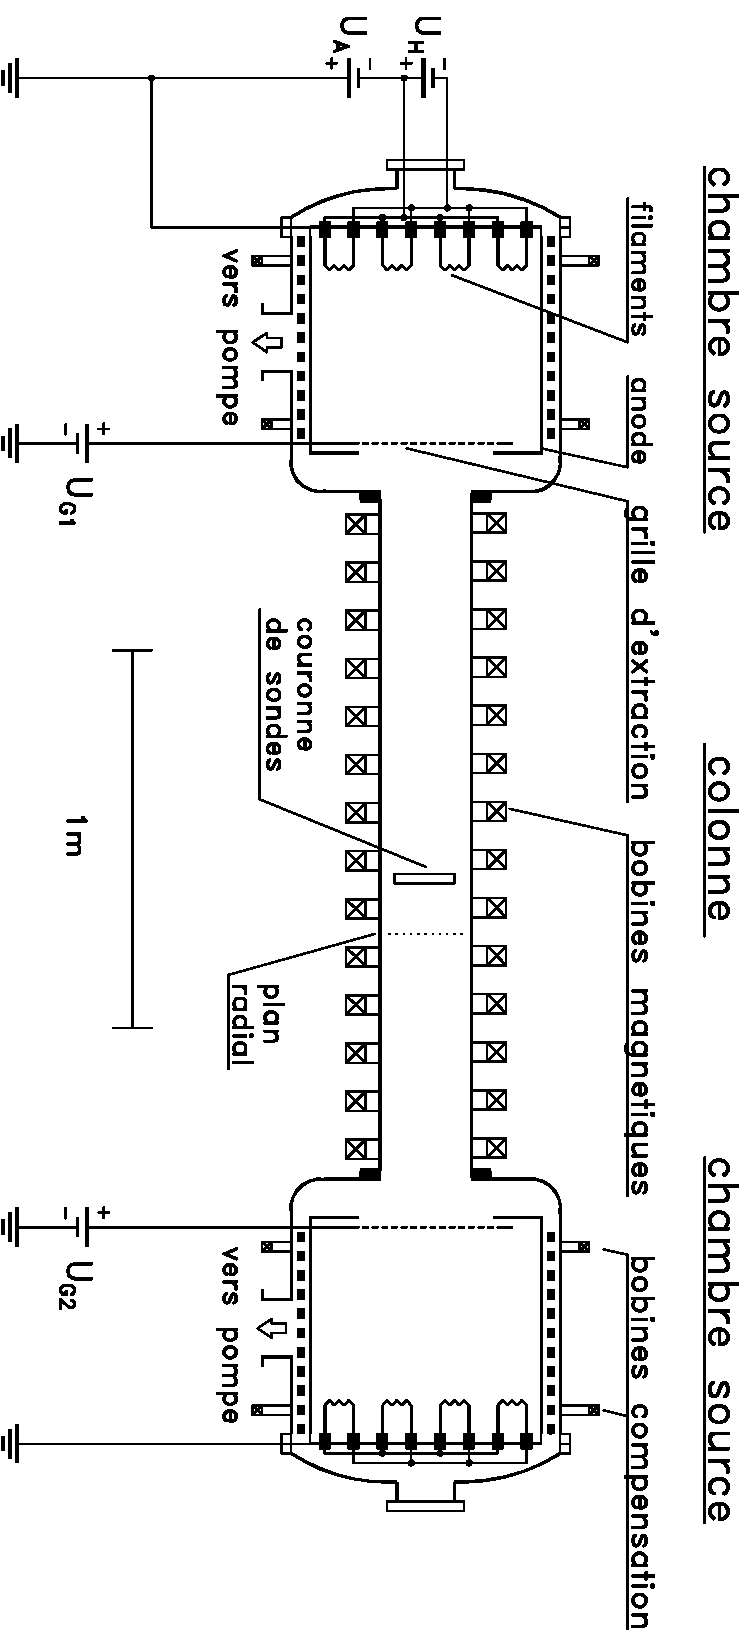
\epsfig{file={../fig/amkiwi2},width=12cm,angle=90}}

%bbllx=2.5cm,bblly=19.5cm,bburx=18.5cm,bbury=27.5cm}    
 \caption{Sch\'ema de la machine KIWI. Le plasma est produit dans la
chambre de gauche. Les ondes de d\'erive sont observ\'ees dans la partie
centrale.}
 \label{kiwi}
\end{figure}
%

La premi\`ere partie est constitu\'ee par la chambre de production
du plasma. La deuxi\`eme partie est la colonne \`a plasma dans laquelle
sont effectu\'es les diagnostics. La troisi\`eme est aussi une 
chambre \`a plasma mais elle n'est pas activ\'ee dans la s\'erie
d'exp\'eriences pr\'esent\'ee dans ce travail.

\subsection{La chambre de production}
%%%%%%%%%%%%%%%%%%%%
La chambre de production du plasma est une enceinte m\'etallique dans
laquelle a \'et\'e fait un vide pouss\'e (pression inf\'erieure \`a $10^{-6}\ {\rm
mbar}$). Une injection d'argon gazeux est faite par une pompe
situ\'ee dans la partie inf\'erieure de la chambre. La pression en argon
est $p_n=10^{-3}\ {\rm mbar}$. Au fond de la chambre se trouve un
arrangement de filaments de tungst\`ene qui, fortement chauff\'es 
par un courant intense qui les parcourt,
vont \'emettre des \'electrons par
\'emission 
thermoionique\index{thermoionique (\'emission)}
\cite{Kittel67,Ashcroft76}. 
Ces filaments sont polaris\'es n\'egativement par rapport \`a une anode
entourant la chambre et reli\'ee \`a la masse. Ainsi ces \'electrons
acqui\`erent une \'energie sup\'erieure \`a $15,7$ eV qui est l'\'energie
d'ionisation\index{ionisation} de l'atome d'argon. Des collisions\index{collision} entre ces \'electrons
\'energ\'etiques et les atomes neutres d'argon vont produire des ions
argon $Ar^+$. L'\'electron \'emis au cours de la collision est appel\'e
\'electron secondaire.

Pour augmenter la probabilit\'e de collision des \'electrons avec les
ato\-mes neu\-tres, l'anode reli\'ee \`a la masse a \'et\'e
recouverte de petits 
aimants  dispos\'es de mani\`ere \`a cr\'eer un champ magn\'etique
multipolaire. Chaque dip\^ole  cr\'ee localement un miroir
magn\'etique\index{miroir magn\'etique} \cite{Limpaecher73} assurant la
r\'eflection des \'electrons.  

Par un ph\'enom\`ene de gaine\index{gaine} (ph\'enom\`ene
\cite{Chen84} sur lequel nous 
allons revenir  
au moment de l'\'etude des sondes de Langmuir, annexe
\ref{chapdescplasma})  le potentiel 
\'electrique \`a 
l'int\'erieur de la chambre de production va s'\'etablir \`a une valeur
l\'eg\`erement positive et uniforme dans la chambre, \`a l'exception
des bords o\`u la variation du potentiel est tr\`es rapide, de
mani\`ere \`a 
satisfaire les conditions aux bords (potentiel nul sur l'anode,
potentiel fortement n\'egatif sur la cathode). C'est cette zone de grande
variation qui est appel\'ee
 gaine.


\subsection{La colonne \`a plasma}
%%%%%%%%%%%%%%%%%%%%
Dans la partie centrale de la machine se trouve une colonne m\'etallique
dans laquelle sont \'etudi\'ees les ondes de d\'erive\index{onde de
d\'erive}.  Elle mesure 1,80
m de long. Dans cette colonne
r\`egne un champ magn\'etique uniforme en premi\`ere approximation
(\`a 5 \% pr\`es) 
qui est n\'ecessaire \`a l'observation des ondes de d\'erive. Ce champ
magn\'etique est cr\'e\'e par des bobines conductrices qui entourent la
colonne et dans lesquelles circule un courant intense. Le champ
magn\'etique $B$ est alors proportionnel \`a l'intensit\'e $I$ du
courant dans les 
bobines, la relation de proportionnalit\'e \'etant : $B=2.23 I$, o\`u $B$
est exprim\'e en Gauss et $I$ en Amp\`ere.

Le passage du plasma de la chambre de production \`a la colonne
centrale est complexe. Il se fait par diffusion et 
gr\^ace \`a une grille d'extraction d'une transparence d'environ $50\ \%$.
Cette grille polaris\'ee positivement par rapport \`a $V_{g_1}$ attire les
\'electrons de la chambre
de production et repousse les ions. Un ph\'enom\`ene de gaine\index{gaine}
appara\^\i t donc aussi pr\`es de la grille d'extraction, o\`u la
variation de potentiel est tr\`es rapide.
Afin d'\'eviter que les lignes de champ $B$ cr\'e\'ees par les bobines
autour 
de la colonne ne rentrent dans la chambre de production, ce qui aurait
pour cons\'equence de canaliser les \'electrons \'emis par les filaments
directement dans la colonne (ph\'enom\`ene d'image magn\'etique), des
bobines dites de compensation \cite{Pierre86} ont \'et\'e plac\'ees au
niveau de la 
s\'eparation entre la chambre et la colonne. Elles ont pour but d'isoler
magn\'etiquement ces  deux r\'egions.


%
%\begin{figure}[htb]
% \centerline{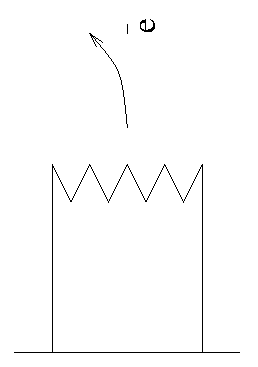
\epsfig{file={../fig/filament},width=4 cm,angle=0}}   
% \caption{Un filament parcouru par un courant intense \'emet des
%\'electrons.} 
% \label{filament}
%\end{figure}
%
%
\begin{figure}[htb]
 \centerline{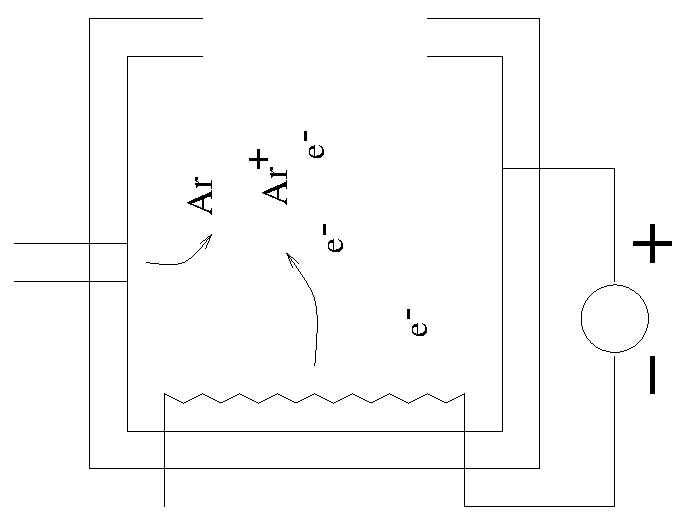
\epsfig{file={../fig/chambre},width=6 cm,angle=0}}   
 \caption{Sch\'ema de la chambre de production. Dans l'enceinte les
collisions entre les \'electrons de haute \'energie et les atomes
d'argon produisent le plasma.}
 \label{chambre}
\end{figure}
%


\begin{figure}[htb]
 \centerline{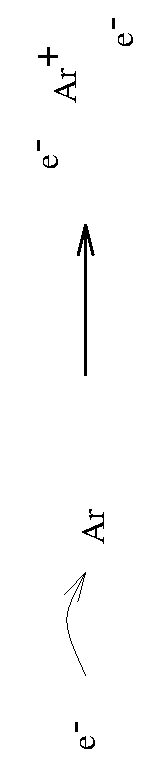
\epsfig{file={../fig/collision},width=8 cm,angle=0}}   
 \caption{Bilan de la r\'eaction de collision entre un atome neutre
d'argon et un \'electron. L'\'energie de l'\'electron incident doit
\^etre sup\'erieure \`a l'\'energie d'ionisation de l'argon.}
 \label{collision}
\end{figure}

%
%\begin{figure}[htb]
% \centerline{\epsfig{file={../fig/bouncing},width=6 cm,angle=0}}   
% \caption{Confinement \'electrostatique.}
% \label{confinement}
%\end{figure}
%


\begin{figure}[htb]
 \centerline{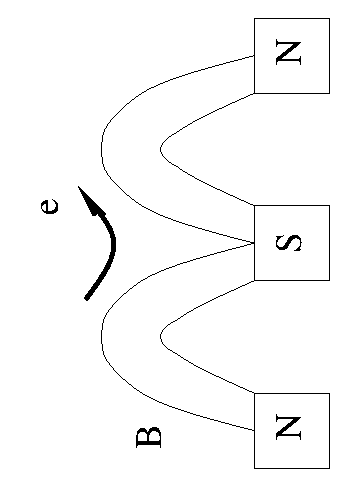
\epsfig{file={../fig/magmirror},width=6 cm,angle=0}}   
 \caption{Miroir magn\'etique. Les aimants plac\'es sur les parois de
la chambre de production augmentent la probabilit\'e de collision d'un
\'electron avec un atome neutre.}
 \label{miroir}
\end{figure}
%


%
\begin{figure}[htb]
 \centerline{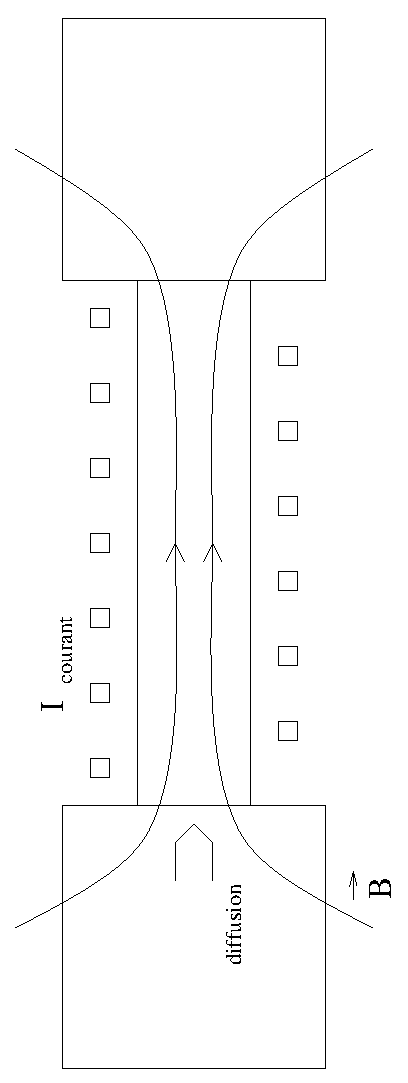
\epsfig{file={../fig/colon},width=\textwidth,angle=0}}   
 \caption{La colonne \`a plasma. Il y r\`egne un champ magn\'etique
uniforme en premi\`ere approximation.}
 \label{colonne}
\end{figure}
%


\begin{figure}
\begin{tabular}[t]{c}
\centerline{\subfigureA{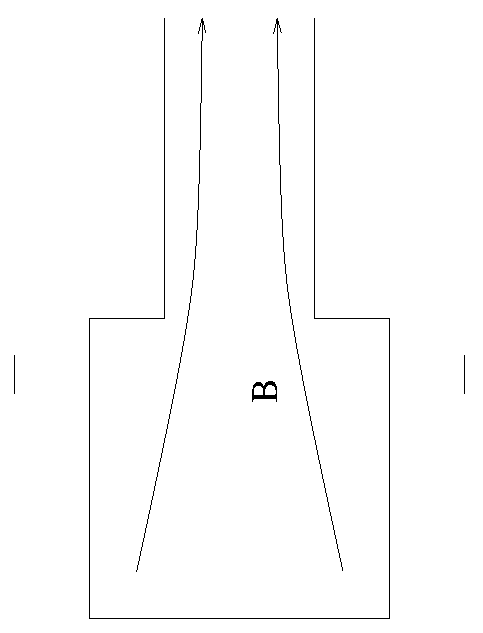
\epsfig{file={../fig/magmap},width=5cm,angle=0}} \hspace{1cm}
\subfigureA{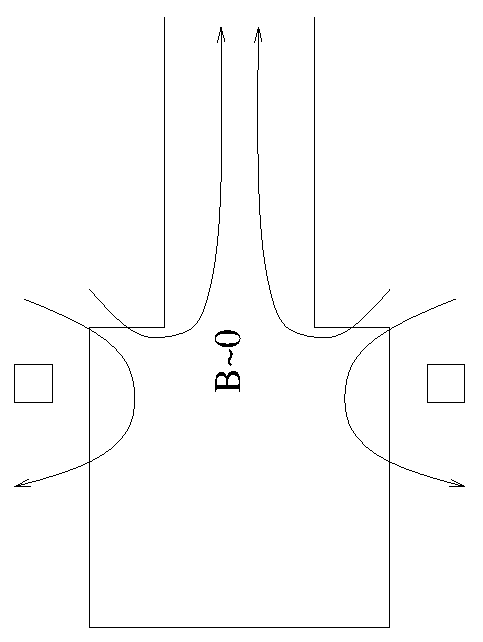
\epsfig{file={../fig/compcoil},width=5 cm,angle=0}}}
\end{tabular}                          
\caption{Champ $B$ sans et avec les bobines de compensation. Les
bobines de compensation isolent magn\'etiquement la chambre de la
colonne.}
\label{poitot}   
\end{figure}




\section{Les param\`etres de contr\^ole de l'exp\'erience}
%%%%%%%%%%%%%%%%%%%%
Nous donnons ici la liste des param\`etres de contr\^ole\index{param\`etre de contr\^ole} de
l'exp\'erience :

\begin{itemize}
\item     champ magn\'etique $B=70\ {\rm mT}$.
\item      pression de gaz neutre (argon)  $p_n=5.6\cdot 10^{-2} \ {\rm Pa}$.
\item      tension de d\'echarge            $U_{\rm d}=60\ {\rm V}$.
\item      courant de d\'echarge           $I_{\rm d}=13\ {\rm A}$.
\item      rayon du plasma (FWHM)          $R=0.1\ {\rm m}$.
\item      longueur de plasma               $L=1.8\ {\rm m}$.
\item tension de la grille 2 : $V_{g_2}=0$.
\item tension de la grille  : $V_{g_1}$, comprise entre $5.8$ et
$9.8\ {\rm V}$.
\end{itemize}






\section{Diagnostics sur l'\'etat d'\'equilibre}\label{sectionetat}
%%%%%%%%%%%%%%%%%%%%
En se donnant toutes les valeurs des param\`etres de contr\^ole, on
pourrait 
th\'eoriquement arriver \`a une description compl\`ete du syst\`eme. La
description que nous choisissons d'adopter est une description
fluide\index{fluide (description)} 
(voir la section \ref{sectiontheoriefluide}).
L'\'etat du syst\`eme est alors d\'ecrit par des fonctions de l'espace
et du temps qui sont :
\begin{itemize}
\item la densit\'e \'electronique $n_e$.
\item  la densit\'e ionique $n_i$. Dans l'approximation de
quasi-neutralit\'e (voir section \ref{sectiondebye}) on a $n_i\simeq n_e$.
\item le potentiel \'electrique $\phi$.
\item la temp\'erature \'electronique $T_e$.
\item  la temp\'erature ionique  $T_i$.
\item la vitesse \'electronique $v_e$.
\item la vitesse  ionique  $v_i$.
\end{itemize}

On suppose que le champ $B$ qui r\`egne dans le plasma est
constant, uniforme et ind\'ependant du temps.
Les fonctions densit\'e et potentiel
peuvent
\^etre d\'ecompos\'ees de la mani\`ere suivante :

\begin{equation}
n(r,z,\theta,t)=n^0(r,z)+\tilde{n}(r,z,\theta,t)
\end{equation}

\begin{equation}
\phi(r,z,\theta,t)=\phi^0(r,z)+\tilde{\phi}(r,z,\theta,t).
\end{equation}

Les fonctions index\'ees par $0$ d\'ecrivent l'\'etat d'\'equilibre,
$\tilde{n}$ et $\tilde{\phi}$ sont les perturbations\index{perturbation}. Ce sont ces
perturbations qui ont la forme d'ondes. Le sens qu'il faut donner au
mot ``onde'' sera pr\'ecis\'e au chapitre \ref{chapanalyse}.

La d\'eduction d'un mod\`ele pour la dynamique des perturbations \`a
partir des \'equations d'un mod\`ele \`a deux fluides
n\'ecessite 
la connaissance de l'\'etat d'\'equilibre (voir annexe
\ref{chapequationsflu}). La description de l'\'etat
d'\'equilibre \`a partir des \'equations de la physique est en
g\'en\'eral
difficile car elle correspond \`a la r\'esolution d'\'equations aux
d\'eriv\'ees 
partielles qui n\'ecessitent la connaissance pr\'ecise des
ph\'enom\`enes de 
bord entre autres choses.


Nous avons donc tent\'e une description de l'\'etat d'\'equilibre par des
mesures.
Voici quelques ordres de grandeur des caract\'eristiques du plasma :

\begin{itemize}
\item densit\'e \'electronique (au centre de la colonne)   $n_{\rm
e}=5\ 10^{16}\ {\rm m}^{-3}$.
\item temp\'erature \'electronique (au centre de la colonne)  $T_{\rm
e}=1,5\ {\rm eV}$.
\item temp\'erature ionique (au centre de la colonne)     $T_{\rm
i}=0,03\ {\rm eV}$.
\item densit\'e d'atomes  neutres $n_n=10^{19}\ {\rm m}^{-3}$. Cette
valeur est 
obtenue en utilisant l'\'equation d'\'etat $p_n=n_nk_BT_n$ en supposant
que les atomes neutres sont \`a la temp\'erature ambiante $T_n=300\
{\rm K}$.
\item degr\'e d'ionisation : $\alpha=n_n/n_e=5\ 10^{-3}$.
\end{itemize}

En fait la description compl\`ete de l'\'etat d'\'equilibre passe par la
donn\'ee des fonctions d'\'etat pour tout point de l'espace.
Nous pr\'esentons ici le r\'esultat de mesures radiales et axiales sur les
diff\'erentes grandeurs du plasma. Les mesures radiales ont \'et\'ees
faites sur une ligne situ\'ee axialement au quart de
la longueur de la colonne, en partant de la grille active.
Les mesures axiales ont \'et\'es faites sur l'axe de la colonne
($r=0$).

La figure Fig.\ref{nr} repr\'esente la densit\'e\index{densit\'e (\'electronique)}
\'electronique en 
fonction 
de $r$ et est mesur\'ee par deux m\'ethodes diff\'erentes. La premi\`ere
m\'ethode 
utilise le courant de saturation\index{courant de saturation} ionique $I_{i,sat}$ d'une sonde de
Langmuir\index{Langmuir (sonde de)}
(c'est-\`a-dire le courant qu'elle re\c coit lorsqu'elle est polaris\'ee
n\'egativement). La deuxi\`eme utilise le courant de saturation
\'electronique $I_{e,sat}$ (la sonde est polaris\'ee positivement). La
densit\'e 
\'electronique r\'eelle doit se trouver entre les deux mesures. La
densit\'e 
a typiquement un profil gaussien. La densit\'e d\'ecro\^\i t lorsque la
tension de grille $V_{g_1}$ augmente.
Pour le fonctionnement des sondes de Langmuir, voir
\cite{Hershkowitz93,Laframboise76,Rubinstein82,Rubinstein83} et
l'annexe \ref{chapdescplasma}.

\begin{figure}
{\centering
\begin{tabular}[t]{c}
\centerline{\subfigureA{\epsfig{file={../fig/prof1nr},width=7truecm,height=4truecm}}}\\
\centerline{\subfigureA{\epsfig{file={../fig/prof2nr},width=7truecm,height=4truecm}}}\\
\centerline{\subfigureA{\epsfig{file={../fig/prof4nr},width=7truecm,height=4truecm}}}\\
\centerline{\subfigureA{\epsfig{file={../fig/prof3nr},width=7truecm,height=4truecm}}}\\
\end{tabular} 
}
\caption{Densit\'e \'electronique (en $10^{10}\ {\rm cm}^{-3}$) en
fonction de $r$ (en mm). Trait
continu : \`a partir de $I_{e,sat}$,  trait pointill\'e : \`a partir de
$I_{i,sat}$. La valeur de la tension de grille $V_{g_1}$ est
rappel\'ee au dessus de chaque figure.}
\label{nr}
\end{figure}


La figure Fig.\ref{phir} repr\'esente le potentiel\index{potentiel} \'electrique en
fonction de $r$. Deux m\'ethodes ont l\`a aussi \'et\'e utilis\'ees.
La courbe en 
trait continu correspond \`a une \'evaluation de $\phi$ par  l'analyse
de la caract\'eristique courant--tension d'une sonde de Langmuir
plac\'ee en 
$r$. Cette technique \cite{Hansen94} est fiable mais la densit\'e
\'electronique doit \^etre 
forte (elle est donc inutilisable sur les bords du plasma). Par ailleurs
elle exige plusieurs mesures pour obtenir la courbe caract\'eristique
courant--tension. La courbe en trait continu a \'et\'e obtenue par une
sonde \'emissive \`a potentiel flottant. Cette technique est plus rapide
et elle est utilisable m\^eme pour des faibles densit\'es \'electroniques.
Mais elle 
est moins fiable. L'accord entre les deux types de mesure est bon. La
l\'eg\`ere dissym\'etrie des courbes correspond aux perturbations
provoqu\'ees  par la sonde.

On note un potentiel pr\`es de z\'ero volt au centre de la colonne
($r=0$). 
En s'\'eloignant de l'axe de la colonne le potentiel augmente jusqu'\`a
une valeur proche de la valeur du potentiel de la grille $1$.
Mais si $r$ augmente encore le potentiel doit d\'ecro\^\i tre \`a
nouveau  pour 
satisfaire la condition au bord du potentiel nul sur la paroi
m\'etallique de la
colonne. Toutefois, la mesure du potentiel \'electrique est rendue
impossible car la densit\'e du plasma dans cette zone est tr\`es faible. 

\begin{figure}
{\centering
\begin{tabular}[t]{c}
\centerline{\subfigureA{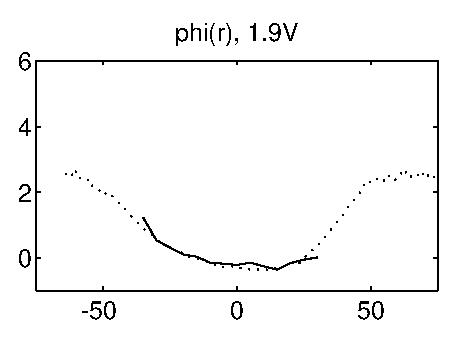
\epsfig{file={../fig/prof1phir},width=7truecm,height=4truecm}}}\\
\centerline{\subfigureA{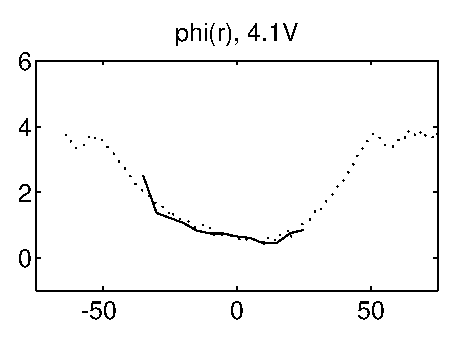
\epsfig{file={../fig/prof2phir},width=7truecm,height=4truecm}}}\\
\centerline{\subfigureA{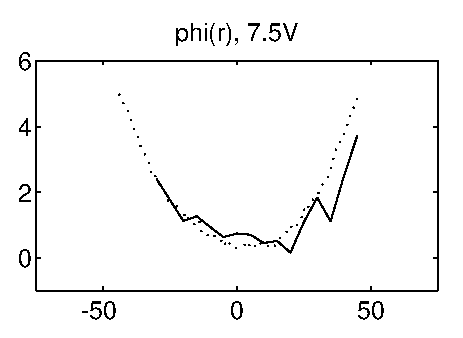
\epsfig{file={../fig/prof4phir},width=7truecm,height=4truecm}}}\\
\centerline{\subfigureA{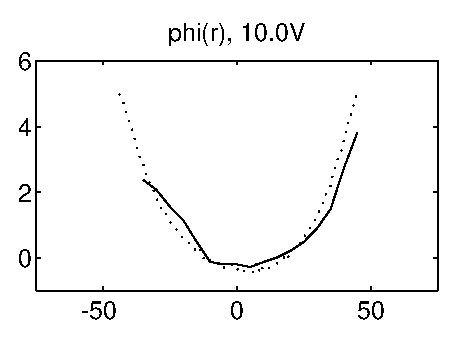
\epsfig{file={../fig/prof3phir},width=7truecm,height=4truecm}}}\\
\end{tabular} 
}
\caption{Potentiel \'electrique (en $V$) en fonction de $r$ (en mm).
La valeur de la tension de grille $V_{g_1}$ est 
rappel\'ee au-dessus de chaque figure. } 
\label{phir}
\end{figure}


La figure Fig.\ref{Ter} repr\'esente la temp\'erature\index{temp\'erature} \'electronique
en fonction de $r$,
mesur\'ee 
par des sondes de Langmuir. La temp\'erature est pratiquement
ind\'ependante de la tension de grille $V_{g_1}$.


\begin{figure}
{\centering
\begin{tabular}[t]{c}
\centerline{\subfigureA{\epsfig{file={../fig/prof1Ter},width=7truecm,height=4truecm}}}\\
\centerline{\subfigureA{\epsfig{file={../fig/prof2Ter},width=7truecm,height=4truecm}}}\\
\centerline{\subfigureA{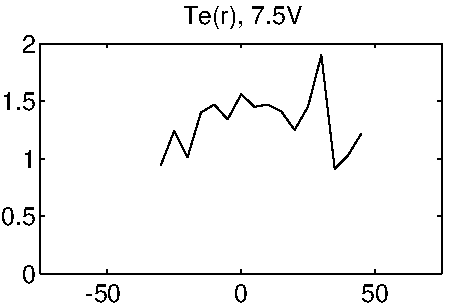
\epsfig{file={../fig/prof4Ter},width=7truecm,height=4truecm}}}\\
\centerline{\subfigureA{\epsfig{file={../fig/prof3Ter},width=7truecm,height=4truecm}}}\\
\end{tabular} 
}
\caption{Temp\'erature \'electronique  (en $eV$) en fonction de $r$. La valeur de la tension de grille $V_{g_1}$ est
rappel\'ee au-dessus de chaque figure.}
\label{Ter}
\end{figure}

La figure Fig.\ref{nz} repr\'esente la densit\'e \'electronique en
fonction 
de $z$. On note un gradient de densit\'e en fonction de $z$ qui
augmente avec la tension de grille. Par contre le rapport
$\frac{\nabla n^0}{n^0}$ est quasiment constant. 

Dans les figures Fig.\ref{nz}  \`a Fig.\ref{Tez}, l'origine des $z$
(coordonn\'ees cylindriques) a
\'et\'e prise \`a quelques millim\`etres \`a droite de la grille 1.
L'effet de gaine\index{gaine} 
ne s'observe donc pas sur ces mesures. La valeur $z=850$ mm correspond
\`a un point situ\'e \`a quelques centim\`etres \`a gauche du milieu
de la colonne. Rappelons que la colonne mesure 1,80 m\`etre de long.

La figure Fig.\ref{phiz}  repr\'esente  le potentiel
\'electrique en fonction de $z$. Le gradient en $z$ du potentiel
\'electrique est 
pratiquement constant dans la zone de mesure. Nous pr\'esentons dans
figure Fig.\ref{extrapotentiel} le potentiel \'electrique, tel qu'il
doit \^etre dans les diff\'erentes parties de la machine. Pour la
tracer, nous avons tenu compte des conditions aux bords et des
ph\'enom\`enes de gaine (voir section \ref{sectiondebye}). La mesure
d'une telle courbe pose d'\'evidents probl\`emes pratiques.

La figure Fig.\ref{Tez} repr\'esente   la temp\'erature \'electronique
en fonction de $z$. 
Le gradient de la temp\'erature en $z$ est voisin de z\'ero et la
temp\'erature $T_e$ est en premi\`ere approximation ind\'ependante de
la tension de grille $V_{g_1}$.

\begin{figure}
{\centering
\begin{tabular}[t]{c}
\centerline{\subfigureA{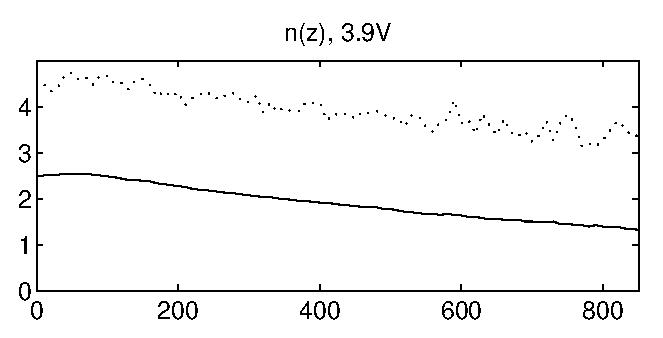
\epsfig{file={../fig/prof1nz},width=10truecm,height=4truecm}}}\\
\centerline{\subfigureA{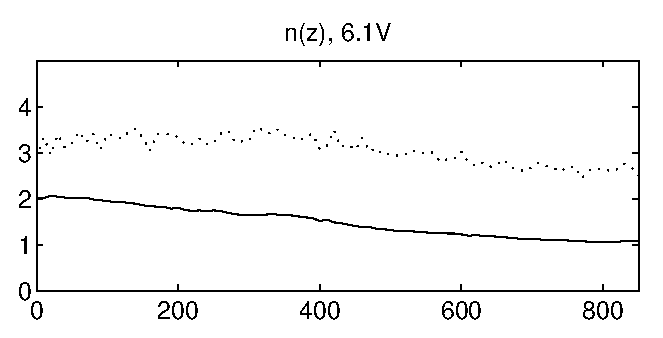
\epsfig{file={../fig/prof2nz},width=10truecm,height=4truecm}}}\\
\centerline{\subfigureA{\epsfig{file={../fig/prof3nz},width=10truecm,height=4truecm}}}\\
\end{tabular} 
}
\caption{Densit\'e \'electronique (en $10^{10} \ {\rm cm}^{-3}$) en
fonction 
de $z$ (en mm). Trait
continu : \`a partir de $I_{e,sat}$,  trait pointill\'e : \`a partir de
$I_{i,sat}$. La valeur de la tension de grille $V_{g_1}$ est
rappel\'ee au-dessus de chaque figure.}
\label{nz}
\end{figure}




\begin{figure}
{\centering
\begin{tabular}[t]{c}
\centerline{\subfigureA{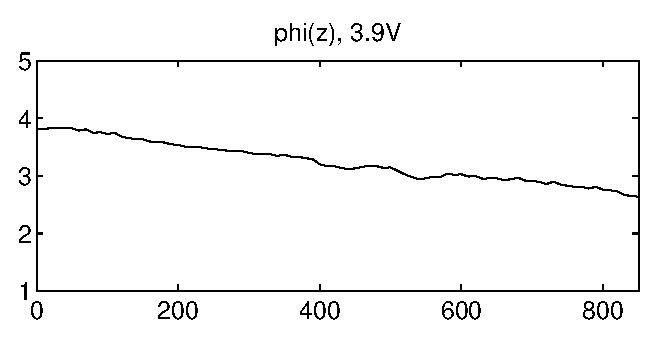
\epsfig{file={../fig/prof1phiz},width=10truecm,height=4truecm}}}\\
\centerline{\subfigureA{\epsfig{file={../fig/prof2phiz},width=10truecm,height=4truecm}}}\\
\centerline{\subfigureA{\epsfig{file={../fig/prof3phiz},width=10truecm,height=4truecm}}}\\
\end{tabular} 
}
\caption{Potentiel \'electrique  (en $V$) en fonction de $z$ (en mm).
La valeur de la tension de grille $V_{g_1}$ est 
rappel\'ee au-dessus de chaque figure.}
\label{phiz}
\end{figure}



\begin{figure}
{\centering
\begin{tabular}[t]{c}
\centerline{\subfigureA{\epsfig{file={../fig/prof1Tez},width=10truecm,height=4truecm}}}\\
\centerline{\subfigureA{\epsfig{file={../fig/prof2Tez},width=10truecm,height=4truecm}}}\\
\centerline{\subfigureA{\epsfig{file={../fig/prof3Tez},width=10truecm,height=4truecm}}}\\
\end{tabular} 
}
\caption{Temp\'erature \'electronique (en $eV$) en fonction de $z$ (en mm). La valeur de la tension de grille $V_{g_1}$ est
rappel\'ee au-dessus de chaque figure.}
\label{Tez}
\end{figure}



\begin{figure}[htb]
 \centerline{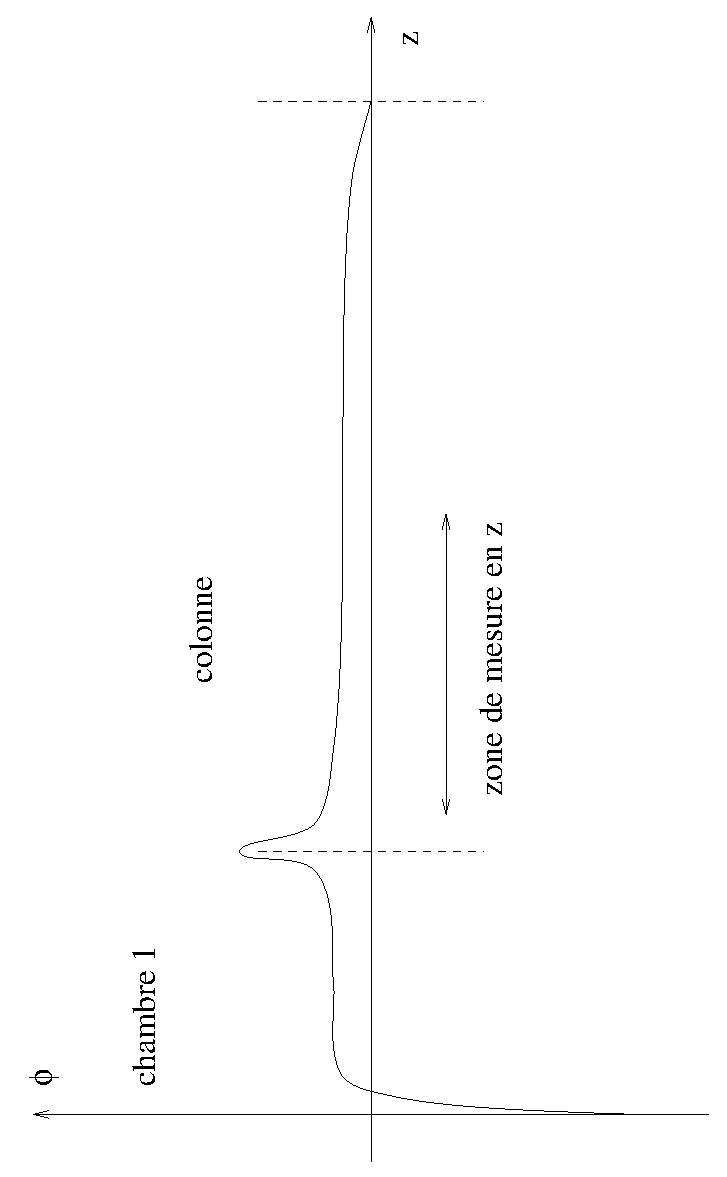
\epsfig{file={../fig/potentielz},width=\textwidth,angle=0}}
 \caption{Extrapolation du potentiel tel qu'il peut \^etre dans les
diff\'erentes parties de la machine (en fonction de $z$).}
 \label{extrapotentiel}
\end{figure}
%




L'obtention de ces diff\'erents profils par la th\'eorie n'est pas
ais\'ee. 
Aussi lorsque nous voudrons d\'eriver un syst\`eme d'\'equations pour la
dynamique des fluctuations \`a partir des \'equations fluides, nous
d\'efinirons les fluctuations par rapport \`a l'\'etat d'\'equilibre
mesur\'e exp\'erimentalement. 

\begin{rem}
Ces mesures sur l'\'etat d\'equilibre sont pr\'esent\'ees de mani\`ere
succintes. En effet, notre principal objet est l'\'etude de la
turbulence dans les fluctuations de densit\'e. N\'eanmoins, les
r\'esultats pr\'esent\'es ici nous seront utiles dans l'annexe
\ref{chapequationsflu}.
\end{rem}



\section{Diagnostics sur les perturbations}\label{sectiondiagpert}
%%%%%%%%%%%%%%%%%%%%
La grandeur choisie pour caract\'eriser les fluctuations\index{perturbation} est le signal
re\c cu par 64 sondes de Langmuir\index{Langmuir (sonde de)} dispos\'ees sur une couronne de $19$
cm de diam\`etre. Les pointes des sondes sont port\'ees par un cercle
de 
$7.5$ cm de diam\`etre (voir Fig.\ref{couronne}). Les sondes sont dans
le r\'egime de saturation 
\'electronique, et le signal re\c cu est donc, en premi\`ere
approximation, proportionnel aux
fluctuations de la densit\'e\index{densit\'e  (\'electronique)}  du plasma.



\begin{figure}
\centerline{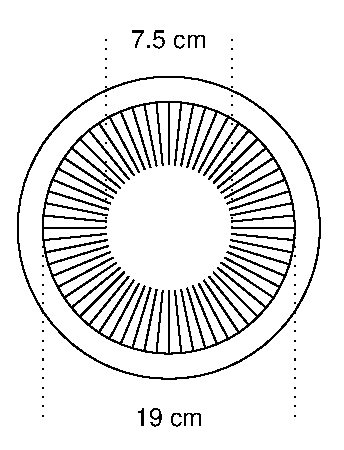
\epsfig{file={../fig/couronne},width=5truecm}}
\caption{La couronne de sondes de Langmuir. Elle est compos\'ee de 64
sondes et est plac\'ee au centre de la colonne \`a plasma.}
\label{couronne}
\end{figure}


La figure Fig.\ref{unesonde} repr\'esente le d\'etail d'une sonde.

\begin{figure}[htb]
 \centerline{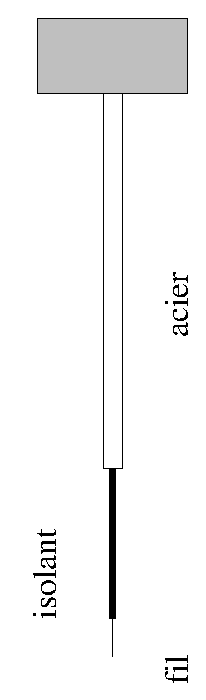
\epsfig{file={../fig/unesonde},width=60mm,angle=0}}
 \caption{D\'etail d'une sonde. L'extr\'emit\'e gauche est un fil de
tungst\`ene de 0,1 mm de diam\`etre et de 5 mm de long. L'isolant est
en c\'eramique.}
 \label{unesonde}
\end{figure}
%



Les signaux re\c cus  sont enregistr\'es
simultan\'ement sur les 64 sondes, pour 2048 pas de temps.
Le pas de temps est $\Delta t=10^{-6}\ \rm{s}$ pour toutes les figures
pr\'esent\'ees ici.

La tension de grille
$V_{g_1}$ est le seul param\`etre qui est modifi\'e dans la s\'erie de
mesures consid\'er\'ee. Ce param\`etre de contr\^ole\index{param\`etre de contr\^ole} (la tension
$V_{g_1}$) sera d\'esormais
d\'esign\'e par $\epsilon$. Nous pr\'esentons dans ce travail
l'analyse des perturbations $\tilde{n}_\epsilon$ pour dix valeurs de
$\epsilon$. Ces 10 valeurs $\epsilon_i$, ($i=1,\dots,10$) sont
donn\'ees dans la table 
Tab.\ref{values}. Les donn\'ees exp\'erimentales des fonctions
$\tilde n_{\epsilon(x,t)}$ seront d\'esign\'ees dans la suite $A_i$, o\`u
$i=1,\dots,10$.


\begin{table}[htb]
 \begin{center}
  \begin{tabular}{l|c|c|c|c|c|c|c|c|c|c}
d\'esignation  &${\epsilon}_1$& ${ \epsilon}_2$& ${\epsilon}_3$& ${ \epsilon}_4$& ${ \epsilon}_5$& ${ \epsilon}_6$& ${ \epsilon}_7$& ${ \epsilon}_8$& ${ \epsilon}_9$& ${ \epsilon}_{10}$\\
\hline
tension $V_{g_1}$(V) &5.8&5.9&6.1&6.5&7.1&7.6&7.8&8.0&8.4&9.8
  \end{tabular}
  \caption{Correspondance entre la d\'esignation $\epsilon_i$ et la
valeur de la tension de grille $V_{g_1}$.}
  \label{values}
\end{center}
\end{table}


La figure Fig.\ref{grayall} est une repr\'esentation en niveaux de
gris de 
l'\'evolution avec le param\`etre de contr\^ole de fonctions
$\tilde n_\epsilon(x,t)$ pour les dix valeurs de $\epsilon$
consid\'er\'ees 
dans la table Tab.\ref{values}. On voit que l'on passe d'un \'etat
pour lequel une structure spatio-temporelle de type onde est bien
identifiable vers un \'etat de turbulence\index{turbulence} faible pour lequel la
structure spatio-temporelle est plus complexe. Elle poss\`ede
n\'eanmoins une direction privil\'egi\'ee dans le plan $(x,t)$, o\`u
$x$ est l'angle azimathal. Dans
la section suivante nous proposons une premi\`ere analyse de ces
signaux, et au chapitre \ref{chapanalyse}, nous verrons comment
d\'ecomposer en structure spatio-temporelles les signaux pr\'esent\'es
dans la figure Fig.\ref{grayall}.

\begin{figure}
\begin{tabular}[t]{c}
\centerline{\subfigureA{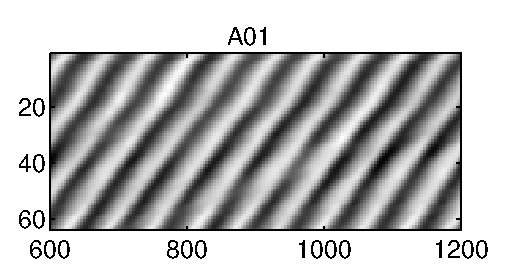
\epsfig{file={../fig/A01GraySig},width=6truecm,height=3truecm}}
\subfigureA{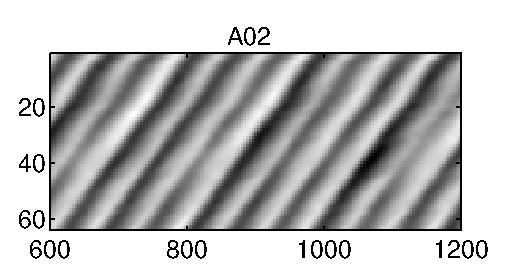
\epsfig{file={../fig/A02GraySig},width=6truecm,height=3truecm}}}\\
\centerline{\subfigureA{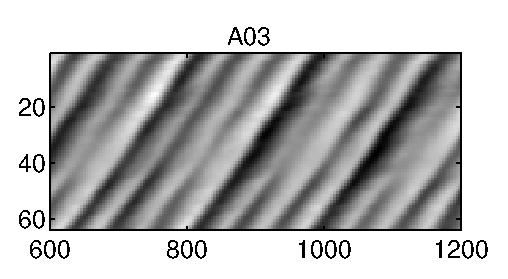
\epsfig{file={../fig/A03GraySig},width=6truecm,height=3truecm}}
\subfigureA{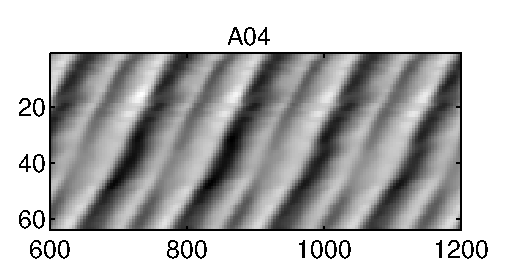
\epsfig{file={../fig/A04GraySig},width=6truecm,height=3truecm}}}\\
\centerline{\subfigureA{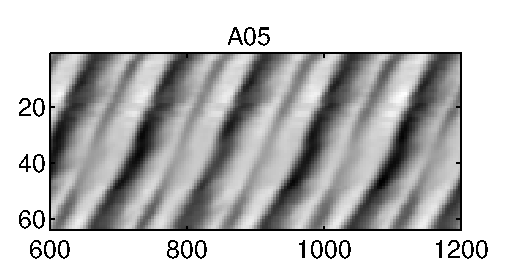
\epsfig{file={../fig/A05GraySig},width=6truecm,height=3truecm}}
\subfigureA{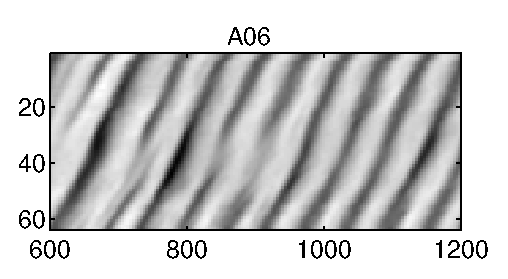
\epsfig{file={../fig/A06GraySig},width=6truecm,height=3truecm}}}\\
\centerline{\subfigureA{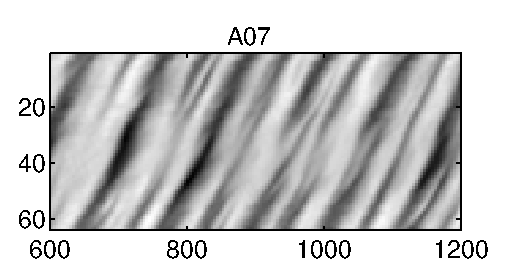
\epsfig{file={../fig/A07GraySig},width=6truecm,height=3truecm}}
\subfigureA{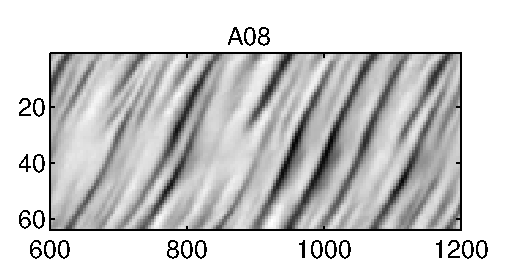
\epsfig{file={../fig/A08GraySig},width=6truecm,height=3truecm}}}\\
\centerline{\subfigureA{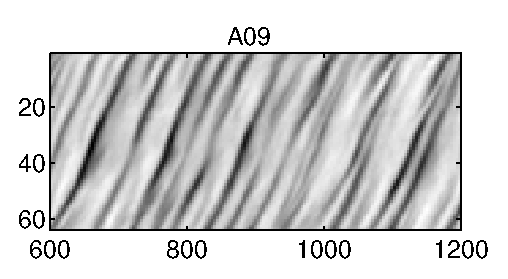
\epsfig{file={../fig/A09GraySig},width=6truecm,height=3truecm}}
\subfigureA{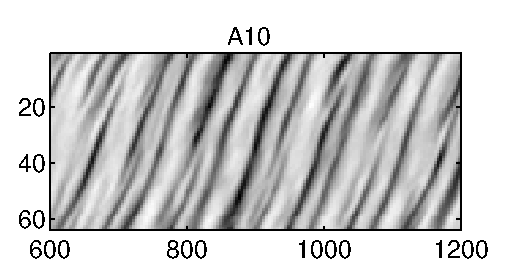
\epsfig{file={../fig/A10GraySig},width=6truecm,height=3truecm}}}
\end{tabular} 
\caption{Repr\'esentation en niveaux de
gris de 
l'\'evolution avec le param\`etre de contr\^ole de fonctions
$\tilde n_\epsilon(x,t)$ pour les dix valeurs de $\epsilon$
consid\'er\'ees.} 
\label{grayall}
\end{figure}





\section{Premi\`eres analyses}
%%%%%%%%%%%%%%%%%%%%%%%%%%%%%

Dans cette section, nous proposons une
\'etude rapide des donn\'ees (une \'etude plus approfondie sera faite
au chapitre \ref{chapanalyse}).
Dans la section pr\'ec\'edente nous avons repr\'esent\'e les fonctions
$\tilde n_\epsilon(x,t)$  en niveaux de gris. 
La figure Fig.\ref{probe} repr\'esente le signal re\c cu par la
premi\`ere sonde. La nature oscillante du signal nous invite \`a
appliquer \`a ce signal une transformation de Fourier. Les
transformations de Fourier sont pr\'esent\'ees dans la figure
Fig.\ref{fftprobe}. Ce type d'analyse, qui est purement temporel, nous
permet d\'ej\`a d'identifier des r\'egions de l'espace du param\`etre
$\epsilon$. Le signal ${A}_1$ correspond \`a une oscillation de
fr\'equence d'environ $15\ {\rm kHz}$. La pr\'esence des harmoniques de
cette fr\'equence montre que l'oscillation est l\'eg\`erement
non--lin\'eaire. 
Les signaux ${A}_2$ et ${A}_3$ correspondent \`a des \'etats
quasi--p\'eriodique\index{quasi-p\'eriodicit\'e} o\`u deux fr\'equences et leurs combinaisons
lin\'eaires sont pr\'esentes. Les signaux ${A}_4$ et ${A}_5$
sont relatifs \`a un accrochage de fr\'equence\index{accrochage de fr\'equence} . Les signaux suivants
poss\`edent un large spectre de Fourier. Nous avons affaire \`a une
turbulence\index{turbulence} faible.
\begin{figure}
\begin{tabular}[t]{c}
\centerline{\subfigureA{\epsfig{file={../fig/A01probe},width=120mm,height=17mm}}}\\
\centerline{\subfigureA{\epsfig{file={../fig/A02probe},width=120mm,height=17mm}}}\\
\centerline{\subfigureA{\epsfig{file={../fig/A03probe},width=120mm,height=17mm}}}\\
\centerline{\subfigureA{\epsfig{file={../fig/A04probe},width=120mm,height=17mm}}}\\
\centerline{\subfigureA{\epsfig{file={../fig/A05probe},width=120mm,height=17mm}}}\\
\centerline{\subfigureA{\epsfig{file={../fig/A06probe},width=120mm,height=17mm}}}\\
\centerline{\subfigureA{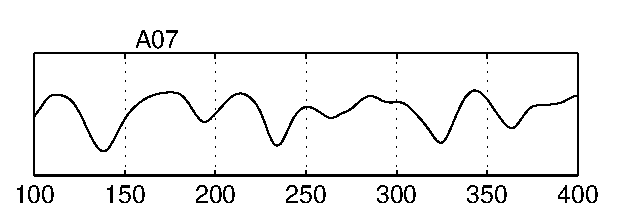
\epsfig{file={../fig/A07probe},width=120mm,height=17mm}}}\\
\centerline{\subfigureA{\epsfig{file={../fig/A08probe},width=120mm,height=17mm}}}\\
\centerline{\subfigureA{\epsfig{file={../fig/A09probe},width=120mm,height=17mm}}}\\
\centerline{\subfigureA{\epsfig{file={../fig/A10probe},width=120mm,height=17mm}}}\\
\end{tabular} 
\caption{Signal re\c cu par la sonde $1$ au cours du temps. En abscisse :
le temps en $10^{-6}\ {\rm s}$.} 
\label{probe}
\end{figure}



\begin{figure}
\begin{tabular}[t]{c}
\centerline{\subfigureA{\epsfig{file={../fig/A01fftprobe},width=60mm,height=35mm}}
\subfigureA{\epsfig{file={../fig/A02fftprobe},width=60mm,height=35mm}}}\\
\centerline{\subfigureA{\epsfig{file={../fig/A03fftprobe},width=60mm,height=35mm}}
\subfigureA{\epsfig{file={../fig/A04fftprobe},width=60mm,height=35mm}}}\\
\centerline{\subfigureA{\epsfig{file={../fig/A05fftprobe},width=60mm,height=35mm}}
\subfigureA{\epsfig{file={../fig/A06fftprobe},width=60mm,height=35mm}}}\\
\centerline{\subfigureA{\epsfig{file={../fig/A07fftprobe},width=60mm,height=35mm}}
\subfigureA{\epsfig{file={../fig/A08fftprobe},width=60mm,height=35mm}}}\\
\centerline{\subfigureA{\epsfig{file={../fig/A09fftprobe},width=60mm,height=35mm}}
\subfigureA{\epsfig{file={../fig/A10fftprobe},width=60mm,height=35mm}}}
\end{tabular} 
\caption{Transform\'ee de Fourier du signal
re\c cu par la premi\`ere sonde. Unit\'e de fr\'equence: $10^4\ {\rm
Hz}$.}  
\label{fftprobe}
\end{figure}


\chapter{Th\'eorie \`a l'ordre z\'ero des ondes de d\'erive}
%%%%%%%%%%%%%%%%%%%
Les ondes de d\'erive\index{onde de d\'erive} apparaissent dans les
plasmas non--homog\`enes magn\'etis\'es
\cite{Mikhailovsky83,Chen64,Chen65,Chen84,Hai70}, c'est-\`a-dire qui
pr\'esentent des gradients non-nuls dans les fonctions de la
description fluide (densit\'e, temp\'erature, champ
\'electrique, \dots). 
L'instabilit\'e\index{instabilit\'e} de l'onde de d\'erive est dite ``universelle''
parce qu'un syst\`eme physique est g\'en\'eriquement non--homog\`ene.
Les calculs pr\'esent\'es ici ne d\'ecrivent pas l'instabilit\'e
\cite{Mikhailovsky83,Ellis71,Ellis74,Ellis80} mais
seulement le r\^ole des diff\'erents gradients dans les pulsations des
ondes.

\section{Description particulaire}
%%%%%%%%%%%%%%%
Supposons que les particules\index{particulaire (description)} charg\'ees (ions et \'electrons)
entrent dans la colonne \`a plasma.
Dans cette colonne r\`egne un champ magn\'etique axial
(cr\'e\'e par les bobines) et un champ \'electrique axial cr\'e\'e
par la diff\'erence de potentiel $V_{g_1}-V_{g_2}$.
Le mouvement des particules est connu \cite{Chen84}.
Il d\'ecoule de la relation fondamentale de la dynamique :
\begin{equation}
m\frac{d v}{dt}=q v\wedge B+q E,
\end{equation}
si on n\'eglige la gravit\'e.
La trajectoire des particules se d\'ecompose 

\begin{itemize}
\item en une rotation
dans le plan $(x,y)$ \`a la pulsation cyclotron :

\begin{equation}
\omega_c=\frac{|q|B}{m}
\end{equation}

Si la particule rentre dans la colonne avec une vitesse
$v_{\perp}$, typiquement de l'ordre de la vitesse thermique
$v_{th}=\sqrt{\frac{2KT}{m}}$, alors le rayon de la trajectoire
est appell\'e rayon de Larmor\index{Larmor (rayon de)} :

\begin{equation}
r_L=\frac{v_{\perp}}{\omega_c}.
\end{equation}

\item en un mouvement rectiligne acc\'el\'er\'e du centre
guide\index{centre guide}
suivant l'axe $z$.
\end{itemize}

\begin{rem}
Dans cette configuration de champ $E$ et $B$, on n'observe pas 
de d\'erive du centre guide de la trajectoire. N\'eanmoins si le champ
$E$ n'\'etait pas parall\`ele au champ $B$, on observerait alors
une d\'erive du centre guide avec  une vitesse 
\begin{equation}
v_D=\frac{E\wedge B}{B^2}
\end{equation}
appel\'ee vitesse de d\'erive $E\wedge B$.
En fait il se trouve que la pr\'esence du plasma et les conditions aux
bords font que le champ \'electrique n'est pas celui qui r\`egne entre
deux plaques charg\'ees s\'epar\'ees par le vide. Nous renvoyons \`a
la section \ref{sectionetat} pour la description du potentiel
\'electrique dans la colonne.
\end{rem}


\section{Description fluide}
%%%%%%%%%%%%%%
\subsection{Mouvement d'ensemble du plasma}
%%%%%%%%%%%%%%%%%%%%%%%
Dans une description fluide\index{fluide (description)}, la vitesse
d'un \'el\'ement de fluide 
va \^etre diff\'erente de la vitesse des particules.
En effet, \'etudions le comportement d'un \'el\'ement de fluide
dans la m\^eme configuration de champ que pr\'ec\'edemment.
Supposons qu'il existe un gradient de densit\'e selon l'axe $x$.
Alors, comme le montre la figure Fig.\ref{diadrift} dans
laquelle nous avons repr\'esent\'e le mouvement de rotation
de chaque particule obtenu pr\'ec\'edemment, le bilan
du mouvement dans le plan $(x,y)$ r\'esulte en une d\'erive de
l'\'el\'ement de fluide\index{fluide (description)}. 
\begin{figure}[htb]
 \centerline{\epsfig{file={../fig/diadrift2},width=7 cm,angle=0}}   
 \caption{Un gradient de densit\'e peut cr\'eer une vitesse fluide
non--nulle dans un plasma, m\^eme si les particules ne se d\'eplacent
pas en moyenne. Le flux net de particules sur la surface de la bo\^\i te
est non nul. Il correspond \`a une vitesse fluide dirig\'ee vers le
bas.}
 \label{diadrift}
\end{figure}
%
Ce r\'esultat peut \^etre retrouv\'e \`a partir des \'equations fluides
des plasmas \cite{Braginskii65}.
Pour cela, \'ecrivons la 
conservation\index{conservation (\'equation de)} 
de la quantit\'e de mouvement
pour le fluide 
d'\'electrons, bilan dans lequel les collisions\index{collision} sont
n\'eglig\'ees 
\begin{equation}\label{me}
n^0_e m_e(\frac{\partial v^0_e}{\partial t}+({v}^0_e.\nabla
v^0_e))=en^0_e\nabla \phi^0 - e n_e v_e^0 \wedge B -\nabla p_e^0
\end{equation}
et pour le fluide d'ion :
\begin{equation}\label{mi}
n_i^0 m_i(\frac{\partial v^0_i}{\partial t}+({v}^0_i.\nabla v^0_i))=-en^0_i\nabla \phi^0 + en_i^0 v^0_i \wedge B -\nabla p^0_i.
\end{equation}
Nous cherchons des solutions stationnaires.
Supposons : 
\begin{itemize}
\item \`a l'ordre z\'ero, le champ $E$ est dirig\'e selon
l'axe $z$.
\item les gaz d'\'electrons et d'ions 
parfaits\index{gaz parfait (approximation de)} ($p^0_a=n_a^0k_BT^0_a$
o\`u $a=e,i$).
\item $T^0_i=0$.
\item l'inertie de \'electrons nulle ($n^0_e m_e(\frac{\partial v^0_e}{\partial t}+({v}^0_e.\nabla v^0_e))=0$)
\item $n^0=n^0_e=n^0_i$ pour cet \'etat.
\end{itemize}

L'\'equation de conservation\index{conservation (\'equation de)}  de la
quantit\'e de mouvement des \'electrons projet\'ee sur le plan
perpendiculaire \`a $B$ est :
\begin{equation}
0=en^0v_e^0\wedge B +k_B T_e^0\nabla n^0.
\end{equation}
D'o\`u en multipliant vectoriellement par $B$ :
\begin{equation}\label{eqformulevit}
v_{e,\perp}^0=-\frac{k_B T_e^0 \nabla_r n^0}{e B n^0} e_\theta,
\end{equation}
o\`u $e_\theta$ est le vecteur polaire de la base $(e_r,e_\theta,e_z)$.
Le mouvement global du fluide d'\'electrons
est un mouvement de rotation de la colonne autour de l'axe $z$ auquel
se superpose une acc\'el\'eration en $z$ (pour voir cette
acc\'el\'eration, il faut projeter  l'\'equation de conservation de la
quantit\'e de mouvement des \'electrons sur l'axe $z$).
La vitesse des ions est donn\'ee par une \'equation similaire \`a
l'\'equation \ref{eqformulevit}. En effet, l'inertie des ions peut
elle aussi \^etre n\'eglig\'ee, puisque l'on cherche des solutions
stationnaires, ind\'ependantes de $\theta$. Mais avec l'hypoth\`ese
$T_i^0=0$, le fluide d'ions ne tourne pas.

Nous verrons \`a l'annexe \ref{chapequationsflu} les modifications
qu'il faut apporter aux calculs de l'\'etat d'\'equilibre si l'on tient
compte du champ \'electrique perpendiculaire \`a $B$.

\subsection{Th\'eorie simple d'ondes de d\'erive}
%%%%%%%%%%%%%%%%%%%%%%%%%%%%%%%%
Nous cherchons\index{onde de d\'erive} maintenant \`a d\'ecrire
l'\'evolution de perturbations 
par rapport \`a l'\'etat \`a l'ordre z\'ero.
Supposons que :
\begin{itemize}
\item les vitesses s'\'ecrivent $v_a=\tilde{v}_a+v_a^0$
avec $v_i^0=0$ et $v_e^0=-\frac{k_B T_e \nabla_x n^0}{e B n^0} e_{\theta}$.
\item le champ $E_\perp$ s'\'ecrit : $E_\perp=0+\tilde{E}_\perp$.
\item les densit\'es s'\'ecrivent $n_a=n_0+\tilde{n}_a$. 
 il y a quasi-neutralit\'e\index{quasi-neutralit\'e} : $\tilde{n}_e=\tilde{n}_i=\tilde{n}$.
\item les gaz sont consid\'er\'es 
parfaits\index{gaz parfait (approximation de)}  : $p_a=n_ak_BT_a$.
\item $T_e$, $T_i$ ont pour valeurs celles de l'\'etat d'\'equilibre.
\end{itemize}
L'hypoth\`ese $E_\perp^0=0$ n'est pas v\'erifi\'ee dans notre cas. Le
calcul pr\'esent\'e \cite{Chen84,Mikhailovsky83} est destin\'e \`a introduire les ondes de d\'erives.
La conservation\index{conservation (\'equation de)} 
 de la quantit\'e de mouvement pour le fluide d'ions donne
au premier ordre :
\begin{equation}
m_i\tilde{n}\frac{d\tilde{v}_{i,\perp}}{dt} =
q\tilde{n}_{i,\perp}(\tilde{E}_{\perp}+\tilde{v}_{i,\perp}\wedge B). 
\end{equation}
Dans le cas o\`u l'on peut n\'egliger la d\'eriv\'ee particulaire
$\frac{d}{dt}$, la perturbation de la vitesse ionique perpendiculaire
est :
\begin{equation}
\tilde{v}_{i,\perp}=\frac{\tilde{E}_\perp\wedge B}{B^2}.
\end{equation}
L'\'equation de continuit\'e pour le fluide d'ions s'\'ecrit :
\begin{equation}\label{eqcontele}
\frac{\partial\tilde{n}/n^0}{\partial
t}+\tilde{v}_\perp\frac{\nabla_\perp{n^0}}{n^0}=0,
\end{equation}
en supposant que le terme $\tilde{v}_\perp\frac{\nabla_\perp{n_0}}{n^0}$
l'emporte sur les autres termes de la divergence.

\begin{rem}
Cette approximation est donn\'ee dans les livres introduisant les
ondes de d\'erive\index{onde de d\'erive}
\cite{Chen84,Mikhailovsky83}. Elle n'est pas 
justifi\'ee 
rigoureusement et une \'etude plus d\'etaill\'ee du type Hasegawa-Mima 
que nous rappelons \`a l'annexe \ref{chapequationsflu} montre qu'il
faut tenir 
compte d'autres termes.
\end{rem}

Une relation entre le potentiel\index{potentiel} 
\'electrique $\tilde{\phi}$ et
$\tilde{n}$ s'obtient par 
l'\'equation de la dynamique parall\`ele des \'electrons \cite{Chen84}. 
Les \'electrons ob\'eissent
\`a la relation de Boltzmann\index{Boltzmann (statistique de)}
\begin{equation}\label{eqbold}
\frac{\tilde{n}}{n_0}=\frac{e\tilde{\phi}}{k_B T_e}.
\end{equation}
L'\'equation d\'ecrivant la dynamique du potentiel \'electrique
$\tilde{\phi}$ est, en combinant les \'equations \ref{eqcontele} et
\ref{eqbold} 
\begin{equation}
\frac{\partial \tilde{\phi}}{\partial
t}=\frac{k_B T_e\nabla_\perp\tilde\phi\wedge B}{e
B^2}.\frac{\nabla_\perp n^0}{n^0}. 
\end{equation}
En supposant que le gradient de $n^0$ est dirig\'e suivant $e_r$, le
produit scalaire pr\'ec\'edent se simplifie, et l'on obtient :
\begin{equation}
\frac{\partial \tilde{\phi}}{\partial
t}=\frac{k_B T_e\partial_\theta\tilde\phi\wedge
B}{r e B^2}.\frac{\partial_r n^0}{n^0}.
\end{equation}
Par une transformation de Fourier en $\theta$, on obtient une relation
de dispersion :
\begin{equation}\label{equareladispli}
\frac{\omega}{m}=-\frac{k_B T_e\nabla_r n_0}{r e B n_0},
\end{equation}
o\`u $m$ est la variable conjugu\'ee de $\theta$ par transformation de
Fourier. 

Une telle th\'eorie simple implique que les signaux mesur\'es par
notre couronne de sonde de Langmuir doivent \^etre de la forme :
\begin{equation}\label{equsimplesuper}
\tilde n(x,t)=\sum \alpha_m \cos(m \theta-\omega t+f_m),
\end{equation}
o\`u les nombres $m$ et $\omega$ v\'erifient la relation de dispersion
donn\'ee par l'\'equation (\ref{equareladispli}). Il faut noter que
l'unicit\'e de la solution est assur\'ee par la prise en compte des
conditions aux limites et des conditions initiales. 
La figure Fig.\ref{nr} doit nous permettre d'atteindre la valeur de
$\frac{\nabla_r n_0}{n_0}$ correspondant \`a la position des sondes de
la couronne ($r=3,75\ {\rm cm}$), mais l'incertitude sur la mesure de
$n^0$ est particuli\`erement grande pour cette valeur de $r$. Une
fr\'equence de $1,7\ 10^{4}\ {\rm Hz}$ qui correspond \`a un mode
$m=3$ pour l'ensemble de donn\'ees $A_1$ (voir figure
Fig.\ref{grayall} et 
Fig.\ref{fftprobe}) implique par exemple une valeur de $0,4\ {\rm
m}^{-1}$ pour la quantit\'e $\frac{\nabla_r n_0}{n_0}$.

Dans la suite du document, nous allons \'etudier comment aller au-del\`a
de la th\'eorie lin\'eaire, en particulier voir comment un \'ecart \`a
une solution de la forme de l'\'equation (\ref{equsimplesuper}) permet
d'interpr\'eter des figures comme celle relative \`a $A_{10}$ dans la
figure Fig.\ref{grayall}.




\part[L'outil d'analyse : \hspace{25 truecm}\null { } la D\'ecomposition Bi--Orthogonale]{L'outil d'analyse : la D\'ecomposition Bi--Orthogonale}
%%%%%%%%%%%%%%%%%%%

\chapter{La D\'ecomposition Bi--Orthogonale, g\'en\'eralit\'es}
%%%%%%%%%%%%%%%%%%%%%%%%

\section{Introduction}
%%%%%%%%%%%%%%%%%%%

Le but de ce chapitre est d'introduire la d\'ecomposition
bi-orthogonale\index{bi-orthogonale (d\'ecomposition)}. La
d\'ecomposition bi-orthogonale (DBO) est une m\'ethode 
qui donne le plus petit espace fonctionnel dans 
lequel on peut observer
la dynamique associ\'ee \`a une fonction spatio-temporelle.

L'op\'eration math\'ematique, l'analyse spectrale d'un op\'erateur \`a
noyau, \`a laquelle correspond la DBO
est connue depuis bien longtemps
\cite{Courant24,VonNeuman35}. Les statisticiens l'ont utilis\'ee
\cite{Loeve55,Karhunen44}. Elle
est parfois appel\'ee d\'ecomposition de
Karhunen-Lo\`eve\index{Karhunen-Lo\`eve (d\'ecomposition de)}.
Le probl\`eme
spectral de la DBO est connu en analyse num\'erique sous le nom de
D\'ecomposition en Valeurs 
Singuli\`eres\index{valeurs singuli\`eres (d\'ecomposition en)}
\cite{Press92}. 
L'Analyse en Composantes Principales (ACP\index{ACP}) se formalise d'une
mani\`ere tr\`es voisine (voir la section \ref{sectionacp}).
La d\'ecomposition bi-orthogonale a \'et\'e introduite
 pour l'analyse de signaux turbulents
spatio-temporels \cite{Lumley72,Lumley81}. 
Depuis, cette m\'ethode a \'et\'e \'etudi\'ee th\'eoriquement
\cite{Guyonnet91,Aubry88,Aubry91a,Aubry91b,Aubry92,Aubry94,Aubry95a,Aubry95b}  
et appliqu\'ee \`a de nombreux probl\`emes exp\'erimentaux
\cite{Dudok94,Kolodner95,Vautard89,Vautard92}. 
Le lecteur pourra aussi consulter \cite{Lumley90,Sirovich89,Broomhead86,Newell88}

\section{Dynamique\index{dynamique} et structures
spatiales\index{structure spatiale}}
%%%%%%%%%%%%%%%
Soit une fonction de l'espace et du temps $u(x,t)$,
d\'efinie sur le pav\'e $X \times T$ \`a valeurs r\'eelles. Nous
consid\'erons aussi les espaces
$H(X)$, un espace de Hilbert d\'efini sur les fonctions du segment $X$,
et $H(T)$, un espace de Hilbert d\'efini sur les fonctions du
segment $T$. Les produits scalaires dont sont muni ces espaces peuvent
\^etre 
choisi selon le probl\`eme \'etudi\'e; dans notre cas, nous utiliserons
toujours les produits scalaires de $L^2(X)$ et $L^2(T)$.
La fonction $u$ est  le signal exp\'erimental que fournissent les
sondes au cours du temps;  $x$ sera la variable spatiale indexant la
position de chaque sonde.
\`A cette fonction $u(x,t)$ on peut associer :

\begin{itemize}
\item une famille de fonctions de $x$ d\'ependant du param\`etre $t$
d\'efinie par : 
\begin{equation}
\forall x \in X,\ \xi_t(x)=u(x,t).
\end{equation}
\item une famille de fonctions de $t$ d\'ependant du param\`etre $x$ :
\begin{equation}
\forall t \in T,\ \eta_x(t)=u(x,t).
\end{equation}
\end{itemize}

L'\'evolution du vecteur  $\xi_t$ au cours du temps constitue
la dynamique. Celle-ci est incluse dans l'espace $H(X)$ qui est
appel\'e espace des configurations\index{configurations (espace des)}.
L'ensemble des fonctions $\eta_x$ d\'efinit la structure spatiale.
La structure spatiale
est incluse dans l'espace $H(T)$ qui est appel\'e espace des s\'eries
temporelles\index{s\'eries temporelles (espace des)}.
La d\'ecomposition bi-orthogonale fournit le plus petit sous-espace
$\chi(X)$ de $H(X)$ qui contient toute la trajectoire
et le plus petit sous-espace $\chi(T)$ de $H(T)$ qui
contient toute la structure spatiale.

\section{Op\'erateur associ\'e au signal}
%%%%%%%%%%%%%%%%%%%
\`A tout signal spatio-temporel $u(x,t)$ on peut associer
un op\'erateur $U$ de $H(X)$ dans $H(T)$ qui est d\'efini par son
action sur les 
fonctions de $H(X)$ :
\begin{equation}\label{equdefU}
U\phi(x)=\int_X u(x,t)\phi(x)dx.
\end{equation}
L'adjoint de $U$ est $U^+$, de $H(T)$ dans $H(X)$, d\'efinit par :
\begin{equation}\label{equdefUa}
U^+\psi(t)=\int_Tu(x,t)\psi(t)dt.
\end{equation}


\begin{rem}
Pour que les \'equations (\ref{equdefU}) et (\ref{equdefUa})
d\'efinissent bien un op\'erateur lin\'eaire born\'e, il faut bien
s\^ur imposer certaines conditions \`a $u(x,t)$.
Dans le cas pratique de nos signaux exp\'erimentaux,
le segment $X$ est remplac\'e par l'ensemble des positions des
sondes $E_X=\{x_i\}_{i=1,...,P}$ o\`u $P$ est le nombre de sondes
et le segment $T$ est remplac\'e par l'ensemble des instants
auxquels se font les mesures $E_T=\{t_i\}_{i=1,...,Q}$ o\`u $Q$
est le nombre de saisies.
Le signal exp\'erimental est donc un tableau
$u(x_i,t_j)$.
La d\'efinition pr\'ec\'edente de l'op\'erateur $U$ devient alors
une d\'efinition matricielle :
\begin{equation}
(U\phi)_i=U_{i j}\phi_j
\end{equation}
et
\begin{equation}
(U^+\psi)_i=U^+_{i j}\psi_j,
\end{equation}
o\`u on a utilis\'e la convention de l'indice r\'ep\'et\'e.
L'op\'erateur $U$ est d\'efini par $U_{i j}=u(x_i,t_j)$.

\end{rem}

\section{D\'efinition de la DBO}
%%%%%%%%%%
\subsection{Analyse spectrale}
%%%%%%%%%%%%%%%%%%%%%%%%%%
Dans ce qui suit, nous nous pla\c cons dans le cas o\`u l'op\'erateur
$U$ d\'efini par l'\'equation (\ref{equdefU}) poss\`ede un spectre
discret. 
\begin{defn}\label{defbod1}
On dit que l'on a effectu\'e la d\'ecomposition bi-orthogonale
du signal $u(x,t)$ si on a \'ecrit $u(x,t)$ sous la forme :
\begin{equation}\label{dec}
u(x,t)=\sum_{k=1}^{N}\alpha_k\phi_k(x)\psi_k(t),
\end{equation}
avec $\alpha_1>\alpha_2>...>\alpha_N>0$ et si on a les conditions
d'orthogonalit\'e :
\begin{equation}
\langle \phi_k\mid \phi_l\rangle =\delta_{k,l}\ {\rm et}\ \langle \psi_k\mid \psi_l\rangle =\delta_{k,l},
\end{equation}
o\`u $\delta_{k,l}$ repr\'esente le symbole de Kronecker. $N$ peut
\^etre fini ou infini.
\end{defn}

Les fonctions de $x$ sont appel\'ees les {\bf topos\index{topo}}, les fonctions
de $t$ sont appel\'ees les {\bf chronos\index{chrono}}, les $\alpha_k$ sont
appel\'es les {\bf poids}\index{poids} ou {\bf valeurs propres}.
$N$ (fini ou infini) est appel\'e la dimension\index{dimension d'un signal} du signal.

\begin{rem}
Dans le cas d'une matrice, l'entier $N$ est appel\'e rang de la matrice
$U$. 
\end{rem}
Cette d\'efinition revient \`a \'ecrire l'op\'erateur $U$ comme
\begin{equation}
U=\sum_{k=1}^{N}\mid \psi_k\rangle \alpha_k\langle \phi_k\mid .
\end{equation}
Une d\'efinition, en principe plus g\'en\'erale, de la DBO est de 
pr\'esenter la recherche des topos et
chronos comme la recherche de la solution d'un probl\`eme spectral :

\begin{defn}\label{defbod2}
La d\'ecomposition bi-orthogonale d'un signal $u(x,t)$
est la solution $(\phi,\psi,\alpha)$
 du probl\`eme spectral suivant :
\begin{equation}
U\phi=\alpha\psi
\end{equation}
\begin{equation}
U^+\psi=\alpha\phi.
\end{equation}
\end{defn}

On voit que si le spectre $\alpha$ de $U$ est discret
alors cette d\'efinition implique l'existence d'une d\'ecomposition
de la forme donn\'ee par l'\'equation (\ref{dec}).
Le spectre de $U$ est discret en particulier si $U$ est compact.

\begin{rem}
On voit que la condition $\alpha_k>0$ de la d\'efinition
\ref{defbod1} peut toujours \^etre
faite puisque  le signe de $\alpha_k$ peut \^etre absorb\'e par une des
deux fonctions propres. 
\end{rem}

Pour les signaux exp\'erimentaux r\'eels, $U$ est une matrice $p\times q$
et le spectre est n\'ecessairement discret.
La dimension\index{dimension d'un signal} du signal est alors inf\'erieure ou \'egale au 
minimum des deux entiers $p$ et $q$.
Nous pouvons d\'emontrer le th\'eor\`eme suivant :
\begin{thm}
Soit $u(x,t)$ une fonction d\'efinie sur $X \times T$.
Soit $e_i$ une base de $\chi(X)=Ker\ U^\perp$. 
Soient $f_i$ les images normalis\'ees des $e_i$ par $U$.
Donc 

\begin{equation}
U=\sum a_i \mid f_i\rangle \langle e_i\mid .
\end{equation}
Alors, la d\'efinition \ref{defbod1} est \'equivalente \`a la
d\'efinition \ref{defbod2}.
\end{thm}
\begin{pf}
Il suffit d'ins\'erer la relation de fermeture 
\begin{equation}
\sum \mid e_i\rangle \langle e_i\mid =P
\end{equation}

et 
\begin{equation}
\sum \mid f_i\rangle \langle f_i\mid =\tilde P
\end{equation}
(o\`u $P$ est le projecteur sur
$\chi(X)$, le support \`a droite de $U$, et $\tilde P$, celui sur
$\chi(T)=Ker\ (U^*)^\perp$, le support \`a gauche de $U$) pour montrer
que la d\'efinition  \ref{defbod1} 
implique la d\'efinition \ref{defbod2}.
Inversement, la d\'efinition \ref{defbod2} implique la d\'efinition
\ref{defbod1}  en multipliant par les op\'erateurs $U^+$ et $U$ 
les \'equations spectrales.
\end{pf}

\section{G\'en\'eralisation \`a des fonctions de $\vec r\in R^3$ et de $t$} \label{secgeneplus}
%%%%%%%%%%%%%%%%%%%%%%%

La d\'efinition de la d\'ecomposition bi-orthogonale pour des fonctions
de $\vec r$ et $t$ o\`u 
$\vec r$ est un vecteur de $R^3$  est en principe la m\^eme que pour une
simple fonction de 
$x$ et $t$ sauf que le produit scalaire spatial doit \^etre compris au
sens de $L^2(R^3)$.
\begin{equation}
u(\vec r,t)=\sum_{k=1}^{N} \alpha_k \phi_k(\vec r)\psi_k(t),
\end{equation}
avec $\alpha_1\geq\alpha_2\geq\dots\alpha_N>0$ et 
$\langle \phi_k\mid \phi_{k^\prime}\rangle =\delta_{k,k^\prime}$ et
$\langle \psi_k\mid \psi_{k^\prime}\rangle =\delta_{k,k^\prime}$.

Le probl\`eme du lien entre la d\'ecomposition bi-orthogonale d'une
fonction $u(x,y,z,t)$ et la d\'ecomposition bi-orthogonale de la
fonction $u_{y_0,z_0}(x,t)$ est tr\`es important dans la pratique.
La question fondamentale :''Connaissant la DBO de  $u_{y_0,z_0}(x,t)$,
que peut--on dire de la DBO de $u(x,y,z,t)$ ?'', n'a pas encore de
r\'eponse g\'en\'erale. 
Toutefois, il existe un cas simple pour lequel on peut d\'eduire la
d\'ecomposition bi--orthogonale de $u_{y_0,z_0}(x,t)$ \`a partir de
celle de
$u(x,y,z,t)$. C'est le cas o\`u les topos $\phi_k$ de $u(x,y,z,t)$ sont 
tels que 
\begin{equation}\label{condscal}
\forall y\in Y, \forall z\in Z, \forall k^\prime\neq k,\ \ \int_X
\phi_k(x,y,z) \phi_{k^\prime}(x,y,z)dx =0.  
\end{equation}
Alors, les  topos
$\phi_k^0$ de $u_{y_0,z_0}(x,t)$ sont simplement proportionnels aux
topos  $\phi_k$ de $u(x,y_0,z_0,t)$.
Dans le cas particulier o\`u les topos  $\phi_k$ de $u(x,y,z,t)$ sont
des fonctions \`a variables s\'epar\'ees en $x$
\begin{equation}
\phi_k(x,y,z,t)=\phi_k^a(x)\phi_k^b(y,z),
\end{equation}
la condition (\ref{condscal}) devient
$\langle \phi_k^a\mid \phi^a_{k^\prime}\rangle =\delta_{k,k^\prime}$. 
\begin{exmp}
Soit la  fonction complexe $u(x,y,t)$ dont la DBO est :

\begin{equation}
u(x,y,t)=e^{i\omega_1t}e^{i k_1x}e^{i p y}+e^{i\omega_2t}e^{i k_2x}e^{i p y}
\end{equation}
La DBO de  $u_{y=0}(x,t)$ sera :


\begin{equation}
u_{y=0}(x,t)=e^{i\omega_1t}e^{i k_1x}+e^{i\omega_2t}e^{i k_2x}.
\end{equation}
On v\'erifie sur cet exemple que les topos de $u_{y^0=0}(x,t)$ sont
ceux de $u(x,y,t)$ pour lesquels on a fait $y=0$. Les chronos de
$u_{y^0=0}(x,t)$ restent les m\^emes que ceux de $u(x,y,t)$.
\end{exmp}


\begin{exmp}
Soit la  fonction complexe $u(x,y,t)$ dont la DBO est :

\begin{equation}
u(x,y,t)=e^{i\omega_1t}e^{i k x}e^{i p_1y}+e^{i\omega_2t}e^{i k x}e^{i p_2y}
\end{equation}
La DBO de  $u_{y=0}(x,t)$ sera :


\begin{equation}
u_{y=0}(x,t)=(e^{i\omega_1t}+e^{i\omega_2t})e^{i k x}
\end{equation}
On v\'erifie sur cet exemple que les topos de $u_{y^0=0}(x,t)$ ne sont
plus 
ceux de $u(x,y,t)$ pour lesquels on a fait $y=0$. En fait on a perdu
une dimension dans la dynamique en prenant la restriction de
$u(x,y,t)$ \`a 
$y=0$. Ceci a en particulier pour effet de modifier les chronos. Le
chrono unique (complexe) a maintenant deux fr\'equences : $\omega_1$ et
$\omega_2$. 
\end{exmp}

Rappelons que toutes nos mesures des
fluctuations sont unidimensionnelles en espace. Nous serons n\'eanmoins
amen\'e \`a revenir sur le probl\`eme \`a trois dimensions dans
l'annexe \ref{chapequationsflu}.

\section{Entropie\index{entropie} Bi--orthogonale}
%%%%%%%%%%%%%%
Enfin, la d\'ecomposition bi-orthogonale permet de d\'efinir une
entropie \cite{Aubry91a} :
\begin{defn}
\begin{equation}
H=-\frac{1}{N}\sum_n p_n \ln(p_n),
\end{equation}

o\`u

\begin{equation}
p_n=\frac{\alpha_n}{\sum \alpha_k}.
\end{equation}
\end{defn}
Elle est une mesure de la r\'epartition des \'energies sur
les diff\'erentes directions de l'espace des configurations (ou de
l'espace 
de s\'eries temporelles). 



\chapter{Analyse des signaux exp\'erimentaux}\label{chapanalyse}
%%%%%%%%%%%%%%%%%%%


\section{Introduction}
%%%%%%%%%%%%%%%%%%%%

Dans ce chapitre, nous pr\'esentons une m\'ethode pour aborder l'\'etude
d'un syst\`eme qui est constitu\'e d'une superposition d'ondes.
Les d\'eformations d'ondes progressives monochromatiques sont
d\'ecrites \`a l'aide de fonctions complexes appel\'ees {\bf
modulatrices\index{modulatrice}}. 
Cette m\'ethode est ensuite utilis\'ee pour l'analyse des dix ensembles
de donn\'ees introduits dans la section \ref{sectiondiagpert}.



\section[Les OMPM]{Les Ondes Monochromatiques Progressives
Modul\'ees}\label{sectionOMPM}  
%%%%%%%%%%%%%%%%%
\subsection{Syst\`eme 2D}
%%%%%%%%%%
Soit un syst\`eme d\'efini par sa DBO\index{OMPM} :

\begin{equation}
u(x,t)=\sum_{k=1}^N \alpha_k \psi_k(t)\phi_k(x).
\end{equation}



\begin{defn}
La {\bf projection\index{projection}} d'un syst\`eme $u(x,t)$ sur deux vecteurs d'indice
$m$ et $n$ est le syst\`eme bi--dimensionnel\index{dimension d'un signal} $u_{m,n}(x,t)$ d\'ecrit par :

\begin{equation}
u_{m,n}(x,t)=\alpha_m \psi_m(t)\phi_m(x)+\alpha_n \psi_n(t)\phi_n(x).
\end{equation}

\end{defn}
Donc la projection de la dynamique $\xi_t$
 (associ\'ee au syst\`eme $u(x,t)$)
sur les vecteurs propres d'indice $m$ et $n$ est simplement 
la projection de $\xi_t$ sur les vecteurs $\phi_m$ et $\phi_n$, {\it
i.e.} 
\begin{equation}
\forall x \in X,\  \xi_t^{m,n}(x)=u_{m,n}(x,t).
\end{equation}
La projection de la structure spatiale sur les vecteurs propres 
d'indice  $m$ et $n$ est simplement la projection de $\xi_x$ 
sur les deux chronos $\psi_m$ et $\psi_n$, {\it i.e.}
\begin{equation}
\forall t \in T,\   \eta_x^{m,n}(t)=u_{m,n}(x,t).
\end{equation}
La figure Fig.\ref{bodsk} repr\'esente la dynamique et la structure
spatiale pour une porjection.
\begin{figure}
\centerline{\epsfig{file={../fig/BOD2},width=\textwidth,angle=0}}
\caption{L'op\'erateur $U$ envoie $\chi(X)$ dans $\chi(T)$.}
\label{bodsk}
\end{figure}

\subsection{Description de la dynamique et des structures spatiales
2D}\label{secdescriptdyn2D} 
%%%%%%%%%%%%%%%%%%%%%%%%


\begin{defn}
La   {\bf complexification 
temporelle\index{complexification temporelle}} d'un syst\`eme
bi--dimensionnel $u(x,t)$, dont la DBO s'\'ecrit :
\begin{equation}
u(x,t)=\alpha_1\psi_1(t)\phi_1(x)+\alpha_2\psi_2(t)\phi_2(x),
\label{bod2d}
\end{equation}
est :
\begin{equation}
a(t)=\sqrt{\alpha_1}\psi_1(t)+i\sqrt{\alpha_2}\psi_2(t).
\end{equation}
Sa {\bf  complexification spatiale\index{complexification spatiale}}
est : 
\begin{equation}
b(x)=\sqrt{\alpha_1}\phi_1(x)+i\sqrt{\alpha_2}\phi_2(x).
\end{equation}
\end{defn}

Si les complexifications ne valent jamais z\'ero, les fonctions argument 
peuvent \^etre introduites :


\begin{defn}
Une complexification temporelle $a(t)$ est \`a {\bf phase
continue}\index{phase continue}
sur $T$
si $a$ est continue et toujours diff\'erente de z\'ero.
La fonction $a(t)$  peut alors \^etre \'ecrite :
\begin{equation}
a(t)=A(t)e^{i\alpha(t)},
\end{equation}
o\`u $A$ continue est unique, et o\`u la fonction $\alpha$ continue
est d\'etermin\'ee modulo  $2\pi$.
\end{defn}

\begin{defn}
Une complexification spatiale $b(x)$ est \`a {\bf phase continue} 
sur $X$
si $b$ est continue et toujours diff\'erente de z\'ero.
La fonction $b(x)$  peut alors \^etre \'ecrite :
\begin{equation}
b(x)=B(x)e^{i\beta(x)},
\end{equation}
o\`u $B$ continue est unique, et o\`u la fonction $\beta$ continue
est d\'etermin\'ee modulo $2\pi$.
\end{defn}





\begin{defn}
Soit $u(x,t)$ un syst\`eme bi--dimensionnel d\'efini sur le cercle $X$.
Sa complexification spatiale $b(x)$ est suppos\'ee \^etre
continue, partout diff\'erente de z\'ero sur le cercle $X$. 
Alors la fonction $b(x)$ peut \^etre \'ecrite
$b(x)=B(x)e^{i\beta(x)}$. 
Comme $b(0)=b(2\pi)$ (puisque $b(x)$ est suppos\'ee continue), nous avons
$\beta(2\pi)=\beta(0)+n2\pi$, o\`u $n$ 
est un 
entier. L'entier $n$ est appel\'e le {\bf nombre de
rotation\index{nombre de rotation} spatial} du
syst\`eme.  
\end{defn}

\subsection{Description des modulations\index{modulation}  2D}\label{sectiondescmodul}
%%%%%%%%%%%%%%%%%%%%%%

\begin{defn}
Une  {\bf modulatrice\index{modulatrice}} ${\cal M}$ est une paire de fonctions \`a valeurs
complexes $m(x)$ et $n(t)$. $m(x)$ est la modulatrice spatiale et
$n(t)$ la modulatrice temporelle.
\end{defn}
Chaque fonction continue \`a valeurs complexes est une
repr\'esentation param\'etrique 
d'un arc. En utilisant le vocabulaire de l'analyse complexe
 \cite{Henrici74}, l'arc $\Gamma_X$ est d\'efini par :
\begin{equation}
\Gamma_X\  :\  m=m(x), \ 0\leq x < 2\pi .
\end{equation}
\begin{defn}
Une modulatrice ${\cal M}=(m(x),n(t))$ est  {\bf \`a phase continue}
si $m(x)$ et $n(t)$ peuvent \^etre \'ecrites 
\begin{equation}
m(x)=M(x)e^{i\mu(x)}
\label{contx}
\end{equation}
et
\begin{equation}
n(t)=N(t)e^{i\nu(t)},
\label{contt}
\end{equation}
o\`u $M$, $N$, $\mu$, et $\nu$ sont des fonctions continues.
Une modulatrice est appel\'ee \`a phase continue 
{\bf r\'eguli\`ere}\index{r\'eguli\`ere (modulatrice)}
si de plus l'incr\'ement de l'argument de $\mu$,
$D_\mu=\mu(2\pi)-\mu(0)$, et 
 l'incr\'ement de l'argument de $\nu$, $D_\nu=\nu(t_1)-\nu(t_0)$, sont
tous 
deux \'egaux \`a z\'ero.
\end{defn}


Il est connu qu'une fonction complexe continue jamais nulle peut
\^etre \'ecrite comme le produit d'un fonction module continue par une
fonction argument.
La fonction module est unique et la fonction argument est d\'efinie
\`a $2\pi$  
pr\`es.
Donc les deux nombres r\'eels $D_\mu=\mu(2\pi)-\mu(0)$ et
$D_\nu=\nu(t_1)-\nu(t_0)$  
sont uniques \cite{Henrici74}.




\begin{defn}
Soit $u(x,t)$ un syst\`eme bi--dimensionnel dont la DBO est donn\'ee par
(\ref{bod2d}). Soit ${\cal M}=(m(x),n(t))$ une modulatrice
(r\'eguli\`ere). 
Une {\bf modulation} spatio--temporelle (r\'eguli\`ere) de $u(x,t)$ est le syst\`eme 
$u'(x,t)$ d\'efini par :
\begin{equation}
u'(x,t)={\alpha'_1}\psi'_1(t)\phi'_1(x)+{\alpha'_2}\psi'_2(t)\phi'_2(x)
\end{equation}
avec
\begin{equation}
\sqrt{\alpha'_1}\phi'_1(x)+i\sqrt{\alpha'_2}\phi'_2(x)=m(x)(\sqrt{\alpha_1}\phi_1(x)+i\sqrt{\alpha_2}\phi_2(x))
\end{equation}
et
\begin{equation}
\sqrt{\alpha'_1}\psi'_1(t)+i\sqrt{\alpha'_2}\psi'_2(t)=n(t)
(\sqrt{\alpha_1}\psi_1(t)+i\sqrt{\alpha_2}\psi_2(t)).
\end{equation}

\end{defn}

En g\'en\'eral $\psi'_1$, $\phi'_1$, $\psi'_2$, et $\phi'_2$
ne sont pas les vecteurs propres de $u'$.


\begin{thm}
Soit $u(x,t)$ un syst\`eme bidimensionnel d\'ecrit par deux
complexifications \`a phase continue\index{phase continue} $b(x)=B(x)e^{i\beta(x)}$ et
$a(t)=A(t)e^{i\alpha(t)}$. Soit ${\cal M}=(m,n)$ une modulatrice \`a
phase continue avec $m(x)=M(x)e^{i\mu(x)}$ et $n(t)=N(t)e^{i\nu(t)}$.
La dimension du signal modul\'e est r\'eduite \`a un si 
\begin{equation}
\forall x\in X,\ \beta(x)+\mu(x)=q_1
\end{equation}
ou si
\begin{equation}\label{eqcondred}
\forall t\in T,\ \alpha(t)+\nu(t)=q_2,
\end{equation}
o\`u $q_1$ et $q_2$ sont deux nombres r\'eels. Sinon, la dimension du
syst\`eme reste \'egale \`a deux.
\end{thm}

\begin{pf}
Appliquons d'abord la modulation spatiale. Soit $b'(x)$ la
complexification spatiale du syst\`eme modul\'e $u'(x,t)$ :
\begin{equation}
b'(x)=m(x)b(x).
\end{equation}
La dimension\index{dimension d'un signal} de la structure spatiale est r\'eduite si et seulement si
la structure est contenue dans un segment, {\it i.e.}, si $b'$ peut
\^etre \'ecrite comme $b'(x)=B'(x)e^{iq_1}$, o\`u $q_1$ est un nombre
r\'eel. Dans ce cas,
\begin{equation}
u'(x,t)=B'(x)\cos(q_1)\psi_1(t)+B'(x)\sin q_1 \psi_2(t),
\end{equation}
il est clair que le nouveau syst\`eme est unidimensionnel, plus
pr\'ecis\'ement :
\begin{equation}
u'(x,t)=a'_1\phi'_1(x)\psi'_1(t),
\end{equation}
avec $a'_1=\|B'\|$, $\phi'_1(x)=B'(x)/a'_1$, et $\psi'_1(t)=\cos q_1
\phi_1(t)+\sin q_1 \psi_2(t)$.
Or :
\begin{equation}
B'(x)e^{i q_1}=M(x)e^{i\mu(x)}B(x)e^{i\beta(x)},
\end{equation}
donc, $\forall x\in X$, $\mu(x)+\beta(x)=q_1$. Inversement, si nous
supposons que $m(x)=M(x)e^{i(q_1-\beta(x))}$, alors le signal devient
unidimensionnel. On peut montrer de la m\^eme mani\`ere qu'une condition
n\'ecessaire et suffisante pour avoir une
r\'eduction de la dimension de la dynamique apr\`es une modulation
temporelle est donn\'ee par l'\'equation (\ref{eqcondred}).
\end{pf}

\begin{thm}
Une modulation spatiale r\'eguli\`ere\index{r\'eguli\`ere (modulatrice)}
ne change pas le nombre de
rotation spatial\index{nombre de rotation}.
\end{thm}
\begin{pf}
Soit $b(x)=B(x)e^{i\beta(x)}$ une complexification spatiale de nombre
de rotation $n$. Alors, nous avons : $\beta(2\pi)=\beta(0)+2n\pi$.
Soit $m(x)=M(x)e^{\mu(x)}$ une modulation spatiale r\'eguli\`ere.
Alors, puisque $X$ est le cercle, $\mu(2\pi)=\mu(0)$. La
complexification spatiale du syst\`eme modul\'e est par d\'efinition :
\begin{equation}
b'(x)=B'(x)e^{i\beta'(x)},
\end{equation}
avec $B'(x)=B(x)M(x)$ et $\beta'(x)=\beta(x)+\mu(x)$. Alors, en
utilisant les valeurs de $\beta$ et $\mu$ en $x=0$ et $x=2\pi$, on
obtient $\beta'(2\pi)=\beta'(0)+2n\pi$.
\end{pf}


\begin{rem}\label{remmodulationeq}
Un type de modulation\index{modulation} classiquement utilis\'e par
ailleurs \cite{Bers75,Craik85,Manneville91}
dans l'\'etude des \'equations aux d\'eriv\'ees partielles
non-lin\'eaires, est d\'efini ainsi :
la modulation $u'(x,t)$ d'une fonction $u(x,t)$ est le produit
de  $u(x,t)$ par une fonction $A(x,t)$.
En g\'en\'eral, pour ce type de modulation, la dimension de
$u'$ est sup\'erieure \`a la dimension de $u$.
\end{rem}


\subsection{Th\'eor\`eme de d\'emodulation}
%%%%%%%%%%%%%%%%%%%%%%%%%


\begin{thm}\label{theokey}
Soit $u(x,t)$ un syst\`eme bi--dimensionnel d\'efini sur le cercle
et dont la  complexification spatiale $b(x)$ et sa complexification
temporelle \index{d\'emodulation (th\'eor\`eme de)}
$Y(t)$ ne s'annulent pas.
Il existe une unique modulatrice \`a phase continue r\'eguli\`ere et
une unique paire constitu\'ee par 
un entier $k$ et un r\'eel $\omega$ telles que $u(x,t)$ est la
modulation d'une onde monochromatique progressive\index{onde
monochromatique progessive}  
$u_0(x,t)=cos(kx)cos(\omega t)+sin(kx)sin(\omega t)$.\label{theomod}
\end{thm}

\begin{pf}
\'Ecrivons la complexification spatiale comme $b(x)=B(x)e^{i\beta(x)}$
et la complexification temporelle comme $a(t)=A(t)e^{i\alpha(t)}$.
Posons 
\begin{equation}
k=\frac{1}{2\pi}D_\beta
\end{equation}
et
\begin{equation}
\omega=\frac{1}{t_1-t_0}D_\alpha,
\end{equation}
o\`u $D_\beta=\beta(2\pi)-\beta(0)$ et
$D_\alpha=\alpha(t_1)-\alpha(t_0)$ sont les accroissements des
arguments des fonctions $b$ et $a$ respectivement. Les nombres $k$ et
$\omega$ sont uniques, puisque $D_\beta$ et $D_\alpha$ sont uniques.
Comme $X$ est le cercle, le nombre $k$ est entier.
D\'efinissons :
\begin{equation}
m(x)=M(x)e^{i[\beta(x)-kx]}
\end{equation}
et
\begin{equation}
n(t)=N(t)e^{i[\alpha(t)-\omega t]}.
\end{equation}
La modulatrice ${\cal M}=(m(x),n(t))$ est \`a phase continue r\'eguli\`ere
et $u(x,t)$ est la modulation par ${\cal
M}$ d'un syst\`eme  $u_0(x,t)$ dont la complexification spatiale est
$b_0(x)=e^{ikx}$ et la complexification temporelle est
$a_0(t)=e^{i\omega t}$. Le syst\`eme $u_0(x,t)$ est donc de la forme :
\begin{equation}
u_0(x,t)=cos(kx)cos(\omega t)+sin(kx)sin(\omega t)
\end{equation}
Les fonctions $\beta(x)$ et $\alpha(t)$ sont d\'efinies modulo $2\pi$,
donc les fonctions $M(x)$ et $N(t)$ sont uniques.
\end{pf}

\begin{rem}
L'identification de l'espace des 
configurations\index{configurations (espace des)} 
et de l'espace des s\'eries 
temporelles\index{s\'eries temporelles (espace des)} au plan complexe 
ne doit pas faire oublier que la modulation de la complexification
temporelle correspond \`a une d\'eformation de la dynamique 
dans l'espace des configurations mais aussi \`a une rotation de l'espace
$\chi(T)$ dans l'espace des s\'eries temporelles. De m\^eme une
modulation de la complexification 
spatiale correspond \`a une d\'eformation de la structure spatiale
dans l'espace des s\'eries temporelles mais aussi \`a une rotation de
l'espace 
$\chi(X)$ dans l'espace des configurations.
\end{rem}
\begin{rem}
Par la suite nous appelerons tout signal bi--dimensionnel v\'erifiant
les hypoth\`eses du th\'eor\`eme \ref{theokey}, une onde
monochromatique modul\'ee progressive ou OMPM\index{OMPM}. 
\end{rem}

L'int\'er\^et de ce r\'esultat vient du fait que les op\'erations dans
$H(X)$ et $H(T)$ sont \'etroitement li\'ees. Ainsi, la rotation dans
$H(X)$ qui am\`ene le plan $\chi(X)$ dans $\chi_0(X)$, engendr\'e par
les topos de $u_0$, est d\'efinie par une une transformation globale
qui, vue comme une fonction de $x\in X$, module localement $\eta_x\in
\chi_0(T)$, l'espace engendr\'e par les chronos de $u_0$.
R\'eciproquement, c'est une fonction de $t\in T$ qui d\'efinit une
rotation dans $H(T)$ et la d\'eformation locale de l'orbite $\xi_t$
dans $\chi_0(X)$.


\begin{figure}
\begin{tabular}[t]{c}
\centerline{\subfigureA{\epsfig{file={../fig/A01poilog},width=6truecm,height=3.5truecm}}
\subfigureA{\epsfig{file={../fig/A02poilog},width=6truecm,height=3.5truecm}}}\\
\centerline{\subfigureA{\epsfig{file={../fig/A03poilog},width=6truecm,height=3.5truecm}}
\subfigureA{\epsfig{file={../fig/A04poilog},width=6truecm,height=3.5truecm}}}\\
\centerline{\subfigureA{\epsfig{file={../fig/A05poilog},width=6truecm,height=3.5truecm}}
\subfigureA{\epsfig{file={../fig/A06poilog},width=6truecm,height=3.5truecm}}}\\
\centerline{\subfigureA{\epsfig{file={../fig/A07poilog},width=6truecm,height=3.5truecm}}
\subfigureA{\epsfig{file={../fig/A08poilog},width=6truecm,height=3.5truecm}}}\\
\centerline{\subfigureA{\epsfig{file={../fig/A09poilog},width=6truecm,height=3.5truecm}}
\subfigureA{\epsfig{file={../fig/A10poilog},width=6truecm,height=3.5truecm}}}
\end{tabular} 
\caption{Courbes des poids en fonction de l'index des vecteurs propres.
On note une quasi--d\'eg\'en\'erescence deux par deux des valeurs
propres.} 
\label{PrepPoiA}
\end{figure}



\section{Identification\index{identification des OMPM}}\label{sectionidentification}
%%%%%%%%%%%%%%%%%%%%%
\index{OMPM}Jusqu'\`a pr\'esent nous avons parl\'e de syst\`emes \`a deux
dimensions\index{dimension d'un signal}  qui
peuvent \^etre 
consid\'er\'es gr\^ace au th\'eor\`eme de d\'emodulation comme les
modulations 
d'ondes monochromatiques progressives.
Mais le probl\`eme pratique \`a r\'esoudre dans l'analyse des
donn\'ees est de 
trouver un moyen pour associer par paires\index{paire de valeurs propres} les 64 vecteurs propres.
La condition du th\'eor\`eme, qui dit que pour pouvoir trouver les nombres
$k$ et $\omega$ il faut que les complexifications spatiales soient
non--nulles, n'est pas \'evidente \`a mettre en \oe uvre. Il se peut
m\^eme que 
l'on puisse associer \`a une solution propre $(\alpha_n,\phi_n,\psi_n)$
deux autres solutions propres $(\alpha_m,\phi_m,\psi_m)$ et
$(\alpha_{m^\prime},\phi_{m^\prime},\psi_{m^\prime})$ telles que les
complexifications des vecteurs $m$ avec $n$ et $m^\prime$ avec $n$ ne
soient jamais nulles.
Ce probl\`eme du choix de deux vecteurs parmi 64 qui v\'erifient les
conditions du th\'eor\`eme de d\'emodulation n'a donc pas de solution
unique.
Cette non--unicit\'e peut \^etre contourn\'ee en imposant en quelque sorte
une contrainte de ``d\'eformation minimale'' sur les structures
spatio-temporelles. Nous n'allons pas quantifier ici la notion
d'intensit\'e  d'une modulation, mais simplement nous contenter de la
d\'efinition qualitative suivante : une modulation sera d'autant plus
intense que le
spectre de Fourier des modulatrices est plus large et que la
diff\'erence de poids des deux solutions propres est grande.


La m\'ethode que nous avons mise au point pour identifier les
OMPMest d\'ecrite dans \cite{Madon96a}.
Elle consiste \`a grouper par paires\index{paire de valeurs propres} deux vecteurs qui ont un spectre
de Fourier voisin (voir Fig.\ref{PrepPwA1} \`a Fig.\ref{PrepPwA5})
et des poids\index{poids} voisins (voir Fig.\ref{PrepPoiA}). 
Dans la figure Fig.\ref{figpoirap} (voir aussi \cite{Madon96a}) nous avons
trac\'e les diagrammes 
des rapports $\frac{\alpha_k}{\alpha_{k+1}}$ en fonction de $k$. Une
quasi--d\'eg\'en\'erescence correspond \`a une valeur de ce rapport
proche de  1. Ce rapport permet de quantifier la d\'eg\'en\'erescence.

\begin{figure}
\begin{tabular}[t]{c}
\centerline{\subfigureA{\epsfig{file={../fig/A01poirap},width=6truecm,height=3.5truecm}}
\subfigureA{\epsfig{file={../fig/A02poirap},width=6truecm,height=3.5truecm}}}\\
\centerline{\subfigureA{\epsfig{file={../fig/A03poirap},width=6truecm,height=3.5truecm}}
\subfigureA{\epsfig{file={../fig/A04poirap},width=6truecm,height=3.5truecm}}}\\
\centerline{\subfigureA{\epsfig{file={../fig/A05poirap},width=6truecm,height=3.5truecm}}
\subfigureA{\epsfig{file={../fig/A06poirap},width=6truecm,height=3.5truecm}}}\\
\centerline{\subfigureA{\epsfig{file={../fig/A07poirap},width=6truecm,height=3.5truecm}}
\subfigureA{\epsfig{file={../fig/A08poirap},width=6truecm,height=3.5truecm}}}\\
\centerline{\subfigureA{\epsfig{file={../fig/A09poirap},width=6truecm,height=3.5truecm}}
\subfigureA{\epsfig{file={../fig/A10poirap},width=6truecm,height=3.5truecm}}}
\end{tabular} 
\caption{Diagrammes 
des rapports $\frac{\alpha_k}{\alpha_{k+1}}$ en fonction de $k$ pour
chaque signal $A_i,\ i\in 1,\dots,10$. Une valeur du rapport
$\frac{\alpha_k}{\alpha_{k+1}}$  proche de $1$ indique une
quasi-d\'eg\'en\'erescence.} 
\label{figpoirap}
\end{figure}

Les figures Fig.\ref{PrepPwA1} \`a Fig.\ref{PrepPwA5} repr\'esentent les
spectres de Fourier en puissance des chronos\index{chrono} et des topos\index{topo} pour les dix
valeurs du 
param\`etre de contr\^ole donn\'ees dans la table Tab.\ref{values}.
On voit que pour certaines valeurs du 
param\`etre de contr\^ole, les
transform\'ees de Fourier peuvent \^etre group\'ees par 
groupes de quatre. Par exemple, pour le signal $A_5$, les vecteurs
$1$ \`a $4$ d'une part, et les vecteurs $5$ \`a $8$ d'autre part, ont le
m\^eme spectre de puissance de Fourier. Dans l'article \cite{Madon96b},
nous avons montr\'e que ce ph\'enom\`ene correspond \`a une
d\'eg\'en\'erescence 
\`a deux ondes. 
Pour donner au lecteur une id\'ee des vecteurs propres avant la
transform\'ee de Fourier, nous avons repr\'esent\'e, dans la figure
Fig.\ref{fctpsi}, les chronos issus de la BOD des signaux ${A}_1$
et ${A}_{10}$. 
La table Tab.\ref{tabpairpoi} donne les paires de vecteurs que l'on peut
former \`a partir de l'analyse des distributions de poids\index{poids} et des
transform\'ees de Fourier des vecteurs propres. 


\begin{rem}
Pour chaque ensemble de donn\'ees, il appara\^\i t qu'un vecteur se trouve
isol\'e. Nous 
le d\'esignons par vecteur de $k=0$. Les
indices de ces vecteurs sont donn\'es dans la table Tab.\ref{isol}. Ils se
d\'emarquent en g\'en\'eral par des oscillations de faibles fr\'equences
temporelles et spatiales et par une \'energie relativement basse qui les
classent \`a une 
position en \'energie comprise entre $7$ et $13$.
\end{rem}


\begin{table}[htb]
 \begin{center}
  \begin{tabular}{l|c|c|c|c|c|c|c|c}
 %  data set &    &    &  &    &     &      &      &      \\
signal      \\
\hline
${A}_1$ &1--2&--& -- &--&--&--&--&--\\
${A}_2$ &1--2&3--4&5--6 &7--8&9--10&12--13&--&--\\
${A}_3$ &1--2&3--4&5--6&7--8&9--10&--&14--15&--\\
${A}_4$ &1--2&3--4& -- &7--8&10--11&12--13&--&--\\
${A}_5$ &1-2-3-4&5-6-7-8&--&10--11&12--13&--&--\\
${A}_6$ &1--2&3--4 &5--6&7--8&10--11&12--13&14--15&16--17\\
${A}_7$ &1-2-3-4&5--6&8--9&10--11&12--13&14--15&16--17&18--19\\

${A}_8$ &--&--&7-8-9-10&12--13&14--15&16--17&18--19&--\\

${A}_9$ &1--2&3--4&5--6&7--8&9--10&12--13&14--15&16--17\\
${A}_{10}$ &1--2&3--4&5--6&7--8&10--11&12--13&14--15&16--17\\
\hline
  \end{tabular}
  \caption{Paires de vecteurs form\'ees \`a partir de l'analyse des
distributions de poids et des transform\'ees de Fourier des vecteurs
propres. Les paires d\'eg\'en\'er\'ees (quadruplets) sont
mentionn\'ees quand 
elles existent.}
  \label{tabpairpoi}
 \end{center}
\end{table}

\begin{table}[htb]
 \begin{center}
  \begin{tabular}{l|c|c|c|c|c|c|c|c|c|c}
signal & $A_1$ &$A_2$ &$A_3$  & $A_4$ & $A_5$ & $A_6$& $A_7$ &$A_8$ &$A_9$ & $A_{10}$ \\
\hline
indice du vecteur de k=0&11 &11 &13 & 9& 9 & 9 & 7  & 11  & 11 & 9
  \end{tabular}
  \caption{Indices du vecteur ``isol\'e'' qui ne participe \`a aucune
paire pour 
chaque valeur du param\`etre de contr\^ole.}
  \label{isol}
 \end{center}
\end{table}


\newpage

\begin{figure}%[H]
\begin{tabular}[t]{c}
\centerline{\subfigureA{\epsfig{file={../fig/A01pwphi},width=5truecm,height=90mm}}
\hspace{1cm}\subfigureA{\epsfig{file={../fig/A01pwpsi},width=5truecm,height=90mm}}}\\
\centerline{\subfigureA{\epsfig{file={../fig/A02pwphi},width=5truecm,height=90mm}}
\hspace{1cm}\subfigureA{\epsfig{file={../fig/A02pwpsi},width=5truecm,height=90mm}}}
\end{tabular}
\caption{Signaux $A_1$ et $A_2$. Transform\'ee de Fourier des topos
(colonne 
de gauche) et des
chronos (colonne de droite). Les entiers sur l'axe horizontal
correspondent aux indices 
des vecteurs propres. L'unit\'e de fr\'equence spatiale correspond \`a
une p\'eriode
spatiale  \'egale \`a la longueur de l'intervalle $X$. L'unit\'e de
fr\'equence temporelle est $10^{4}\ {\rm Hz}$.}
\label{PrepPwA1}
\end{figure}




\begin{figure}%[H]
\begin{tabular}[t]{c}
\centerline{\subfigureA{\epsfig{file={../fig/A03pwphi},width=5truecm,height=90mm}}
\hspace{1cm}\subfigureA{\epsfig{file={../fig/A03pwpsi},width=5truecm,height=90mm}}}\\
\centerline{\subfigureA{\epsfig{file={../fig/A04pwphi},width=5truecm,height=90mm}}
\hspace{1cm}\subfigureA{\epsfig{file={../fig/A04pwpsi},width=5truecm,height=90mm}}}
\end{tabular}
\caption{Signaux $A_3$ et $A_4$. Transform\'ee de Fourier des topos
(colonne 
de gauche) et des
chronos (colonne de droite). Les entiers sur l'axe horizontal
correspondent aux indices 
des vecteurs propres. L'unit\'e de fr\'equence spatiale correspond \`a
une p\'eriode
spatiale  \'egale \`a la longueur de l'intervalle $X$.  L'unit\'e de
fr\'equence temporelle est $10^{4}\ {\rm Hz}$.}
\label{PrepPwA2}
\end{figure}




\begin{figure}%[H]
\begin{tabular}[t]{c}
\centerline{\subfigureA{\epsfig{file={../fig/A05pwphi},width=5truecm,height=90mm}}
\hspace{1cm}\subfigureA{\epsfig{file={../fig/A05pwpsi},width=5truecm,height=90mm}}}\\
\centerline{\subfigureA{\epsfig{file={../fig/A06pwphi},width=5truecm,height=90mm}}
\hspace{1cm}\subfigureA{\epsfig{file={../fig/A06pwpsi},width=5truecm,height=90mm}}}
\end{tabular}
\caption{Signaux $A_5$ et $A_6$. Transform\'ee de Fourier des topos
(colonne 
de gauche) et des
chronos (colonne de droite). Les entiers sur l'axe horizontal
correspondent aux indices 
des vecteurs propres. L'unit\'e de fr\'equence spatiale correspond \`a
une p\'eriode
spatiale  \'egale \`a la longueur de l'intervalle $X$. L'unit\'e de
fr\'equence temporelle est $10^{4}\ {\rm Hz}$.}
\label{PrepPwA3}
\end{figure}




\begin{figure}%[H]
\begin{tabular}[t]{c}
\centerline{\subfigureA{\epsfig{file={../fig/A07pwphi},width=5truecm,height=90mm}}
\hspace{1cm}\subfigureA{\epsfig{file={../fig/A07pwpsi},width=5truecm,height=90mm}}}\\
\centerline{\subfigureA{\epsfig{file={../fig/A08pwphi},width=5truecm,height=90mm}}
\hspace{1cm}\subfigureA{\epsfig{file={../fig/A08pwpsi},width=5truecm,height=90mm}}}
\end{tabular}
\caption{Signaux $A_7$ et $A_8$. Transform\'ee de Fourier des topos
(colonne 
de gauche) et des
chronos (colonne de droite). Les entiers sur l'axe horizontal
correspondent aux indices 
des vecteurs propres. L'unit\'e de fr\'equence spatiale correspond \`a
une p\'eriode
spatiale  \'egale \`a la longueur de l'intervalle $X$. L'unit\'e de
fr\'equence temporelle est $10^{4}\ {\rm Hz}$.}
\label{PrepPwA4}
\end{figure}




\begin{figure}%[H]
\begin{tabular}[t]{c}
\centerline{\subfigureA{\epsfig{file={../fig/A09pwphi},width=5truecm,height=90mm}}
\hspace{1cm}\subfigureA{\epsfig{file={../fig/A09pwpsi},width=5truecm,height=90mm}}}\\
\centerline{\subfigureA{\epsfig{file={../fig/A10pwphi},width=5truecm,height=90mm}}
\hspace{1cm}\subfigureA{\epsfig{file={../fig/A10pwpsi},width=5truecm,height=90mm}}}
\end{tabular}
\caption{Signaux $A_1$ et $A_2$. Transform\'ee de Fourier des topos
(colonne 
de gauche) et des
chronos (colonne de droite). Les entiers sur l'axe horizontal
correspondent aux indices 
des vecteurs propres. L'unit\'e de fr\'equence spatiale correspond \`a
une p\'eriode
spatiale  \'egale \`a la longueur de l'intervalle $X$. L'unit\'e de
fr\'equence temporelle est $10^{4}\ {\rm Hz}$.}
\label{PrepPwA5}
\end{figure}


\begin{figure}
\begin{tabular}[t]{c}
\centerline{\subfigureA{\epsfig{file={../fig/A01fctpsi},width=50mm,height=150mm}}
\subfigureA{\epsfig{file={../fig/A10fctpsi},width=50mm,height=150mm}}}
\end{tabular} 
\caption{Les chronos pour les signaux ${A}_1$ et ${A}_{10}$.
L'unit\'e de fr\'equence spatiale correspond \`a
une p\'eriode
spatiale  \'egale \`a la longueur de l'intervalle $X$. L'unit\'e de
fr\'equence temporelle est $10^{4}\ {\rm Hz}$.}
\label{fctpsi}
\end{figure}



Une autre quantit\'e li\'ee \`a la distribution des poids est l'entropie.
La figure Fig.\ref{entropy} repr\'esente l'entropie\index{entropie} en fonction de la
valeur de $\epsilon$. Le ph\'enom\`ene d'accrochage de fr\'equence
correspond \`a une diminution d'entropie. 



\begin{figure}
\centerline{\epsfig{file={../fig/entropie},width=6 truecm}}
\caption{L'entropie bi-orthogonale en fonction du param\`etre de
contr\^ole.}
\label{entropy}
\end{figure}

\section{Interpr\'etation, observation}
%%%%%%%%%%%%%%%%%%%%%%%%%
\subsection{La route vers la turbulence\index{turbulence}}\label{sectionlaroute}
%%%%%%%%%%
Une fois les paires correspondant aux OMPM\index{OMPM} form\'ees, la description de
l'\'evolution du syst\`eme physique lorsque le param\`etre de
contr\^ole cro\^\i t
se trouve facilit\'ee.
\def\caca{\begin{rem}
Nous n'avons jamais calcul\'e les nombres $k$ et $\omega$ du
th\'eor\`eme \ref{theokey}
relatifs aux donn\'ees exp\'erimentales. Toutefois le nombre de
rotation\index{nombre de rotation} 
$k$ peut s'obtenir par l'observation directe des structures spatiales
telles qu'elles sont repr\'esent\'ees dans la figure
Fig.\ref{figstructures}. 
Par ailleurs, un ordre de grandeur du nombre $\omega$ peut \^etre obtenu
en recherchant la fr\'equence qui, dans le spectre de Fourier des
chronos de l'onde, correspond \`a un maximum.
\end{rem}}
L'observation des figures des transform\'ees de Fourier montre que l'on
peut  s\'eparer les diagrammes des spectres de Fourier en trois zones.
\begin{figure}[htb]
 \centerline{\epsfig{file={../fig/freq},width=60mm,angle=0}}   
 \caption{Nombre $\omega$ du th\'eor\`eme de d\'emodulation en fonction du
param\`etre de contr\^ole  $\epsilon$. Les indices correspondent au nombre
de rotation spatial de l'onde. \'Echelle arbitraire.}
 \label{freq}
\end{figure}
%
%
\begin{enumerate}
\item La premi\`ere zone correspondant aux quatre premi\`eres ondes
(les huit 
vecteurs les plus \'energ\'etiques si l'on exclut les vecteurs que
l'on a qualifi\'es d'isol\'es et donn\'es dans la table Tab.\ref{isol}).
Pour ces quatre ondes, les modulations temporelles sont relativement
faibles. Une \'evaluation du nombre $\omega$ pour chacune de ces OMPM
montre que 
lorsque le param\`etre de contr\^ole augmente les nombres $k$ et $\omega$
du th\'eor\`eme \ref{theokey} de d\'emodulation
\index{d\'emodulation (th\'eor\`eme de)} \'evoluent de la mani\`ere
suivante : 
pour le signal $A_1$, l'onde la plus \'energ\'etique poss\`ede un
$k=3$, et une fr\'equence
$\Omega_3$. Les trois autres ondes poss\`edent une \'energie bien
inf\'erieure repr\'esentant au plus $10\ \%$ de l'\'energie de l'onde
la plus \'energ\'etique.
Pour les signaux $A_2$ jusqu'\`a $A_3$, les nombres $k$ du
th\'eor\`eme \ref{theokey} des quatre 
ondes 
ont pour valeurs $1,2,3,4$ et les nombres $\omega$ valent
respectivement  $\Omega_1$,
$\Omega_3-\Omega_1$, $\Omega_3$, $\Omega_3+\Omega_1$.
Pour les signaux $A_4$ jusqu'\`a $A_5$ nous avons un ph\'enom\`ene
d'accrochage de fr\'equence\index{accrochage de fr\'equence} sur ces ondes : les nombres $k$ sont
toujours \'egaux 
\`a $1,2,3,4$ mais les nombres $\omega$ v\'erifient la relation de
proportionnalit\'e : 
$\Omega_k=k\Omega_1$.
Enfin, apr\`es un r\'egime pour lequel il est difficile d'obtenir les
$\omega$ (signaux $A_6$ \`a $A_9$), le syst\`eme \'evolue vers un \'etat pour
lequel les $k$ sont $1,2,3$ et $4$ et les $\omega$ sont respectivement
(dans l'ordre de $k$ croissant) $\Omega_2-\Omega_1$, $\Omega_2$,
$\Omega_2+\Omega_1$, $2\Omega_2$. 

Remarquons, une fois de plus, que
les nombres d'ondes 
et fr\'equences indiqu\'ees sont ceux de l'onde monochromatique
associ\'ee \`a l'OMPM par le th\'eor\`eme de d\'emodulation
\ref{theokey} \index{d\'emodulation (th\'eor\`eme de)}. Bien 
\'evidemment, le spectre des topos et chronos des OMPM est
beaucoup plus riche que celui d'une onde monochromatique (voir figures
Fig.\ref{PrepPwA1} \`a Fig.\ref{PrepPwA5}).
 
\item La deuxi\`eme zone correspond 
aux vecteurs suivants (d'indice sup\'erieur \`a 9) jusqu'aux vecteurs
d'indice $20$ environ.
Lorsque le param\`etre de contr\^ole augmente, les barycentres des
fr\'equences 
temporelles des chronos se d\'eplacent vers les hautes fr\'equences.
Apr\`es 
l'accrochage de fr\'equence, des fr\'equences sup\'erieures \`a $8\
10^4\ {\rm Hz}$) deviennent pr\'esentes. La figure 
Fig.\ref{freq} 
repr\'esente un sch\'ema de l'\'evolution des $\Omega_k$ en fonction
de $\epsilon$. 

\item Enfin une derni\`ere partie correspond \`a des chronos de large
spectre de Fourier qui ne peuvent \^etre appari\'es. Le fr\'equences les
plus hautes correspondent aux fr\'equences les plus hautes pr\'esentes
dans les ondes de la zone pr\'ec\'edente.
\end{enumerate}


\subsection{La dynamique, les structures spatiales\index{structure spatiale}}
%%%%%%%%%%%%%%%%%%%%

Dans la figure Fig.\ref{figstructures} nous repr\'esentons les structures
spatiales. On a repr\'esent\'e l'ensemble des vecteurs 
\begin{equation}
\eta_{x_i}=\phi_n(x_i)+i\phi_{n+1}(x_i)
\end{equation}
associ\'es \`a chacune des OMPM identifi\'ees dans les signaux, $i$v
allant de $1$ \`a $64$. Chaque point $\eta_{x_i}$ est reli\'e par un
trait plein \`a $\eta_{x_{i+1}}$.
 On observe facilement sur ces figures que les modulations d'amplitude
spatiales (qui correspondent \`a l'amplitude de la modulatrice\index{modulatrice} spatiale)
se traduisent par un \'ecart de forme par rapport au
cercle. Les modulations de phase\index{modulation de phase} (qui correspondent \`a l'argument de la
modulatrice spatiale) sont plus difficiles \`a voir car elles modifient
simplement l'angle que font les vecteurs $b(x_i)$ entre eux.
Les modulations de phase spatiales s'observent mieux dans les figures en
niveaux de gris qui vont suivre (voir section \ref{sectionfronts}).
\begin{figure}
\begin{tabular}[t]{c}
\centerline{\subfigureA{\epsfig{file={../fig/A01TwoDloops},width=11.2truecm,height=1.7truecm}}}\\
\centerline{\subfigureA{\epsfig{file={../fig/A02TwoDloops},width=11.2truecm,height=1.7truecm}}}\\
\centerline{\subfigureA{\epsfig{file={../fig/A03TwoDloops},width=11.2truecm,height=1.7truecm}}}\\
\centerline{\subfigureA{\epsfig{file={../fig/A04TwoDloops},width=11.2truecm,height=1.7truecm}}}\\
\centerline{\subfigureA{\epsfig{file={../fig/A05TwoDloops},width=11.2truecm,height=1.7truecm}}}\\
\centerline{\subfigureA{\epsfig{file={../fig/A06TwoDloops},width=11.2truecm,height=1.7truecm}}}\\
\centerline{\subfigureA{\epsfig{file={../fig/A07TwoDloops},width=11.2truecm,height=1.7truecm}}}\\
\centerline{\subfigureA{\epsfig{file={../fig/A08TwoDloops},width=11.2truecm,height=1.7truecm}}}\\
\centerline{\subfigureA{\epsfig{file={../fig/A09TwoDloops},width=11.2truecm,height=1.7truecm}}}\\
\centerline{\subfigureA{\epsfig{file={../fig/A10TwoDloops},width=11.2truecm,height=1.7truecm}}}
\end{tabular}
\caption{Structures spatiales pour les huit premi\`eres ondes. Chaque
ligne correspond \`a un ensemble de donn\'ees ($A_1,\dots,A_{10}$).
Dans chaque ligne, une figure carr\'ee repr\'esente une structure
spatiale form\'ee sur les vecteurs dont les indices sont rappel\'es
en bas \`a droite et en haut \`a gauche de chaque figure carr\'ee.}
\label{figstructures}
\end{figure}

La dynamique \`a deux dimensions peut avantageusement \^etre
observ\'ee par 
simulation en temps r\'eel (voir par exemple l'enregistrement vid\'eo
que nous avons r\'ealis\'e).


\subsection{Les complexifications d'ondes\index{complexification d'onde}}
%%%%%%%%%%%%%%%%%%%
Pour une fonction \`a deux dimensions
\begin{equation}
u_{m,n}(x,t)=\alpha_m \phi_m(x)\psi_m(t)+\alpha_n \phi_n(x)\psi_n(t),
\end{equation}
nous avons d\'efini les complexifications spatiales
\begin{equation}
b(x)=\sqrt{\alpha_m}\phi_m(x)+i\sqrt{\alpha_n}\phi_n(x)
\end{equation}
et temporelles 
\begin{equation}
a(t)=\sqrt{\alpha_m}\psi_m(t)+i\sqrt{\alpha_n}\psi_n(t)
\end{equation}
qui nous ont permis de quantifier les modulations par l'interm\'ediaire
des fonctions modulatrices  $m$ et $n$ d\'efinies par :
\begin{equation}
b(x)=m(x).e^{i k x}
\end{equation}
et
\begin{equation}
a(t)=n(t).e^{i\omega t}
\end{equation}
o\`u $k$ et $\omega$ sont les nombre du th\'eor\`eme de d\'emodulation
\ref{theokey} \index{d\'emodulation (th\'eor\`eme de)}. 
Nous pouvons associer \`a une OMPM\index{OMPM} une fonction de $x$ et $t$ d\'efinie
comme suit :

\begin{defn}
La complexification d'une onde ${u}_{m,n}(x,t)$ est la fonction
complexe $\tilde{u}_{m,n}(x,t)$ d\'efinie par
\begin{equation}
\tilde{u}_{m,n}(x,t)=b(x)\bar a(t),
\end{equation}
o\`u $\bar a$ d\'esigne la fonction complexe conjugu\'ee de la
fonction $a$.
\end{defn}
Nous v\'erifions alors ais\'ement la relation :
\begin{equation}
u=\Re(\tilde u)=\Re(b\bar a)
\end{equation}
o\`u $\Re z$ est la partie r\'eelle du complexe  $z$.
Ces complexifications d'ondes permettent de caract\'eriser
pr\'ecis\'ement les 
fronts des ondes d'une OMPM. 

\subsection{Les fronts d'ondes\index{front d'onde}}\label{sectionfronts}
%%%%%%%%%%%%%%%%%%%%%%%%


Dans les figures Fig.\ref{ndgris2d1} \`a Fig.\ref{ndgris2dfin} nous avons
repr\'esent\'e en niveaux de gris les fonctions $u_{m,n}(x,t)$ des huit
OMPM 
les plus \'energ\'etiques relatives aux dix valeurs du param\`etre de
contr\^ole.  

\begin{figure}
\begin{tabular}[t]{c}
\centerline{$A_1$\subfigureA{\epsfig{file={../fig/A01GraySig1_2},width=4truecm,height=2.5truecm}}\hspb\subfigureA{\epsfig{file={../fig/A02GraySig1_2},width=4truecm,height=2.5truecm}$A_2$}}\\
\centerline{\subfigureA{\epsfig{file={../fig/A01GraySig3_4},width=4truecm,height=2.5truecm}}\hspb\subfigureA{\epsfig{file={../fig/A02GraySig3_4},width=4truecm,height=2.5truecm}}}\\
\centerline{\subfigureA{\epsfig{file={../fig/A01GraySig5_6},width=4truecm,height=2.5truecm}}\hspb\subfigureA{\epsfig{file={../fig/A02GraySig5_6},width=4truecm,height=2.5truecm}}}\\
\centerline{\subfigureA{\epsfig{file={../fig/A01GraySig7_8},width=4truecm,height=2.5truecm}}\hspb\subfigureA{\epsfig{file={../fig/A02GraySig7_8},width=4truecm,height=2.5truecm}}}\\
\centerline{\subfigureA{\epsfig{file={../fig/A01GraySig9_10},width=4truecm,height=2.5truecm}}\hspb\subfigureA{\epsfig{file={../fig/A02GraySig9_10},width=4truecm,height=2.5truecm}}}\\
\centerline{\subfigureA{\epsfig{file={../fig/A01GraySig12_13},width=4truecm,height=2.5truecm}}\hspb\subfigureA{\epsfig{file={../fig/A02GraySig12_13},width=4truecm,height=2.5truecm}}}\\
\centerline{\subfigureA{\epsfig{file={../fig/A01GraySig14_15},width=4truecm,height=2.5truecm}}\hspb\subfigureA{\epsfig{file={../fig/A02GraySig14_15},width=4truecm,height=2.5truecm}}}
\end{tabular} 
\caption{Chaque figure repr\'esente en  niveaux de gris une OMPM.
Colonne de gauche : 
Signal $A_1$, colonne de droite : signal $A_2$. Les indices des
vecteurs choisis pour construire l'OMPM sont rappel\'es au-dessus de
chaque OMPM. En ordonn\'ee :
espace rep\'er\'e par l'indice des sondes. En abscisse : le temps
(unit\'e $\Delta t=10^{-6}\ {\rm s}$). }
\label{ndgris2d1}
\end{figure}


\begin{figure}
\begin{tabular}[t]{c}
\centerline{$A_3$\subfigureA{\epsfig{file={../fig/A03GraySig1_2},width=4truecm,height=2.5truecm}}\hspb\subfigureA{\epsfig{file={../fig/A04GraySig1_2},width=4truecm,height=2.5truecm}}$A_4$}\\
\centerline{\subfigureA{\epsfig{file={../fig/A03GraySig3_4},width=4truecm,height=2.5truecm}}\hspb\subfigureA{\epsfig{file={../fig/A04GraySig3_4},width=4truecm,height=2.5truecm}}}\\
\centerline{\subfigureA{\epsfig{file={../fig/A03GraySig5_6},width=4truecm,height=2.5truecm}}\hspb\subfigureA{\epsfig{file={../fig/A04GraySig5_6},width=4truecm,height=2.5truecm}}}\\
\centerline{\subfigureA{\epsfig{file={../fig/A03GraySig7_8},width=4truecm,height=2.5truecm}}\hspb\subfigureA{\epsfig{file={../fig/A04GraySig7_8},width=4truecm,height=2.5truecm}}}\\
\centerline{\subfigureA{\epsfig{file={../fig/A03GraySig9_10},width=4truecm,height=2.5truecm}}\hspb\subfigureA{\epsfig{file={../fig/A04GraySig10_11},width=4truecm,height=2.5truecm}}}\\
\centerline{\subfigureA{\epsfig{file={../fig/A03GraySig11_12},width=4truecm,height=2.5truecm}}\hspb\subfigureA{\epsfig{file={../fig/A04GraySig12_13},width=4truecm,height=2.5truecm}}}\\
\centerline{\subfigureA{\epsfig{file={../fig/A03GraySig14_15},width=4truecm,height=2.5truecm}}\hspb\subfigureA{\epsfig{file={../fig/A04GraySig14_15},width=4truecm,height=2.5truecm}}}
\end{tabular} 
\caption{Chaque figure repr\'esente en  niveaux de gris une OMPM.
Colonne de gauche : 
signal $A_3$, colonne de droite : signal $A_4$. Les indices des
vecteurs choisis pour construire l'OMPM sont rappel\'es au-dessus de
chaque OMPM. En ordonn\'ee :
espace rep\'er\'e par l'indice des sondes. En abscisse : le temps
(unit\'e $\Delta t=10^{-6}\ {\rm s}$). }

\end{figure}



\begin{figure}
\begin{tabular}[t]{c}
\centerline{$A_5$\subfigureA{\epsfig{file={../fig/A05GraySig1_2},width=4truecm,height=2.5truecm}}\hspb\subfigureA{\epsfig{file={../fig/A06GraySig1_2},width=4truecm,height=2.5truecm}}$A_6$}\\
\centerline{\subfigureA{\epsfig{file={../fig/A05GraySig3_4},width=4truecm,height=2.5truecm}}\hspb\subfigureA{\epsfig{file={../fig/A06GraySig3_4},width=4truecm,height=2.5truecm}}}\\
\centerline{\subfigureA{\epsfig{file={../fig/A05GraySig5_6},width=4truecm,height=2.5truecm}}\hspb\subfigureA{\epsfig{file={../fig/A06GraySig5_6},width=4truecm,height=2.5truecm}}}\\
\centerline{\subfigureA{\epsfig{file={../fig/A05GraySig7_8},width=4truecm,height=2.5truecm}}\hspb\subfigureA{\epsfig{file={../fig/A06GraySig7_8},width=4truecm,height=2.5truecm}}}\\
\centerline{\subfigureA{\epsfig{file={../fig/A05GraySig10_11},width=4truecm,height=2.5truecm}}\hspb\subfigureA{\epsfig{file={../fig/A06GraySig10_11},width=4truecm,height=2.5truecm}}}\\
\centerline{\subfigureA{\epsfig{file={../fig/A05GraySig12_13},width=4truecm,height=2.5truecm}}\hspb\subfigureA{\epsfig{file={../fig/A06GraySig12_13},width=4truecm,height=2.5truecm}}}\\
\centerline{\subfigureA{\epsfig{file={../fig/A05GraySig14_15},width=4truecm,height=2.5truecm}}\hspb\subfigureA{\epsfig{file={../fig/A06GraySig14_15},width=4truecm,height=2.5truecm}}}
\end{tabular} 
\caption{Chaque figure repr\'esente en  niveaux de gris une OMPM.
Colonne de gauche : 
signal $A_5$, colonne de droite : signal $A_6$. Les indices des
vecteurs choisis pour construire l'OMPM sont rappel\'es au-dessus de
chaque OMPM. En ordonn\'ee :
espace rep\'er\'e par l'indice des sondes. En abscisse : le temps
(unit\'e $\Delta t=10^{-6}\ {\rm s}$). }

\end{figure}




\begin{figure}
\begin{tabular}[t]{c}
\centerline{$A_7$\subfigureA{\epsfig{file={../fig/A07GraySig1_2},width=4truecm,height=2.5truecm}}\hspb\subfigureA{\epsfig{file={../fig/A08GraySig1_2},width=4truecm,height=2.5truecm}}$A_8$}\\
\centerline{\subfigureA{\epsfig{file={../fig/A07GraySig3_4},width=4truecm,height=2.5truecm}}\hspb\subfigureA{\epsfig{file={../fig/A08GraySig3_4},width=4truecm,height=2.5truecm}}}\\
\centerline{\subfigureA{\epsfig{file={../fig/A07GraySig5_6},width=4truecm,height=2.5truecm}}\hspb\subfigureA{\epsfig{file={../fig/A08GraySig5_6},width=4truecm,height=2.5truecm}}}\\
\centerline{\subfigureA{\epsfig{file={../fig/A07GraySig8_9},width=4truecm,height=2.5truecm}}\hspb\subfigureA{\epsfig{file={../fig/A08GraySig7_8},width=4truecm,height=2.5truecm}}}\\
\centerline{\subfigureA{\epsfig{file={../fig/A07GraySig10_11},width=4truecm,height=2.5truecm}}\hspb\subfigureA{\epsfig{file={../fig/A08GraySig9_10},width=4truecm,height=2.5truecm}}}\\
\centerline{\subfigureA{\epsfig{file={../fig/A07GraySig12_13},width=4truecm,height=2.5truecm}}\hspb\subfigureA{\epsfig{file={../fig/A08GraySig12_13},width=4truecm,height=2.5truecm}}}\\
\centerline{\subfigureA{\epsfig{file={../fig/A07GraySig14_15},width=4truecm,height=2.5truecm}}\hspb\subfigureA{\epsfig{file={../fig/A08GraySig14_15},width=4truecm,height=2.5truecm}}}
\end{tabular} 
\caption{Chaque figure repr\'esente en  niveaux de gris une OMPM.
Colonne de gauche : 
signal $A_7$, colonne de droite : signal $A_8$. Les indices des
vecteurs choisis pour construire l'OMPM sont rappel\'es au-dessus de
chaque OMPM. En ordonn\'ee :
espace rep\'er\'e par l'indice des sondes. En abscisse : le temps
(unit\'e $\Delta t=10^{-6}\ {\rm s}$). }

\end{figure}




\begin{figure}
\begin{tabular}[t]{c}
\centerline{$A_{9\ }$\subfigureA{\epsfig{file={../fig/A09GraySig1_2},width=4truecm,height=2.5truecm}}\hspb\subfigureA{\epsfig{file={../fig/A10GraySig1_2},width=4truecm,height=2.5truecm}}$A_{10}$}\\
\centerline{\subfigureA{\epsfig{file={../fig/A09GraySig3_4},width=4truecm,height=2.5truecm}}\hspb\subfigureA{\epsfig{file={../fig/A10GraySig3_4},width=4truecm,height=2.5truecm}}}\\
\centerline{\subfigureA{\epsfig{file={../fig/A09GraySig5_6},width=4truecm,height=2.5truecm}}\hspb\subfigureA{\epsfig{file={../fig/A10GraySig5_6},width=4truecm,height=2.5truecm}}}\\
\centerline{\subfigureA{\epsfig{file={../fig/A09GraySig7_8},width=4truecm,height=2.5truecm}}\hspb\subfigureA{\epsfig{file={../fig/A10GraySig7_8},width=4truecm,height=2.5truecm}}}\\
\centerline{\subfigureA{\epsfig{file={../fig/A09GraySig9_10},width=4truecm,height=2.5truecm}}\hspb\subfigureA{\epsfig{file={../fig/A10GraySig10_11},width=4truecm,height=2.5truecm}}}\\
\centerline{\subfigureA{\epsfig{file={../fig/A09GraySig12_13},width=4truecm,height=2.5truecm}}\hspb\subfigureA{\epsfig{file={../fig/A10GraySig12_13},width=4truecm,height=2.5truecm}}}\\
\centerline{\subfigureA{\epsfig{file={../fig/A09GraySig14_15},width=4truecm,height=2.5truecm}}\hspb\subfigureA{\epsfig{file={../fig/A10GraySig14_15},width=4truecm,height=2.5truecm}}}
\end{tabular} 
\caption{Chaque figure repr\'esente en  niveaux de gris une OMPM.
Colonne de gauche : 
signal $A_9$, colonne de droite : signal $A_{10}$. Les indices des
vecteurs choisis pour construire l'OMPM sont rappel\'es au-dessus de
chaque OMPM. En ordonn\'ee :
espace rep\'er\'e par l'indice des sondes. En abscisse : le temps
(unit\'e $\Delta t=10^{-6}\ {\rm s}$). }

\label{ndgris2dfin}
\end{figure}

Sur ces figures, on peut observer facilement les modulations\index{modulation} de phase\index{modulation de phase}
temporelles et spatiales. En effet les modulations de phase se
traduisent par la d\'eformation du front d'onde.
Les fronts d'ondes sont caract\'eris\'es par l'ensemble des points
$(x,t)$ tels 
que la phase de la complexification d'onde $\tilde{u}(x,t)$ soit
constante. Plus pr\'ecis\'ement, si 
\begin{equation}
\tilde{u}(x,t)=b(x)\bar a(t)=B(x)e^{i \beta(x)}A(t)e^{-i \alpha(t)}
\end{equation}
alors la phase de la complexification  d'onde est simplement la
fonction  ${\cal F}(x,t)$ d\'efinie par :
\begin{equation}
 {\cal F}(x,t)=\beta(x)-\alpha(t).
\end{equation}
Pour une onde monochromatique pure (non--modul\'ee), les fronts d'ondes
sont 
des droites parall\`eles dans le plan $(x,t)$.
Une modulation de phase  spatiale provoque une d\'eformation du front
d'onde par rapport \`a la forme rectiligne de l'onde modul\'ee. La
d\'eformation est la m\^eme au cours du temps et ne d\'epend que de la
position.
Une modulation de phase  temporelle provoque une d\'eformation du front
d'onde par rapport \`a la forme rectiligne de l'onde modul\'ee. La
d\'eformation est la m\^eme pour tout $x$ et d\'epend du temps.


\part{Les mod\`eles}\label{partmodel}
%%%%%%%%%%%%%%%%%%%%%%%%%%%%%%%%%%



\chapter{Mod\`ele 1}\label{chapmodeleun}
%%%%%%%%%%%%%%%%%%%%
\section{Identification des OMPM}
%%%%%%%%%%%
Dans ce chapitre, nous laissons momentan\'ement les dix signaux de la
s\'erie $A$ que nous avons consid\'er\'es au chapitre \ref{chapanalyse},
pour  pr\'esenter ici un mod\`ele relatif \`a une autre s\'erie de
signaux \cite{Madon96a}.
Nous consid\'erons trois signaux appel\'ees $y_1$, $y_2$ et $y_3$.
Ils sont obtenus 
pour des valeurs du param\`etre de contr\^ole\index{param\`etre de contr\^ole} $\epsilon$ donn\'ees dans 
le tableau \ref{valeurtensiony}.
\begin{table}[htb]
 \begin{center}
  \caption{Correspondance entre la d\'esignation $\epsilon_i$ et la
valeur de la tension de grille $V_{g_1}$.}
  \begin{tabular}{l|c|c|c}
d\'esignation & ${\epsilon}_1$& ${ \epsilon}_2$& ${\epsilon}_3$\\
\hline
tension $V_{g_1}$(V) &4,5&4,6&10
  \end{tabular}
\end{center}
\label{valeurtensiony}
\end{table}
Dans figure la Fig.\ref{datay}, nous avons
repr\'esent\'es les trois fonctions $y_i(x,t)$ en niveaux de gris.
\begin{figure}
\begin{tabular}[t]{c}
\centerline{\subfigureA{\epsfig{file={../fig/y1GraySig},width=6truecm,height=3truecm}}}\\
\centerline{\subfigureA{\epsfig{file={../fig/y2GraySig},width=6truecm,height=3truecm}}}\\
\centerline{\subfigureA{\epsfig{file={../fig/y3GraySig},width=6truecm,height=3truecm}}}
\end{tabular} 
\caption{Les trois signaux $y_i$ sont repr\'esent\'es en niveaux de
gris. Le temps est en abscisse (unit\'e :
$10^{-6}\ {\rm s}$), et l'indice des sondes est en ordonn\'ee.}
\label{datay}
\end{figure}

Nous pr\'esentons dans cette section une analyse de ces fonctions par
la m\'ethode  des OMPM
introduite au chapitre \ref{chapanalyse}. Dans la figure
Fig.\ref{ypoilogpoirap}, nous pr\'esentons le diagramme des poids dans
une \'echelle logarithmique ainsi que le diagramme des rapports
$\frac{\alpha_k}{\alpha_{k+1}}$ en fonction de $k$. Ces derniers
diagrammes permettent d'identifier ais\'ement des
valeurs propres d\'eg\'en\'er\'ees. Ainsi, deux
valeurs propres $\alpha_k$ et $\alpha_{k+1}$ sont consid\'er\'ees
comme formant une paire relative 
\`a une OMPM si le rapport $\frac{\alpha_k}{\alpha_{k+1}}$ est un
maximum relatif du diagramme des rapports de poids en fonction de $k$.
En suivant cette r\`egle, on peut en d\'eduire les paires
pr\'esent\'ees dans la table Tab.\ref{ytabpairpoi}.
\begin{figure}
\begin{tabular}[t]{c}
\centerline{\subfigureA{\epsfig{file={../fig/y1poilog},width=6truecm,height=3.5truecm}}\hspb\subfigureA{\epsfig{file={../fig/y1poirap},width=6truecm,height=3.5truecm}}}\\
\centerline{\subfigureA{\epsfig{file={../fig/y2poilog},width=6truecm,height=3.5truecm}}\hspb\subfigureA{\epsfig{file={../fig/y2poirap},width=6truecm,height=3.5truecm}}}\\
\centerline{\subfigureA{\epsfig{file={../fig/y3poilog},width=6truecm,height=3.5truecm}}\hspb\subfigureA{\epsfig{file={../fig/y3poirap},width=6truecm,height=3.5truecm}}}
\end{tabular} 
\caption{\`A gauche : courbes des poids en fonction de l'index des
vecteurs propres. \`A droite : diagrammes 
des rapports $\frac{\alpha_k}{\alpha_{k+1}}$ en fonction de $k$ pour
chaque signal $y_i$. On note une quasi--d\'eg\'en\'erescence deux
par deux des valeurs 
propres. } 
\label{ypoilogpoirap}
\end{figure}

\begin{table}[htb]
 \begin{center}
  \label{ytabpairpoi}
  \begin{tabular}{l|c|c|c|c|c|c|c|c}
 %  data set &    &    &  &    &     &      &      &      \\
  donn\'ees      \\
\hline
${y}_1$ &1--2&3--4& -- &6--7&9--10&12--13&14--15&16--17\\
${y}_2$ &1--2&3--4& -- &7--8&9--10&12--13&14--15&16--17\\
${y}_3$ &1--2&3--4&5--6&7--8&9--10&12--13&14--15&16--17\\
\hline
  \end{tabular}
  \caption{Paires obtenues apr\`es l'analyse des poids.}
 \end{center}
\end{table}
%
Il faut noter cependant que la seule consid\'eration des poids ne
permet pas de d\'ecider de l'appariement. C'est le cas, par exemple,
du signal $y_3$, pour les poids $\alpha_n$, $n=3,4,5$. Une
\'etude attentive des transform\'ees de Fourier des topos et des
chronos nous permet toutefois de pr\'eciser les paires.
\begin{figure}%[H]
\begin{tabular}[t]{c}
\centerline{\subfigureA{\epsfig{file={../fig/y1pwphi},width=5truecm,height=90mm}}
\hspb\subfigureA{\epsfig{file={../fig/y2pwphi},width=5truecm,height=90mm}}}\\
\centerline{\subfigureA{\epsfig{file={../fig/y3pwphi},width=5truecm,height=90mm}}}
\end{tabular}
\caption{Transform\'ee de Fourier des topos
pour les trois signaux $y_i$. Les entiers sur l'axe horizontal
correspondent aux indices 
des vecteurs propres. L'unit\'e de fr\'equence spatiale correspond \`a
une p\'eriode
spatiale  \'egale \`a la longueur de l'intervalle $X$.}
\label{ypwphi}
\end{figure}

\begin{figure}%[H]
\begin{tabular}[t]{c}
\centerline{\subfigureA{\epsfig{file={../fig/y1pwpsi},width=5truecm,height=90mm}}
\hspb\subfigureA{\epsfig{file={../fig/y2pwpsi},width=5truecm,height=90mm}}}\\
\centerline{\subfigureA{\epsfig{file={../fig/y3pwpsi},width=5truecm,height=90mm}}}
\end{tabular}
\caption{Transform\'ee de Fourier
des chronos pour les signaux $y_i$. Les entiers sur l'axe horizontal
correspondent aux indices 
des vecteurs propres. L'unit\'e de
fr\'equence temporelle est $10^{4}\ {\rm Hz}$.}
\label{ypwpsi}
\end{figure}
Les figures Fig.\ref{ypwphi} et Fig.\ref{ypwpsi} pr\'esentent ces
transform\'ees de Fourier. Un pic de Fourier bien net est trouv\'e
pour les deux premiers vecteurs propres de chaque ensemble de
donn\'ees $y_i$. Les 
autres spectres poss\`edent des structures semblables deux \`a deux.
La table Tab.\ref{ytabpairpoi} peut \^etre am\'elior\'ee pour obtenir
la table Tab.\ref{ytabpairtf}.
\begin{table}[htb]
 \begin{center}
  \caption{Paires obtenues apr\`es l'analyse du spectre de Fourier des
vecteurs propres. Les OMPM associ\'ees \`a ces paires sont appel\'ees
$w_k$ o\`u $k$ est l'indice de l'onde.}
  \label{ytabpairtf}
  \begin{tabular}{l|c|c|c|c|c|c|c|c}
 %  data set &    &    &  &    &     &      &      &      \\
  data set   &$w_1$&$w_2$&$w_3$&$w_4$&$w_5$&$w_6$&$w_7$&$w_8$\\
\hline
${\cal U}_1$ &1--2&3--4&5--6&7--8&9--10&12--13&14--15&16--17\\
${\cal U}_2$ &1--2&3--4&5--6&7--8&9--10&12--13&14--15&16--17\\
${\cal U}_3$ &1--2&3--4&5--6&7--8&9--10&12--13&14--15&16--17\\
\hline
  \end{tabular}
 \end{center}
\end{table}
%
Comme nous l'avons remarqu\'e au chapitre \ref{chapanalyse} pour les
signaux $A_1$, \dots, $A_{10}$, il existe un vecteur de faible
fr\'equence, que nous avions qualifi\'e d'isol\'e, et qui ne rentre
dans aucune paire. Il s'agit des vecteurs d'indice $11$ pour les
signaux $y_1$ et $y_2$, et du vecteur d'indice $7$ pour le signal
$y_3$.  Il faut aussi noter que la d\'eg\'en\'er\'escence 
des poids $\alpha_6$ et $\alpha_7$ pour le signal $y_3$ ne
correspond pas \`a une OMPM. C'est parce que l'\'energie de la fonction
propre $7$ qui est une oscillation globale du plasma sans propagation
est proche de l'\'energie de la troisi\`eme onde.

\section{Observation du ph\'enom\`ene de doublement de
vitesse\index{doublement de vitesse}}
%%%%%%%%%%%%%%%%%%%%%%%%%%%%
Dans la section pr\'ec\'edente, nous avons identifi\'e les
sous-syst\`emes bidimensionnels que constituent les OMPM pour chaque
signal.  Comme dans l'analyse des ensembles de donn\'ees
$A_1$, \dots, $A_{10}$, nous remarquons que les OMPM  peuvent \^etre
regroup\'ees en plusieurs r\'egions. La figure Fig.\ref{ypwpsi} montre
que lorsque le param\`etre de contr\^ole augmente, la fr\'equence
moyenne des chronos augmente. La figure Fig.\ref{ypwpsi}, relative \`a
l'\'etat le plus turbulent $y_3$, se
s\'epare en trois zones distinctes : la premi\`ere constitu\'ee par les
trois premi\`eres OMPM poss\`ede des spectres en fr\'equence tr\`es
piqu\'es. La deuxi\`eme, constitu\'ee par les sept ou huit OMPM
suivantes, comporte des fr\'equences temporelles qui augmentent
r\'eguli\`erement lorsque le nombre de rotation\index{nombre de rotation} spatial augmente. Au
contraire, dans les signaux $y_1$ et $y_2$, les fr\'equences
temporelles sont limit\'ees : toutes les fr\'equences sont
inf\'erieures \`a $4\ 10^{4}\ {\rm Hz}$. Cette limitation dans le
signal $y_3$ n'existe pas. Enfin dans le signal $y_3$, une
troisi\`eme r\'egion, constitu\'ee par les vecteurs d'indice
sup\'erieur \`a $20$, repr\'esente des structures de tr\`es faible
\'energie. 

\begin{figure}
\begin{tabular}[t]{c}
$y_1$\centerline{\subfigureA{\epsfig{file={../fig/y1GraySig1_2},width=6truecm,height=3truecm}}\hspb\subfigureA{\epsfig{file={../fig/y1GraySig3_4},width=6truecm,height=3truecm}}}\\

$y_2$\centerline{\subfigureA{\epsfig{file={../fig/y2GraySig1_2},width=6truecm,height=3truecm}}\hspb\subfigureA{\epsfig{file={../fig/y2GraySig3_4},width=6truecm,height=3truecm}}}\\

$y_3$\centerline{\subfigureA{\epsfig{file={../fig/y3GraySig1_2},width=6truecm,height=3truecm}}\hspb\subfigureA{\epsfig{file={../fig/y3GraySig3_4},width=6truecm,height=3truecm}}}
\end{tabular} 
\caption{Les OMPM associ\'ee aux vecteur $1$ et $2$ et aux vecteurs
$3$ et $4$ pour le signal sont repr\'esent\'es pour les trois signaux
$yi$.  La vitesse la deuxi\`eme OMPM relative au signal $y_3$ est
double de 
la vitesse de la premi\`ere OMPM relative  au signal $y_2$. Le temps
est en abscisse (unit\'e : 
$10^{-6}\ {\rm s}$), et l'indice des sondes est en ordonn\'ee.}
\label{datay2}
\end{figure}
Dans la figure Fig.\ref{datay2} nous repr\'esentons 
en niveaux de gris les deux OMPM les plus \'energ\'etiques,
associ\'ees \`a chacun des trois
signaux. Consid\'erons les trois OMPM  port\'ees
par les vecteurs $1$ et $2$ pour $y_1$ et $y_2$, et par $3$ et $4$
pour $y_3$. Elles constituent les structures bidimensionnelles les plus
\'energ\'etiques pour les signaux $y_1$ et $y_2$. L'OMPM port\'ee par
les vecteurs $3$ et $4$ est la structure poss\'edant la deuxi\`eme
\'energie dans $y_3$. 
Dans la figure Fig.\ref{datay2}, on constate que la fr\'equence
$\omega$  de  ces  trois OMPM est quasiment constante pour les
diff\'erentes valeurs de $\epsilon$, par contre entre le signal $y_2$
et le signal $y_3$, le nombre de rotation de l'OMPM passe de la valeur
$2$ \`a la valeur $1$.
Cela signifie que la vitesse de l'OMPM port\'ee par les vecteurs $3$
et $4$ dans les signal $y_3$ vaut deux fois la vitesse de l'OMPM
port\'ee par les vecteurs $1$ et $2$ dans le signal $y_2$. Nous avons
affaire \`a un doublement de vitesse d'onde.
La figure Fig.\ref{yloops} montre les structures spatiales\index{structure spatiale}
pour les huit premi\`eres ondes. On y voit en particulier la structure
spatiale associ\'ee au OMPM repr\'esent\'ees dans la colonne de gauche
de la figure Fig.\ref{datay2}.
\begin{figure}
\begin{tabular}[t]{c}
\centerline{\subfigureA{\epsfig{file={../fig/y1TwoDloops},width=11.2truecm,height=1.7truecm}}}\\
\centerline{\subfigureA{\epsfig{file={../fig/y2TwoDloops},width=11.2truecm,height=1.7truecm}}}\\
\centerline{\subfigureA{\epsfig{file={../fig/y3TwoDloops},width=11.2truecm,height=1.7truecm}}}
\end{tabular}
\caption{Structures spatiales pour les huit premi\`eres ondes. Chaque
ligne correspond \`a un ensemble de donn\'ees ($y_1,\dots,y_{3}$).
Dans chaque ligne, les figures carr\'ees repr\'esentent une structure
spatiale form\'ees sur les vecteurs dont les indices sont rappel\'es
en bas \`a gauche et en haut \`a droite de chaque figure carr\'ee.}
\label{yloops}
\end{figure}
Dans la section suivante nous proposons un mod\`ele la
bifurcation de doublement de vitesse.

\section{Dynamique et structures spatiales} 
%%%%%%%%%%%%%%

Le mod\`ele propos\'e pour la description de la s\'erie de signaux
$y_i$ est bas\'e sur deux OMPM. Plus pr\'ecisement, le syst\`eme est
consid\'er\'e comme la superposition de deux OMPM (donc la dimension
du syst\`eme mod\`ele est quatre). Ceci veut aussi dire, que les espaces
$\chi(X)$ et $\chi(T)$ sont mod\'elis\'e par des espaces $\chi'(X)$ et
$\chi'(T)$ de dimension quatre. Nous nous proposons de d\'ecrire
l'\'evolution de ces deux OMPM lorsque $\epsilon$ change de valeur.
Dans un 
premier temps, nous d\'ecrivons l'\'evolution, en fonction de
$\epsilon$,  d'une de ces structures appel\'ee OMPM1. 

L'\'evolution de l'OMPM1 en fonction de $\epsilon$ d\'ecrit l'onde
monochromatique progressive modul\'ee exp\'erimentale port\'ee par les
vecteurs $1$ et $2$ 
dans les signaux $y_1$ et $y_2$ et par les vecteurs $3$ et $4$ dans le
signal $y_3$.
La figure Fig.\ref{modelsketch} sch\'ematise l'id\'ee du processus de
doublement 
de vitesse en mettant en parall\`ele 
les structures spatiales\index{structure spatiale}, la
dynamique, et les fronts d'ondes\index{front d'onde}, pour une OMPM.
\begin{figure}
\centering
\centerline{\epsfig{file={../fig/modelcolf},height=15cm,width=\textwidth,angle=0}} \caption{Une modulation spatiale peut impliquer un changement dans la
topologie de la structure spatiale, qui correspond \`a un changement
de la vitesse de l'onde monochromatique associ\'ee \`a l'OMPM. Les
structures spatiales, la dynamique et les fronts d'ondes sont trac\'es
pour quatre valeurs du param\`etre de contr\^ole.} 
\label{modelsketch}   
\end{figure}


Le doublement de vitesse est d\'efini comme le rapport
$v=\frac{\omega}{k}$ des deux
nombres  $\omega$ et $k$ que le th\'eor\`eme de 
d\'emodulation \index{d\'emodulation (th\'eor\`eme de)}\ref{theokey} 
permet d'associer \`a chaque OMPM. Afin de d\'efinir les \'etats \`a
mod\'eliser de mani\`ere unique, la vitesse seule n'est pas
suffisante. Notre mod\`ele d\'ecrit un syst\`eme bidimensionnel qui
passe de l'\'etat d\'efini par la fonction
$u_{-1}(x,t)=\cos(2x)\cos(\omega t)+ \sin(2x)\sin(2\omega t)$ vers un
\'etat d\'ecrit par la fonction $u_1(x,t)=\cos(x)\cos(\omega t)+
\sin(x)\sin(2\omega t)$.
Consid\'erons la complexification temporelle de l'onde comme
ind\'ependante de $\epsilon$ :
\begin{equation}
a_0(t)=e^{i\omega t}.
\end{equation}
Par contre, mod\'elisons la complexification spatiale par la fonction :
\begin{equation}
b_{\epsilon}(x)=(1-\epsilon)e^{i2x}+(1+\epsilon)e^{ix}.
\end{equation}
Ces complexifications temporelles et spatiales correspondent pour
$\epsilon=-1$ aux complexifications pour l'onde $u_{-1}(x,t)$ et pour
$\epsilon=1$ aux complexifications de l'onde $u_1(x,t)$. 
Dans la figure Fig.\ref{calc2D}, nous avons repr\'esent\'e en
niveaux de gris des OMPM, ainsi que les structures spatiales associ\'ees
au mod\`ele que nous venons de proposer, pour quatre valeurs du
param\`etre de contr\^ole. Cette figure est  \`a comparer avec les
repr\'esentations des OMPM de la
figure Fig.\ref{datay2}.
\begin{figure}
\begin{tabular}[t]{c}
\centerline{\subfigureA{\epsfig{file={../fig/sig2Dcalc95},width=6truecm,height=3truecm}}\hspb\subfigureA{\epsfig{file={../fig/struc2Dcalc95},width=32mm,height=3truecm}}}\\
\centerline{\subfigureA{\epsfig{file={../fig/sig2Dcalc99},width=6truecm,height=3truecm}}\hspb\subfigureA{\epsfig{file={../fig/struc2Dcalc99},width=32mm,height=3truecm}}}\\
\centerline{\subfigureA{\epsfig{file={../fig/sig2Dcalc101},width=6truecm,height=3truecm}}\hspb\subfigureA{\epsfig{file={../fig/struc2Dcalc101},width=32mm,height=3truecm}}}\\
\centerline{\subfigureA{\epsfig{file={../fig/sig2Dcalc105},width=6truecm,height=3truecm}}\hspb\subfigureA{\epsfig{file={../fig/struc2Dcalc105},width=32mm,height=3truecm}}}\\
\end{tabular} 
\caption{Mod\`ele pour l'OMPM subissant la bifurcation de doublement
de vitesse. La bifurcation a lieu pour $\epsilon=0$. Sur les figures
en niveaux de gris, le temps est en abscisse (unit\'e $10^{-6}\ {\rm
s}$), et l'indice des sondes est en ordonn\'ee. Les figures de
gauche montrent les structures spatiales correspondantes.}  
\label{calc2D}
\end{figure}
La complexification spatiale ne passe jamais par z\'ero, sauf quand
$\epsilon=0$. Pour cette valeur du param\`etre de contr\^ole, la
complexification spatiale est nulle pour $x=\pi$. Pour des valeurs
n\'egatives de $\epsilon$, le nombre de rotation\index{nombre de rotation}  spatial vaut $2$, et
pour des valeurs positives, il vaut $1$. Toutefois, pour $\epsilon=0$,
le nombre de rotation n'est pas d\'efini. Une bifurcation\index{bifurcation} dans le
nombre de rotation a lieu.
Une modulation\index{modulation} spatiale 
r\'eguli\`ere\index{r\'eguli\`ere (modulatrice)}
peut \^etre d\'efinie (i) avant
la bifurcation, en divisant la complexification spatiale
$b_{\epsilon}(x)$ par $b_{-1}(x)$, (ii) apr\`es la bifurcation, en
divisant la complexification spatiale $b_{\epsilon}(x)$ par
$b_{1}(x)$. 
La modulation spatiale $m^b_{\epsilon}(x)$ avant la bifurcation est
d\'efinie par : 
\begin{equation}
m^b_{\epsilon}(x)=(1-\epsilon)+(1+\epsilon)e^{-ix}.
\end{equation}
 $m^b_{\epsilon}(x)$ est r\'eguli\`ere parce que
$(1-\epsilon)>(1+\epsilon)$ quand $\epsilon<0$. La modulation spatiale
$m^a_{\epsilon}(x)$ apr\`es la bifurcation est
\begin{equation}
m^a_{\epsilon}(x)=(1+\epsilon)+(1-\epsilon)e^{ix}.
\end{equation}
$m^a_{\epsilon}(x)$ est r\'eguli\`ere parceque
$(1-\epsilon)<(1+\epsilon)$ quand $\epsilon>0$. Le d\'efaut spatial
qui appara\^\i t en $x=\pi$ pour $\epsilon=0$ permet au front d'onde
de changer de forme comme le montre la figure Fig.\ref{calc2D}.
Les deux topos\index{topo} (non normalis\'es) sont la partie r\'eelle et
la partie imaginaire des complexifications spatiales :
\begin{equation}
\phi_1(x)=(1-\epsilon)\cos(2x)+(1+\epsilon)\cos(x),
\end{equation}
\begin{equation}
\phi_2(x)=(1-\epsilon)\sin(2x)+(1+\epsilon)\sin(x).
\end{equation}
Les chronos sont inchang\'es :
\begin{equation}
\psi_1(t)=\cos(\omega t),
\end{equation}
\begin{equation}
\psi_2(x)=\sin(\omega t).
\end{equation}


Les OMPM port\'ees par les vecteurs $3$ et $4$ dans les signaux $y_1$
et $y_2$ et l'OMPM port\'ee par les vecteurs $1$ et $2$ dans le signal
$y_3$ peuvent \^etre mod\'elis\'ees de la m\^eme mani\`ere.
Finalement, le mod\`ele est construit en superposant, pour chaque
valeur de $\epsilon$, les deux OMPM mod\'elis\'ees en pond\'erant chaque
structure par son \'energie. En accord avec la
th\'eorie g\'en\'erale des bifurcations\index{bifurcation} d\'ecrites par la DBO
\cite{Aubry92}, ces \'energies se croisent au point de bifurcation.
C'est la raison pour laquelle les \'energies des OMPM sont
interchang\'ees quand on passe du signal $y_2$ au signal $y_3$.

\begin{rem}
L'originalit\'e de ce mod\`ele r\'eside dans le fait qu'il d\'ecrit une
bifurcation spatio--temporelle en agissant uniquement sur les structures
spatiales.
On peut tr\`es bien imaginer par exemple que la forme de la dynamique
soit la m\^eme avant et apr\`es la bifurcation (la forme est inchang\'ee
mais l'espace contenant la dynamique a n\'eanmoins subi une rotation).
Cela est diff\'erent des sch\'emas habituels en th\'eorie du chaos comme,
par exemple, les ph\'enom\`enes de doublement de p\'eriode, ou les
ph\'enom\`enes 
d'accrochage de fr\'equence qui sont des ph\'enom\`enes purement
temporels. 
\end{rem}


%%%%%%%%%%%%%%%%%%%%%%%%
\chapter{Mod\`ele 2}\label{chapmodele2}
%%%%%%%%%%%%%%%%%%%%%%%%
\section{Interaction d'ondes\index{interaction d'ondes}}
%%%%%%%%%%%

Dans l'\'etude des \'equations aux d\'eriv\'ees partielles, si
une \'equation non-lin\'eaire exhibe dans le cas limite des petites
amplitudes --\'equation lin\'earis\'ee autour d'une solution
d'\'equilibre-- une solution qui a la forme d'une onde progressive
(voir l'annexe \ref{annexeondes},) on cherche la solution de
l'\'equation non-lin\'eaire comme la modulation de cette onde.
Dans le cas o\`u la solution de l'\'equation lin\'earis\'ee est une
superposition d'ondes, on peut chercher la solution du syst\`eme non
lin\'eaire comme la superposition d'ondes modul\'ees.
Il faut remarquer n\'eanmoins que  la modulation d'une onde  dans
l'\'etude des 
\'equations aux d\'eriv\'ees partielles a un sens diff\'erent de celui
que nous avons d\'efini \`a la section \ref{sectionOMPM} (voir remarque
\ref{remmodulationeq}). Avec une modulation comme nous l'avons
d\'efinie, la dimension de la dynamique ne peut pas augmenter par une
modulation. 
Notre d\'efinition des modulations pr\'eserve la dimension 2 des ondes.
On trouve de nombreux mod\`eles d'interaction d'ondes\index{interaction d'ondes} dans la
litt\'erature \cite{Craik85,Bers75,Kaup79,Chow92,Chow95}.



Nous pr\'esentons dans ce chapitre un mod\`ele\index{mod\`ele} pour la route vers la
turbulence observ\'ee dans notre exp\'erience. Il est bas\'e sur des
interactions d'ondes mais les ondes modul\'ees sont des OMPM d\'efinies
dans la section \ref{sectionOMPM}. De plus, nous attachons un int\'er\^et
particulier \`a la description de l'\'evolution du syst\`eme lorsque
le param\`etre de contr\^ole augmente.




\section{Route vers la turbulence\index{turbulence}}
%%%%%%%%%%%%%%%
\`A la section \ref{sectionlaroute}, nous avons utilis\'e les OMPM
pour caract\'eriser les ph\'enom\`enes observ\'es dans la s\'erie de
signaux $A_i$. L'analyse par
l'interm\'ediaire des OMPM poss\`ede l'avantage de d\'ecrire le
syst\`eme gr\^ace :
\begin{enumerate}
\item aux nombres $k$ et $\omega$ du th\'eor\`eme \ref{theokey}.
\item aux modulatrices spatiales et temporelles.
\end{enumerate}

En termes d'OMPM, la route vers la turbulence peut se r\'esumer ainsi
: 
en se limitant aux quatre OMPM les plus \'energ\'etiques, nous observons 
successivement, lorsque le param\`etre de contr\^ole $\epsilon$ augmente

\begin{center}
pas de fluctuations


$\downarrow$ $\epsilon_{c_3}$


une OMPM $k=3,\Omega_3$\\


$\downarrow$ $\epsilon_{c_1}$


une OMPM $k=3,\Omega_3$\\
une OMPM $k=1,\Omega_1$\\
une OMPM $k=2,\Omega_3-\Omega_1$\\
une OMPM $k=4,\Omega_3+\Omega_1$\\


$\downarrow$


quatre OMPM, $k=1,\dots,4$, $\Omega_k=k$.

\end{center}



\section{Proposition d'un mod\`ele pour les $a_k$}
%%%%%%%%%%%%%%%%%%
Dans l'article \cite{Madon96b}, nous avons propos\'e un 
mod\`ele\index{mod\`ele} pour
la transition vers la turbulence\index{turbulence} faible 
dans notre syst\`eme.
En fait il existe dans la litt\'erature deux types de mod\`ele\index{mod\`ele}
d'interactions d'ondes\index{interaction d'ondes} :
\begin{enumerate}
\item le premier type de mod\`ele qui ne tient compte que de couplages\index{couplage}
tr\`es peu nombreux. De plus, les fonctions sur lesquelles portent les
\'equations sont, de mani\`ere g\'en\'erale, des \'equations de $x$ et
$t$. Les modulations recherch\'ees sont des multiplications par des
fonctions $m(x,t)$ \cite{Craik85,Bers75,Kaup79}.
\item le deuxi\`eme type de mod\`ele consiste en un syst\`eme complexe
d'\'equations non-lin\'eaires, d\'eriv\'e des \'equations des fluides.
C'est le cas des \'equations d'Hasegawa-Mima pour les plasmas
\cite{Hasegawa77,Hasegawa78,Hasegawa79}, ou de Navier-Stockes pour les
fluides \cite{LandauFlu}. Le r\^ole de chaque terme de couplage
devient alors difficile \`a cerner.
\end{enumerate}
La d\'emarche que nous avons adopt\'ee est diff\'erente. Le mod\`ele
 a \'et\'e construit  en respectant quatre r\`egles :
\begin{enumerate}
\item il n'utilise que des modulations temporelles de
phase\index{modulation de phase}  et
d'amplitude d\'efinies \`a la section \ref{sectiondescmodul}. Il
porte donc uniquement sur les complexifications temporelles $a_k$.
\item il constitue un syst\`eme dynamique portant sur les amplitudes
$a_k$. 
\item il poss\`ede diff\'erents comportements suivant la valeur d'un
param\`etre de contr\^ole $\epsilon$. Lorsque la valeur de $\epsilon$
change, il exhibe des bifurcations\index{bifurcation} qui d\'ecrivent le comportement
observ\'e par le syst\`eme exp\'erimental.
\item il contient le nombre minimal de termes lin\'eaires,
quadratiques, cubiques capables de d\'ecrire correctement les
ph\'enom\`enes observ\'es.
\end{enumerate}
Mais avant d'aller plus loin une remarque s'impose : dans ce chapitre,
nous allons nous concentrer sur la mod\'elisation des
complexifications temporelles $a_k(t)$ introduites dans la section
\ref{secdescriptdyn2D}. Pour le mod\`ele 1, nous avions
mod\'elis\'e les bifurcations observ\'ees par des modulations
spatiales.  Ici, au contraire, les bifurcations observ\'ees sont
mod\'elis\'ees par les
complexifications temporelles $a_k(t)$. Nous
retrouvons l\`a un probl\`eme d\'ej\`a rencontr\'e \`a la fin du
chapitre pr\'ec\'edent : la dynamique et les structures spatiales sont
dans un certain sens ind\'ependantes, m\^eme si au bout du compte c'est
la donn\'ee simultan\'ee de la dynamique et des structures spatiales
qui caract\'erise le syst\`eme spatio-temporel.

Dans le pr\'esent mod\`ele, un bon accord avec l'exp\'erience est
trouv\'e lorsque l'on prend pour expression des structures spatiales :
\begin{equation}
b_k(x)=e^{i k x}
\end{equation}
Selon Arnold \cite{Arnold80},
``Le probl\`eme suivant (par ordre de difficult\'e apr\`es la
modification du portrait de phases au voisinage des positions 
d'\'equilibre) est le probl\`eme des modifications d'une famille de 
trajectoires au voisinage d'une trajectoire ferm\'ee. Ce probl\`eme 
n'a pas encore \'et\'e enti\`erement  r\'esolu et il est probablement
insoluble dans un certain sens.''
N\'eanmoins, des id\'ees g\'en\'erales sur la th\'eorie des formes
normales 
peuvent nous aider \`a aller plus loin. 


Dans notre cas, la premi\`ere bifurcation\index{bifurcation} observ\'ee est une
bifurcation d'un point 
fixe vers un cycle limite. Il s'agit d'une bifurcation de
Hopf\index{Hopf (bifurcation de)}, dont
la forme normale est :
\begin{equation}
\dot a_3=(i\omega_3+(\epsilon-\epsilon_{c_3}))a_3-a_3\bar a_3 a_3.
\end{equation}
La bifurcation suivante, qui correspond \`a l'apparition des autres ondes
modul\'ees, est bien plus difficile \`a caract\'eriser.
Pour cela, nous supposons que
l'onde de $k=1$ appara\^\i t, elle aussi, par un m\'ecanisme de
destabilisation (lin\'eaire). Comme dans une bifurcation de Hopf, nous
supposons que l'instabilit\'e\index{instabilit\'e} est satur\'ee par un terme cubique.
Ensuite, nous ajoutons au mod\`ele des termes de couplage\index{couplage} qui permettent
de donner naissance aux autres ondes $k=2$ et $k=4$. Le couplage
choisi est quadratique. De plus on ne tient compte que des termes
quadratiques r\'esonants\index{r\'esonants (termes)}. 
Un terme quadratique r\'esonant avec une onde
donn\'ee de $k$ \'egal \`a $K$ est un terme $a_ka_{k^\prime}$ tel
que la 
somme alg\'ebrique $k+{k^\prime}$ soit \'egale \`a $K$.
Par ailleurs ces termes de couplage sont susceptibles de produire la
turbulence\index{turbulence}, mais cela et 
le r\^ole de chaque terme de couplage sera
\'etudi\'e dans les chapitres suivants \`a l'aide de solutions
cycliques et 
des simulations num\'eriques.


\begin{rem}
On voit encore ici l'importance d'une description spatio-temporelle :
une bifurcation de Hopf qui est en principe un ph\'enom\`ene temporel,
implique ici, par le biais de l'apparition de deux nouvelles ondes, 
l'augmentation de la dimension de l'espace des phases, et donc de
nouvelles structures spatiales. Rappelons en effet, que la dimension de
$\chi(X)$ et celle de $\chi(T)$ \'etant \'egales, l'augmentation de la
dimension de $\chi(X)$ implique forc\'ement celle de
$\chi(T)$. 
\end{rem}


Enfin les valeurs num\'eriques des coefficients ne sont pas ici
\'evalu\'ees. 
Une analyse des donn\'ees exp\'erimentales dans ce but est sans doute
possible, en particulier par des m\'ethodes d'identification de
param\`etres\index{identification de param\`etre} \cite{Ritz89}. 
Une d\'erivation du mod\`ele \`a partir des
\'equations de la physique peut aussi en th\'eorie 
permettre d'\'evaluer ces
coefficients. Il est n\'eanmoins bon d'attirer l'attention du lecteur
sur le fait que, de la m\^eme mani\`ere que la partie 
r\'eelle et la partie
imaginaire des valeurs propres de la dynamique lin\'earis\'ee jouent un
r\^ole diff\'erent, les couplages avec un coefficient r\'eel ou imaginaire
pur vont eux aussi avoir des effets diff\'erents.
En effet, un couplage quadratique avec des coefficients imaginaires
purs permet de montrer l'existence de solutions cycliques (voir
chapitre \ref{chapsolcyc} sur les solutions cycliques).

Finalement le mod\`ele propos\'e est le suivant :
\begin{eqnarray}
\dot{a}_1&=&(i\omega_1+(\epsilon-\epsilon_{c_1}))a_1-r_{1,1}a_1\bar{a}_1a_1\nonumber\\
&&+ic^{(1)}_{\bar{2},3}\bar{a}_2{a}_3+ic^{(1)}_{\bar{1},2}\bar{a}_1a_2+ic^{(1)}_{\bar{3},4}\bar{a}_3a_4\\
\dot{a}_2&=&ic^{(2)}_{\bar{1},3}\bar{a}_1{a}_3+ic^{(2)}_{1,1}a_1a_1+ic^{(2)}_{\bar{2},4}\bar{a}_2a_4\label{eqa2sys}\\
\dot{a}_3&=&(i\omega_3+(\epsilon-\epsilon_{c_3}))a_3-r_{3,3}a_3\bar{a}_3a_3\nonumber\\
&&+ic^{(3)}_{1,2}a_1a_2+ic^{(3)}_{\bar{1},4}\bar{a}_1a_4\\
\dot{a}_4&=&ic^{(4)}_{1,3}a_1a_3+ic^{(4)}_{2,2}a_2a_2.\label{eqa4sys}
\end{eqnarray}
o\`u $\epsilon_{c_3}<\epsilon_{c_1}$, $r_{i,i}$ sont des r\'eels
positifs et $\dot a$ d\'esigne la d\'erivation par rapport au
temps de la fonction $a$.

Le mod\`ele a \'et\'e propos\'e en respectant la d\'emarche fix\'ee :
c'est un syst\`eme dynamique qui porte sur les $a_k(t)$. C'est le
syst\`eme minimal qui d\'ecrit les ph\'enom\`enes observ\'es.
Mais, et c'est l'objet des deux chapitres suivants, il nous faut
pr\'eciser quelles sont les caract\'eristiques du syst\`eme
exp\'erimental qui sont d\'ecrites par le mod\`ele. Pour le moment,
nous n'avons en fait que justifi\'e le fait que l'onde $a_3$ appara\^\i t
d'abord (pour $\epsilon>\epsilon_{c_3}$), puis que l'onde $a_1$
appara\^\i t ensuite. Les ondes $a_2$ et $a_4$ apparaissent en m\^eme
temps que $a_1$ car les termes de couplage pr\'esents dans les
\'equations de $a_2$ et $a_4$ ne sont pas nuls si $a_1$ et $a_3$ ne
sont pas nuls simultan\'ement.
Dans les deux chapitres suivants, nous nous proposons de justifier
analytiquement (chapitre  \ref{chapsolcyc}) et num\'eriquement
(chapitre \ref{chapetudenum}) les points suivants :
\begin{enumerate}
\item l'apparition successives des ondes (r\^ole du couplage quadratique
pour 
l'apparition des ondes $a_2$ (\'equation \ref{eqa2sys}) et $a_4$
(\'equation \ref{eqa4sys}), r\^ole des termes 
lin\'eaires et quadratiques pour  
les ondes $a_1$ et $a_3$).
\item les relations sur les fr\'equences des OMPM observ\'ees dans le
syst\`eme exp\'erimental avant le ph\'enom\`ene d'accrochage de
fr\'equence (r\^ole des termes quadratiques).
\item le ph\'enom\`ene d'accrochage de fr\'equence (r\^ole des termes
quadratiques). 
\end{enumerate}




\chapter{Le mod\`ele 2 et les solutions cycliques}\label{chapsolcyc}

\section{Solutions cycliques}
%%%%%%%%%%%%%%%%%%%%%
Nous avons introduit dans l'article \cite{Madon96b} les solutions
cycliques\index{cycliques (solutions)} pour \'etudier le syst\`eme du
mod\`ele 2. 
\begin{defn}
Nous appelons une solution du syst\`eme dynamique, une solution cyclique
si elle s'\'ecrit :
\begin{equation}\label{equsolcy}
a_k=A_k e^{i\theta_k}e^{i\Omega_k t}.
\end{equation}
o\`u $A_k$, $\theta_k$, $\Omega_k$ sont des nombres r\'eels.
\end{defn}
Rappelons le syst\`eme dynamique du mod\`ele 2 introduit au chapitre
\ref{chapmodele2} (voir aussi \cite{Madon96b}) qui d\'ecrit la route
vers la turbulence observ\'ee dans le syst\`eme exp\'erimental :
\begin{eqnarray}
\dot{a}_1&=&(i\omega_1+(\epsilon-\epsilon_{c_1}))a_1-r_{1,1}a_1\bar{a}_1a_1\nonumber\\
&&+ic^{(1)}_{\bar{2},3}\bar{a}_2{a}_3+ic^{(1)}_{\bar{1},2}\bar{a}_1a_2+ic^{(1)}_{\bar{3},4}\bar{a}_3a_4\\
\dot{a}_2&=&ic^{(2)}_{\bar{1},3}\bar{a}_1{a}_3+ic^{(2)}_{1,1}a_1a_1+ic^{(2)}_{\bar{2},4}\bar{a}_2a_4\\
\dot{a}_3&=&(i\omega_3+(\epsilon-\epsilon_{c_3}))a_3-r_{3,3}a_3\bar{a}_3a_3\nonumber\\
&&+ic^{(3)}_{1,2}a_1a_2+ic^{(3)}_{\bar{1},4}\bar{a}_1a_4\\
\dot{a}_4&=&ic^{(4)}_{1,3}a_1a_3+ic^{(4)}_{2,2}a_2a_2
\end{eqnarray}
Rappelons que les indices sont ici relatifs au nombre de rotation
spatial $k$ du th\'eor\`eme \ref{theokey}.
Comme nous l'avons vu au chapitre pr\'ec\'edent \ref{chapmodele2}, la
valeur du
param\`etre de contr\^ole $\epsilon$ d\'etermine  la stabilit\'e
lin\'eaire des ondes $a_3$ et $a_1$. La stabilit\'e lin\'eaire des
ondes $a_2$ et $a_4$ est dans notre cas marginale, car la dynamique
lin\'earis\'ee pour ces deux ondes est nulle ($\dot a_2=0$ et $\dot
a_4=0$ ).
Dans ce chapitre, nous allons montrer qu'il existe des solutions du
mod\`ele 2 (complet, {\it i.e.}  non-lin\'eaire) qui sont cycliques. 
Pour cela, nous distinguons deux r\'egimes diff\'erents qui correspondent
\`a deux intervalles du param\`etre de contr\^ole.
Par souci de simplicit\'e dans les calculs, les valeurs num\'eriques
des coefficients sont fix\'es \`a des valeurs simples. Le syst\`eme que
nous traitons est appel\'e $S_1$ et est d\'efini par :


%%%%%%%%%%%%%%%% COUPLING
\begin{eqnarray}
\dot{a}_1&=&(i\omega_1+(\epsilon-\epsilon_{c_1}))a_1-a_1\bar{a}_1a_1\nonumber\\
&&+i\bar{a}_2{a}_3+i\bar{a}_1a_2+i\bar{a}_3a_4\label{eqcoup1}\\
\dot{a}_2&=&i\bar{a}_1{a}_3+3ia_1a_1+i\bar{a}_2a_4\label{eqcoup2}\\
\dot{a}_3&=&(i\omega_3+(\epsilon-\epsilon_{c_3}))a_3-a_3\bar{a}_3a_3\nonumber\\
&&+i a_1a_2+i\bar{a}_1a_4\label{eqcoup3}\\
\dot{a}_4&=&ia_1a_3+ia_2a_2\label{eqcoup4}
\end{eqnarray}

Nous reprendrons ces valeurs des coefficients au chapitre
\ref{chapetudenum}, pour l'\'etude num\'erique.

\section{Quasi--p\'eriodicit\'e}
%%%%%%%%%%%%%%%%%%%%%%
Au voisinage\index{quasi-p\'eriodicit\'e} de la premi\`ere bifurcation de Hopf ($\epsilon$
l\'eg\`erement 
sup\'erieur \`a $\epsilon_{c_3}$), le syst\`eme d'\'equations peut
\^etre approch\'e par un syst\`eme que nous appelons $S_2$ et
d\'efini par :
\begin{eqnarray}
\dot{a}_1&=&(i\omega_1+(\epsilon-\epsilon_{c_1}))a_1-a_1\bar{a}_1a_1\nonumber\\
&&+i\bar{a}_2{a}_3+i\bar{a}_3a_4\label{eqa1quasip}\\
\dot{a}_2&=&i\bar{a}_1{a}_3\label{eqa2quasip}\\
\dot{a}_3&=&(i\omega_3+(\epsilon-\epsilon_{c_3}))a_3-a_3\bar{a}_3a_3\nonumber\\
&&+ia_1a_2+i\bar{a}_1a_4\label{eqa3quasip}\\
\dot{a}_4&=&ia_1a_3.\label{eqa4quasip}
\end{eqnarray}
En effet, les ordres de grandeur
sont
diff\'erents pour les diff\'erents $a_k$ :
l'amplitude $A_3$ peut \^etre estim\'ee \`a $\sqrt{epsilon_3}$
ou $\epsilon_3={\epsilon-\epsilon_{c_3}}$ et l'amplitude  
$A_1$ peut \^etre estim\'ee \`a $\sqrt{epsilon_1}$
o\`u $\epsilon_1={\epsilon-\epsilon_{c_1}}$ qui est 
inf\'erieure \`a $A_3$. En fait ceci se v\'erifie {\it  a posteriori} :
voir les \'equations   (\ref{equamplia3}) et (\ref{equamplia1}).
Ceci est par ailleurs en accord avec les mesures exp\'erimentales dans
KIWI : pour le signal $A_2$ qui correspond au d\'ebut de la pr\'esence
des quatre ondes, l'\'energie de l'onde de nombre de rotation $k=3$
est bien sup\'erieure \`a l'\'energie de l'onde de nombre de rotation
$k=1$ qui est elle-m\^eme bien sup\'erieure \`a l'\'energie des ondes
de nombre de rotation $k=2$ et $k=4$.

En portant les expressions g\'en\'erales des $a_k$, solutions cycliques
donn\'ees par l'\'equation (\ref{equsolcy}), nous obtenons
diff\'erentes conditions sur les nombres $\Omega_k$, $\theta_k$ et
$A_k$.
En utilisant le fait que les fr\'equences sont ind\'ependantes de $t$,
nous avons les conditions sur les fr\'equences :

\begin{equation}\label{eqsurom2}
\Omega_2=\Omega_3-\Omega_1
\end{equation}


\begin{equation}\label{eqsurom4}
\Omega_4=\Omega_3+\Omega_1.
\end{equation}

Les \'equations \ref{eqa2quasip} sur $a_2$ et \ref{eqa4quasip} sur
$a_4$ impliquent : 


\begin{equation}
\theta_2=\theta_3-\theta_1
\end{equation}


\begin{equation}
\theta_4=\theta_3+\theta_1.
\end{equation}
Nous avons utilis\'e le fait que les \'equations sur $a_2$ et $a_4$ sont
des \'equations de vecteurs dans un espace \`a 2D. L'\'equation sur $a_2$
indique que le vecteur  $i\Omega_2e^{i\theta_2}$ est \'egal au vecteur
 $ie^{i(\theta_3-\theta_3)}A_3A_1$.
En \'eliminant les $\theta_k$, nous obtenons 

\begin{equation}\label{eqcomp3}
i\Omega_3A_3=i\omega_3A_3+\epsilon_3A_3-A_3A_3A_3+i A_1A_2+i A_4A_1
\end{equation}
et

\begin{equation}\label{eqcomp1}
i\Omega_1A_1=i\omega_1A_1+\epsilon_1A_1-A_1A_1A_1+i A_3A_2+i A_4A_3.
\end{equation}
La partie r\'eelle de ces deux derni\`eres \'equations donne

\begin{equation}\label{equamplia3}
A_3=\sqrt{\epsilon_3}
\end{equation}

\begin{equation}\label{equamplia1}
A_1=\sqrt{\epsilon_1}.
\end{equation}

Les \'equations r\'eelles obtenues en prenant la  partie imaginaire
des \'equations (\ref{eqcomp3}) et 
(\ref{eqcomp1}) permettent d'atteindre les quantit\'es $A_2$ et $A_4$
en fonction de $\Omega_1$, $\Omega_3$, et $\epsilon$.
En effet, le syst\`eme d'\'equations constitu\'e par (\ref{eqcomp3}) et 
(\ref{eqcomp1}) est lin\'eaire. 
\begin{rem}
Dans le cas des valeurs num\'eriques des coefficients $r$ et $c$
correspondant au syst\`eme $S_2$, il
se trouve que le discriminant du syst\`eme \ref{eqcomp3} --
\ref{eqcomp1}est nul. Pour qu'il y ait 
une solution, il faut que le syst\`eme soit homog\`ene ce qui implique
une condition sur les fr\'equences $\Omega_3$ et $\Omega_1$. Ces
conditions donnent en fait l'expression des fr\'equences $\Omega_3$ et
$\Omega_1$ en fonction de $\epsilon$. 
\end{rem}

En fin de compte, nous obtenons pour le syst\`eme $S_2$ des
expressions de $A_1$, $A_3$, et des $\Omega_k$ en fonction de
$\epsilon$. Toutefois nous obtenons une famille de solutions \`a quatre
param\`etres, par exemple $\theta_2$, $\theta_4$, $A_2$ et $A_4$.
\begin{rem}
Dans le cas o\`u les valeurs num\'eriques des coefficients font que le
d\'eterminant du syst\`eme donnant $A_2$ et $A_4$ n'est pas nul (voir
remarque pr\'ec\'edente), la libert\'e perdue sur le choix des nombres
$A_2$ et $A_4$ se transforme en une libert\'e sur deux des
fr\'equences. 
\end{rem}
Dans le cas o\`u les fr\'equences sont incommensurables, nous obtenons
une dynamique sur le tore $T^4$.


\section{Accrochage de fr\'equence}
%%%%%%%%

L'accrochage de fr\'equence\index{accrochage de fr\'equence} a \'et\'e abord\'e th\'eoriquement par
Arnold \cite{Arnold67,Nayfeh95}. Le mod\`ele propos\'e connu sous le
nom de ``l'application d'Arnold\index{Arnold (application d')}'', peut \^etre d\'eduit de
l'\'equation d'un syst\`eme oscillant forc\'e. Nous nous
proposons ici de voir comment la prise en compte de termes
quadratiques suppl\'ementaires impose une relation de
proportionnalit\'e sur les $\Omega_k$.

Au d\'ebut de l'accrochage, nous tenons compte de tous les termes
quadratiques sauf le terme  $\bar{a_2}a_4$ dans l'\'equation
\ref{eqcoup2} pour $a_2$
et le terme  $a_2a_2$   dans l'\'equation \ref{eqcoup4} pour $a_4$. En
effet si l'on 
suppose toujours que $a_1$ est de l'ordre de $\sqrt{\epsilon_1}$,
$a_3$ de l'ordre de $\epsilon_3$, et que $a_2$ et $a_4$ sont tous deux
du m\^eme ordre $\epsilon_2$, avec $\epsilon_2<\epsilon_1$ et
$\epsilon_2<\epsilon_3$, alors les termes  $\bar{a_2}a_4$ et $a_2a_2$
sont inf\'erieurs aux autres termes comportant $a_3$ ou $a_1$.
Le fait que les  $\Omega_k$ sont ind\'ependants du temps implique
maintenant :

\begin{equation}
\Omega_k=k\omega_1.
\end{equation}
Cette condition plus restrictive que l'ensemble des \'equations
\ref{eqsurom2} 
et \ref{eqsurom4}.
L'\'equation sur $a_4$ implique comme pr\'ec\'edemment
 :

\begin{equation}\label{relpha}
\theta_4=\theta_3+\theta_1,
\end{equation}
mais l'\'equation sur $a_2$ comporte une somme vectorielle :

\begin{equation}
i\Omega_2A_2e^{i\theta_2}=i A_1A_3e^{\theta_3-\theta_1}+i
A_1A_1e^{2\theta_1}, 
\end{equation}

$\theta_2$ n'est plus \'egal \`a $\theta_3-\theta_1$
et les amplitudes $A_k$ d\'ependent d\'esormais des  $\theta_k$.
Cela justifie donc l'observation d'une brusque variation des poids (et
de l'entropie bi--orthogonale) pour des valeurs du param\`etre de
contr\^ole proches de l'accrochage de fr\'equence. La figure
Fig.\ref{figampli} montre l'\'evolution des $A_k$ sugg\'er\'ee par notre
\'etude des solutions cycliques.



\begin{figure}[htb]
 \centerline{\epsfig{file={../fig/ampli},width=8 cm,angle=0}}   
 \caption{\'Evolution des $A_k$ en fonction de $\epsilon$.} 
 \label{figampli}
\end{figure}
%
%

\section{Transition vers la turbulence faible}
%%%%%%%%%%%%%%%%%%%%%%%%%%
Enfin, on peut penser qu'une fois que le syst\`eme franchit dans
l'espace des param\`etres cette zone d'accrochage de fr\'equence (une
langue d'Arnold\index{Arnold (langue d')}), une nouvelle bifurcation\index{bifurcation},
g\'en\'eriquement de type 
noeud-col, fait 
transiter le syst\`eme vers la turbulence\index{turbulence}. Cependant, d'autres
intervalles d'accrochage avant cette transition ne sont pas exclus
{\it a priori}, et seule une nouvelle \'etude num\'erique
d\'etaill\'ee de cette r\'egion de l'espace du param\`etre pourrait
r\'epondre \`a cette question.
De m\^eme, d'autres zones d'accrochages pourraient aussi \^etre
recherch\'ees 
dans les signaux exp\'erimentaux.


%%%%%%%%%%%%%%%%%%%%%%%%%%%%%%%%%%%%%%%%%%%%%%
\chapter{\'Etude num\'erique du mod\`ele 2}\label{chapetudenum}
%%%%%%%%%%%%%%%%%%%%%%%%%%%%%%%%%%%%%%%%%%%%%%



\section{Int\'egration num\'erique}
%%%%%%%%%%%%%%%%%%%
Dans ce chapitre, nous proposons une \'etude num\'erique du mod\`ele 2
d\'efini par les \'equations :

\begin{eqnarray}
\dot{a}_1&=&(i\omega_1+(\epsilon-\epsilon_{c_1}))a_1-r_{1,1}a_1\bar{a}_1a_1\nonumber\\
&&+ic^{(1)}_{\bar{2},3}\bar{a}_2{a}_3+ic^{(1)}_{\bar{1},2}\bar{a}_1a_2+ic^{(1)}_{\bar{3},4}\bar{a}_3a_4\\
\dot{a}_2&=&ic^{(2)}_{\bar{1},3}\bar{a}_1{a}_3+ic^{(2)}_{1,1}a_1a_1+ic^{(2)}_{\bar{2},4}\bar{a}_2a_4\\
\dot{a}_3&=&(i\omega_3+(\epsilon-\epsilon_{c_3}))a_3-r_{3,3}a_3\bar{a}_3a_3\nonumber\\
&&+ic^{(3)}_{1,2}a_1a_2+ic^{(3)}_{\bar{1},4}\bar{a}_1a_4\\
\dot{a}_4&=&ic^{(4)}_{1,3}a_1a_3+ic^{(4)}_{2,2}a_2a_2.
\end{eqnarray}
Nous avons fix\'e les valeurs num\'eriques des coefficients
et \'etudi\'e dans un premier temps le syst\`eme $S_1$ d\'efini par :


%%%%%%%%%%%%%%%% COUPLING
\begin{eqnarray}
\dot{a}_1&=&(i\omega_1+(\epsilon-\epsilon_{c_1}))a_1-a_1\bar{a}_1a_1\nonumber\\
&&+i\bar{a}_2{a}_3+i\bar{a}_1a_2+i\bar{a}_3a_4\\
\dot{a}_2&=&i\bar{a}_1{a}_3+3ia_1a_1+i\bar{a}_2a_4\\
\dot{a}_3&=&(i\omega_3+(\epsilon-\epsilon_{c_3}))a_3-a_3\bar{a}_3a_3\nonumber\\
&&+i a_1a_2+i\bar{a}_1a_4\\
\dot{a}_4&=&ia_1a_3+ia_2a_2.
\end{eqnarray}
La pulsation $\omega_1$
a \'et\'e prise \'egale \`a $1$, la pulsation $\omega_3$  a \'et\'e
prise \'egale \`a 
$3.3$ et $\epsilon_{c_3}$ fix\'e \`a
$0.5$. La valeur de $\epsilon_{c_3}$ a \'et\'e fix\'ee de fa\c con
arbitraire. Par contre la valeur des fr\'equences d\'ecoule de
simulations pr\'eliminaires.  
Le rapport entre $\omega_3$ et $\omega_1$ a \'et\'e ajust\'e de
mani\`ere \`a ce 
que le rapport des  fr\'equences $\Omega_3$ et $\Omega_1$ qui
apparaissent dans la simulation soient proches 
des valeurs exp\'erimentales ($\Omega_3\sim 2.5\Omega_1$). En effet la
les fr\'equences $\Omega_3$ et $\Omega_1$ d\'ependent de mani\`ere
complexe des fr\'equences $omega_1$ et $\omega_3$, ainsi que des
amplitudes $A_i$ comme
l'indiquent les \'equations (\ref{eqcomp3}) et (\ref{eqcomp1}) du
chapitre pr\'ec\'edent.
 

Les conditions initiales que nous avons prises sont :
\begin{equation}
(a_1(0)=i.5\sqrt{\epsilon},a_1(0)=0,a_3(0)=.2\sqrt{\epsilon+.5},a_4(0)=0)
\end{equation}
o\`u $i$ est $\sqrt{-1}$.
Pour l'int\'egration, nous avons utilis\'e une m\'ethode de
Runge--Kutta\index{Runge--Kutta} du quatri\`eme ordre \cite{Press92}. 
Le nombre d'it\'erations
 \'etait $N=2000$, et le pas de temps
$\Delta t=0.08$. Cette valeur de $\Delta t$ est tr\`es proche de la
valeur maximale qui garde notre
sch\'ema d'int\'egration stable. \'Evidemment, toute valeur de $\Delta
t$ inf\'erieure \`a $0,08$ peut \^etre utilis\'ee.




Nous rappelons dans la figure Fig.\ref{fftchro}, les transform\'ees de
Fourier des 
amplitudes $a_k(t)$ pour $k=1,\dots,4$ form\'ees \`a partir de la DBO
des dix signaux $A_1$ \`a $A_{10}$ (voir section
\ref{sectionidentification}). Pour chaque ensemble de donn\'ees, les
transform\'ees de Fourier sont ordonn\'ees par le nombre de rotation
spatial $k$.
\begin{figure}
\begin{tabular}[t]{c c}
\centerline{\subfigureA{\epsfig{file={../fig/A01four},width=6truecm,height=2.4truecm}}\subfigureA{\epsfig{file={../fig/A06four},width=6truecm,height=2.4truecm}}}\\
\centerline{\subfigureA{\epsfig{file={../fig/A02four},width=6truecm,height=2.4truecm}}\subfigureA{\epsfig{file={../fig/A07four},width=6truecm,height=2.4truecm}}}\\
\centerline{\subfigureA{\epsfig{file={../fig/A03four},width=6truecm,height=2.4truecm}}\subfigureA{\epsfig{file={../fig/A08four},width=6truecm,height=2.4truecm}}}\\
\centerline{\subfigureA{\epsfig{file={../fig/A04four},width=6truecm,height=2.4truecm}}\subfigureA{\epsfig{file={../fig/A09four},width=6truecm,height=2.4truecm}}}\\
\centerline{\subfigureA{\epsfig{file={../fig/A05four},width=6truecm,height=2.4truecm}}\subfigureA{\epsfig{file={../fig/A10four},width=6truecm,height=2.4truecm}}}
\end{tabular} 
\caption{Transform\'ees de Fourier en puissance des amplitudes
temporelles $a_k(t)$, $k=1,\dots,4$ pour les dix signaux $A_1$ \`a
$A_{10}$. Dans chaque figure, la $k^{i\grave eme}$ ligne correspond \`a
l'onde de nombre de rotation spatial $k$. Par convention, dans les
spectres relatifs \`a $A_{1}$, seule la transform\'ee de l'amplitude de
nombre de rotation spatial \'egal \`a trois a \'et\'e trac\'e.}
\label{fftchro}
\end{figure}


\section{Route dans le syst\`eme d'\'equations}
%%%%%%%%%%%%%%
La figure Fig.\ref{realak} repr\'esente l'\'evolution temporelle de la
partie r\'eelle des
$a_k$, pour trois valeurs typiques du param\`etre de contr\^ole
$\epsilon$. On y observe les trois \'etats : quasi-p\'eriodicit\'e\index{quasi-p\'eriodicit\'e},
accrochage de fr\'equence\index{accrochage de fr\'equence} et turbulence\index{turbulence}. Pour $\epsilon=0,02$, on
observe la croissance lin\'eaire. Pour  $\epsilon=0,04$, on peut
remarquer l'\'etablissement de l'accrochage de fr\'equence apr\`es un
r\'egime transitoire. L'accrochage de fr\'equence correspond aussi \`a
une variation brutale du module moyen de $a_k$.
\begin{figure}
\begin{tabular}[t]{c}
\centerline{\subfigureA{\epsfig{file={../fig/Aw1w3_3e0_020damping},width=\textwidth,height=5truecm}}}\\
\centerline{\subfigureA{\epsfig{file={../fig/Aw1w3_3e0_040damping},width=\textwidth,height=5truecm}}}\\
\centerline{\subfigureA{\epsfig{file={../fig/Aw1w3_3e0_700damping},width=\textwidth,height=5truecm}}}\\
\end{tabular} 
\caption{Partie r\'eelle des $a_k$ pour trois valeurs de $\epsilon$.
En abscisse : le temps en nombre de pas d'int\'egration. La
valeur $\epsilon=0,02$ correspond \`a l'\'etat quasi-p\'eriodique.  La
valeur $\epsilon=0,04$ correspond \`a l'accrochage de fr\'equence.  La
valeur $\epsilon=0,7$ correspond \`a l'\'etat turbulent. }
\label{realak}
\end{figure}
Comme pour l'analyse de chronos exp\'erimentaux, nous avons aussi
\'etudi\'e la transform\'ee de Fourier des $a_k$ :
dans les figures Fig.\ref{fftdam} \`a Fig.\ref{fftdam3} les
transform\'ees de Fourier des amplitudes
$a_k$ sont repr\'esent\'ees pour diverses valeurs de  $\epsilon$. 
 Les valeurs des fr\'equences 
$\omega_1$ et $\omega_3$ du syst\`eme $S_1$ sont respectivement $1$ et
$3.3$.
Les transform\'ees de Fourier ont \'et\'e appliqu\'ees pour le signal
pris du
temps $t=600$ au temps $t=2000$. La r\'egime transitoire est ainsi
\'elimin\'e. 
La route vers la turbulence peut \^etre d\'ecrite ainsi :


\begin{figure}
\begin{tabular}[t]{c c}
\centerline{\subfigureA{\epsfig{file={../fig/ASw1w3_3e0_010damping},width=8truecm,height=2.4truecm}}}\\
\centerline{\subfigureA{\epsfig{file={../fig/ASw1w3_3e0_020damping},width=8truecm,height=2.4truecm}}}\\
\centerline{\subfigureA{\epsfig{file={../fig/ASw1w3_3e0_030damping},width=8truecm,height=2.4truecm}}}\\
\centerline{\subfigureA{\epsfig{file={../fig/ASw1w3_3e0_040damping},width=8truecm,height=2.4truecm}}}\\
\centerline{\subfigureA{\epsfig{file={../fig/ASw1w3_3e0_050damping},width=8truecm,height=2.4truecm}}}\\
\centerline{\subfigureA{\epsfig{file={../fig/ASw1w3_3e0_060damping},width=8truecm,height=2.4truecm}}}\\
\centerline{\subfigureA{\epsfig{file={../fig/ASw1w3_3e0_070damping},width=8truecm,height=2.4truecm}}}
\end{tabular} 
\caption{Transform\'ees de Fourier en puissance des $a_k(t)$,
$k=1,\dots,4$ issues de l'int\'egration num\'erique du syst\`eme $S_1$.
Dans chaque sous--figure, la $k^{i\grave eme}$ ligne 
correspond \`a l'amplitude $a_k$. En ordonn\'ee : amplitude
normalis\'ee du mode de
Fourier. En abscisse : fr\'equence du mode de Fourier (l'unit\'e de
fr\'equence est celle
du syst\`eme $S_1$). La valeur de $\epsilon$ est rappel\'ee au-dessus
de chaque sous-figure. }
\label{fftdam}
\end{figure}


\begin{figure}
\begin{tabular}[t]{c c}
\centerline{\subfigureA{\epsfig{file={../fig/ASw1w3_3e0_200damping},width=8truecm,height=2.4truecm}}}\\
\centerline{\subfigureA{\epsfig{file={../fig/ASw1w3_3e0_250damping},width=8truecm,height=2.4truecm}}}\\
\centerline{\subfigureA{\epsfig{file={../fig/ASw1w3_3e0_300damping},width=8truecm,height=2.4truecm}}}\\
\centerline{\subfigureA{\epsfig{file={../fig/ASw1w3_3e0_350damping},width=8truecm,height=2.4truecm}}}\\
\centerline{\subfigureA{\epsfig{file={../fig/ASw1w3_3e0_400damping},width=8truecm,height=2.4truecm}}}\\
\centerline{\subfigureA{\epsfig{file={../fig/ASw1w3_3e0_450damping},width=8truecm,height=2.4truecm}}}\\
\centerline{\subfigureA{\epsfig{file={../fig/ASw1w3_3e0_500damping},width=8truecm,height=2.4truecm}}}
\end{tabular} 
\caption{Transform\'ees de Fourier en puissance des $a_k(t)$,
$k=1,\dots,4$ issues de l'int\'egration num\'erique du syst\`eme $S_1$.
Dans chaque sous--figure, la $k^{i\grave eme}$ ligne 
correspond \`a l'amplitude $a_k$. En ordonn\'ee : amplitude
normalis\'ee du mode de
Fourier. En abscisse : fr\'equence du mode de Fourier (l'unit\'e de
fr\'equence est celle
du syst\`eme $S_1$). La valeur de $\epsilon$ est rappel\'ee au-dessus de chaque
sous-figure.}
\label{fftdam2}
\end{figure}


\begin{figure}
\begin{tabular}[t]{c c}
\centerline{\subfigureA{\epsfig{file={../fig/ASw1w3_3e0_550damping},width=8truecm,height=2.4truecm}}}\\
\centerline{\subfigureA{\epsfig{file={../fig/ASw1w3_3e0_600damping},width=8truecm,height=2.4truecm}}}\\
\centerline{\subfigureA{\epsfig{file={../fig/ASw1w3_3e0_650damping},width=8truecm,height=2.4truecm}}}\\
\centerline{\subfigureA{\epsfig{file={../fig/ASw1w3_3e0_700damping},width=8truecm,height=2.4truecm}}}\\
\centerline{\subfigureA{\epsfig{file={../fig/ASw1w3_3e0_750damping},width=8truecm,height=2.4truecm}}}\\
\centerline{\subfigureA{\epsfig{file={../fig/ASw1w3_3e0_800damping},width=8truecm,height=2.4truecm}}}
\end{tabular} 
\caption{Transform\'ees de Fourier en puissance des $a_k(t)$,
$k=1,\dots,4$ issues de l'int\'egration num\'erique du syst\`eme $S_1$.
Dans chaque sous--figure, la $k^{i\grave eme}$ ligne 
correspond \`a l'amplitude $a_k$. En ordonn\'ee : amplitude
normalis\'ee du mode de
Fourier. En abscisse : fr\'equence du mode de Fourier (l'unit\'e de
fr\'equence est celle
du syst\`eme $S_1$). La valeur de $\epsilon$ est rappel\'ee au-dessus
de chaque 
sous-figure.}
\label{fftdam3}
\end{figure}

\begin{enumerate}
\item L'onde 3 appara\^\i t pour $\epsilon=0$.
\item Pour $0<\epsilon<0,03$ nous avons quasi--p\'eriodicit\'e.
\item Pour  $0,04<\epsilon<0,25$ nous avons accrochage de fr\'equence.
\item Pour  $0,25<\epsilon<0,5$  nous avons quasi--p\'eriodicit\'e.
\item Pour  $0,5<\epsilon$  le spectre s'\'elargit notablement.
\end{enumerate}

Pour l'analyse de ces figures, nous appelons $\Omega_1$
la pulsation correspondant au pic de Fourier le plus \'elev\'e dans la FFT
de  $a_1$ et  $\Omega_3$ la pulsation correspondant au pic de Fourier
le plus \'elev\'e dans la FFT $a_3$. 
On remarque que la pulsation $\Omega_1$ observ\'ee (voir figure
Fig.\ref{fftdam})  \`a l'apparition de
l'onde 1 est d\'ecal\'ee par rapport \`a la valeur 1 de $\omega_1$.
Ceci est justifi\'e par les calculs sur les 
solutions cycliques.
Ce qu'on ne pouvait pas pr\'evoir dans le cadre d'une solution cyclique,
est l'observation  d'autres pics correspondant \`a des combinaisons
lin\'eaires des fr\'equences $\Omega_1$ et $\Omega_3$.
En utilisant des calculs pr\'eliminaires pour lesquels on a explor\'e la
variation des param\`etres $\omega_1$ et $\omega_3$ des \'equations, nous
avons constat\'e que l'accrochage de fr\'equence d\'epend de
l'intensit\'e du 
pic de Fourier mais aussi de la distance de $3\Omega_1$ \`a $\Omega_3$,
distance qui est directement reli\'ee \`a $\omega_1$ et $\omega_3$.
Pour les solutions cycliques, les bifurcations\index{bifurcation} peuvent \^etre
caract\'eris\'ees par les coefficients de Floquet
\cite{Parker89,Fairgrieve91}. 

La figure Fig.\ref{amplieps} montre l'\'evolution du maximum des
$a_k(t)$ en fonction de $\epsilon$. Ce diagramme est en bon accord avec
l'exp\'erience et 
avec les pr\'evisions faites \`a l'aide des solutions cycliques sur
les amplitudes $A_k$ des solutions cycliques (voir
chapitre \ref{chapsolcyc}, en particulier la figure
Fig.\ref{figampli}). En effet, comme le montre la figure
Fig.\ref{amplieps}, pour les valeurs de $\epsilon$ 
l\'eg\`erement sup\'erieures \`a z\'ero, la courbe repr\'esentant
$A_3$ est tr\`es proche de celle de $\sqrt{\epsilon+0,5}$. De m\^eme
la courbe repr\'esentant $A_1$ est tr\`es proche de celle de
$\sqrt{\epsilon}$. Ces fonctions ont \'et\'es 
trac\'ees sur la figure Fig.\ref{amplieps} :  $y=\epsilon$ (symbole o),
$y=\sqrt\epsilon$ (symbole $+$), et $\sqrt{\epsilon+0,5}$ ($\ast$)

\begin{figure}[htb]
 \centerline{\epsfig{file={../fig/ampli1w3_3e0_800damping},width=8 cm}}
 \caption{Trac\'e du maximum $A_k$ des $a_k(t)$ en fonction de $\epsilon$
\`a partir de l'int\'egration num\'erique du syst\`eme $S_1$. $A_1$ :
trait continu, $A_2$ : trait interrompu, $A_3$ : trait pointill\'e,
$A_4$ : trait interrompu pointill\'e. Voir texte pour les autres.} 
 \label{amplieps}
\end{figure}




\section{Autres valeurs des coefficients}
%%%%%%%%%%%%%
Pour v\'erifier num\'eriquement le r\^ole des diff\'erents termes de
couplage\index{couplage} et de l'instabilit\'e, nous avons simul\'e le
mod\`ele 2 avec 
d'autres choix des coefficients num\'eriques.

\subsection{Couplage ``Side-band''}
%%%%%%%%%%%%%%%%%%%
Le premier cas \'etudi\'e correspond au cas o\`u nous ne tenons compte
que des couplages quadratiques qui autorisent l'existence de solutions
cycliques de type :
\begin{equation}
a_k=A_k e^{i\Omega_k t}
\end{equation}
avec comme unique condition sur les fr\'equences
: $\Omega_2=\Omega_3-\Omega_1$ et  $\Omega_4=\Omega_3+\Omega_1$.
Le syst\`eme ``side-band'' $S_2$ est d\'efini par :
%%%%%%%%%%%%%%%% SIDE BAND
\begin{eqnarray}
\dot{a}_1&=&(i\omega_1+(\epsilon-\epsilon_{c_1}))a_1-a_1\bar{a}_1a_1\nonumber\\
&&+i\bar{a}_2{a}_3+i\bar{a}_3a_4\\
\dot{a}_2&=&i\bar{a}_1{a}_3\\
\dot{a}_3&=&(i\omega_3+(\epsilon-\epsilon_{c_3}))a_3-a_3\bar{a}_3a_3\nonumber\\
&&+ia_1a_2+i\bar{a}_1a_4\\
\dot{a}_4&=&ia_1a_3.
\end{eqnarray}
Les r\'esultats num\'eriques montrent que le ph\'enom\`ene d'accrochage de
fr\'equence ne se produit jamais. Ceci est en accord avec le raisonnement
sur les solutions cycliques.

\subsection{Sans dissipation}
%%%%%%%%%%%%%%%%
Nous annulons l'instabilit\'e\index{instabilit\'e} lin\'eaire et la saturation
cubique\index{saturation d'instabilit\'e} et
obtenons le syst\`eme $S_3$ :
%%%%%%%%%%%%%%%% NO DISSIP
\begin{eqnarray}
\dot{a}_1&=&i\omega_1a_1+i\bar{a}_2{a}_3+i\bar{a}_1a_2+i\bar{a}_3a_4\\
\dot{a}_2&=&i\bar{a}_1{a}_3+3ia_1a_1+i\bar{a}_2a_4\\
\dot{a}_3&=&i\omega_3a_3+ia_1a_2+i\bar{a}_1a_4\\
\dot{a}_4&=&ia_1a_3+ia_2a_2.
\end{eqnarray}

Ce syst\`eme est ind\'ependant de $\epsilon$. Nous avons pris comme
conditions initiales les valeurs des $a_k$ obtenues par l'int\'egration
du syst\`eme complet et prises au temps $t=2000$ pour lequel tout
ph\'enom\`ene transitoire a disparu.
Nous observons alors la m\^eme route vers la turbulence que pour le
syst\`eme complet.
N\'eanmoins, le comportement pour les grandes valeurs de $\epsilon$ est
sensiblement diff\'erent, ceci se justifiant car la dynamique est
proche du 
point $a_k=0$ et s'\'eloigne du cycle.
Remarquons aussi, que l'on n'observe pas de r\'egime transitoire
puisque, en quelque sorte, les conditions initiales choisies font que
le syst\`eme est, d\`es le d\'epart, sur une orbite qui \'etait le cycle
limite, dans le cas o\`u l'on avait les termes de dissipation et de
saturation\index{saturation d'instabilit\'e}.
 
\begin{rem}
On peut noter \cite{Zakharov85,Zufiria88} qu'un syst\`eme de la forme :
\begin{eqnarray}
\dot{a}_1&=&i\bar{a}_2{a}_3+i2\bar{a}_1a_2+i\bar{a}_3a_4\\
\dot{a}_2&=&i\bar{a}_1{a}_3+ia_1a_1+2i\bar{a}_2a_4\\
\dot{a}_3&=&ia_1a_2+i\bar{a}_1a_4\\
\dot{a}_4&=&ia_1a_3+ia_2a_2
\end{eqnarray}
peut \^etre d\'eriv\'e du Hamiltonien\index{Hamilton} suivant :

\begin{eqnarray}
\lefteqn{H=i\omega_1a_1\bar{a}_1+i\omega_3a_3\bar{a}_3}\nonumber\\
&&+i[(a_1a_2\bar{a}_3+a_1a_1\bar{a}_2+a_2a_2\bar{a}_4+a_1a_3\bar{a}_4)+(c.c)],
\end{eqnarray}
o\`u $(c.c)$ d\'esigne le complexe conjugu\'e de l'expression
pr\'ec\'edente \`a 
l'int\'erieur de la parenth\`ese.

Les \'equations de Hamilton sont :

\begin{equation}
\dot{a}_k=\frac{\partial H}{\partial \bar{a}_k}
\end{equation}

\begin{equation}
\dot{\bar{a}}_k=-\frac{\partial H}{\partial {a}_k},
\end{equation}
o\`u  $\bar{a}_k$ est la variable conjugu\'ee complexe de $a_k$
ainsi que la variable conjugu\'ee de Hamilton.


\end{rem}

\subsection{Ondes 2 et 4 amorties}
%%%%%%%%%%%%%%%%%%
Nous incluons une stabilisation lin\'eaire sur les ondes 2 et 4 et
\'etudions num\'eriquement le syst\`eme $S_4$ :
%%%%%%%%%%%%%%%% ALL Damping

\begin{eqnarray}
\dot{a}_1&=&(i\omega_1+(\epsilon-\epsilon_{c_1}))a_1-a_1\bar{a}_1a_1\nonumber\\
&&+i\bar{a}_2{a}_3+i\bar{a}_1a_2+i\bar{a}_3a_4\\
\dot{a}_2&=&(i2\omega_1+(\epsilon-\epsilon_{c_2}))a_2+i\bar{a}_1{a}_3+3ia_1a_1+i\bar{a}_2a_4\\
\dot{a}_3&=&(i\omega_3+(\epsilon-\epsilon_{c_3}))a_3-a_3\bar{a}_3a_3\nonumber\\
&&+ia_1a_2+i\bar{a}_1a_4\\
\dot{a}_4&=&(i4\omega_1+(\epsilon-\epsilon_{c_2}))a_4+ia_1a_3+ia_2a_2.
\end{eqnarray}
Nous observons l\`a aussi le m\^eme type de route vers la turbulence, avec
n\'eanmoins des seuils d'accrochage de fr\'equence et de turbulence
diff\'erents.
Nous montrons \`a l'annexe \ref{chapequationsflu} que les \'equations
des plasmas justifient en fait plus le syst\`eme $S_4$ que le syst\`eme
plus simple $S_1$ que nous avons propos\'e dans un premier temps. En
effet, il 
est tr\`es peu probable que les valeurs des param\`etres exp\'erimentaux
fassent 
que ces coefficients d'amortissement lin\'eaire soient exactement z\'ero.
Par contre, comme nous le verrons \`a l'annexe \ref{chapequationsflu},
il se peut 
que les parties r\'eelles des valeurs propres de
la dynamique lin\'earis\'ee soient 
positives pour les ondes 1 et 3 et n\'egatives pour les ondes 2 et 4.





%%%%

\addcontentsline{toc}{chapter}{Conclusion}
\chapter*{Conclusion}

Au cours de ce travail, nous avons mis au point une nouvelle technique
d'analyse de signaux spatio-temporels turbulents. Elle est bas\'ee sur
l'analyse de 
structures bidimensionnelles appel\'ees OMPM (Ondes Monochromatiques
Progressives Modul\'ees). Les OMPM sont construites \`a partir
de la d\'ecomposition bi-orthogonale du signal exp\'erimental.
Les OMPM permettent une analyse ais\'ee de l'\'evolution des
syst\`emes en fonction du param\`etre de contr\^ole de l'exp\'erience.

Nous avons montr\'e un th\'eor\`eme (le th\'eor\`eme \ref{theokey})
qui permet de consid\'erer toute OMPM comme la modulation, au sens du
chapitre \ref{chapanalyse}, d'une onde monochromatique progressive.
L'int\'er\^et principal de ce th\'eor\`eme est qu'il exhibe une
d\'eformation 
g\'en\'erale des ondes progressives : une telle d\'eformation est
celle qui pr\'eserve la dimension deux de l'onde progressive.

Nous avons appliqu\'e la m\'ethode des OMPM \`a l'analyse de deux
s\'eries de signaux issus de mesures de fluctuations de densit\'e dans
une exp\'erience de plasma sur la turbulence d'ondes de d\'erive. Le
plasma est cr\'ee par une chambre de production par collisions entre
des atomes d'argon et des \'electrons \'eject\'es de filaments chauds
par \'emission 
thermoionique. Le plasma rentre alors dans une colonne \`a plasma 
adjacente \`a la chambre de production et
termin\'ee \`a chacune de ses extr\'emit\'es par une grille
d'extraction. Cette
exp\'erience poss\`ede un param\`etre de contr\^ole (la 
tension $\epsilon$ de la grille s\'eparant la colonne de la chambre de
production) qui permet 
d'\'etudier la route vers la turbulence. De plus, le diagnostic
utilis\'e est
spatio-temporel, avec une r\'esolution spatiale exceptionnelle. 

Les deux s\'eries de signaux envisag\'es sont  les dix signaux $A_i$
et les trois signaux $y_i$.  
Ces deux ensembles de donn\'ees montrent que lorsque la turbulence
faible est 
\'etablie, des hautes fr\'equences sont pr\'esentes. Les OMPM qui
constituent alors les signaux poss\`edent des structures spatiales
tr\`es r\'eguli\`eres.

Par ailleurs, dans l'ensemble de donn\'ees $y_i$, un doublement de
vitesse d'OMPM est observ\'e (voir chapitre \ref{chapmodeleun}). Nous
avons 
propos\'e un mod\`ele de dimension quatre (c'est-\`a-dire deux OMPM)
pour cette  
bifurcation. Il est bas\'e sur une modulation des structures spatiales
dont l'intensit\'e d\'epend du param\`etre de contr\^ole. La
bifurcation de vitesse correspond \`a une bifurcation du nombre de
rotation de la structure spatiale. L'originalit\'e de ce mod\`ele
r\'eside dans le fait que la bifurcation spatio-temporelle (de
doublement de vitesse) est ici induite par une modulation spatiale. La
bifurcation du nombre de rotation spatial correspond \`a un
d\'echirement du front d'onde qui, apr\`es la bifurcation se reforme,
mais sur la base d'une OMPM de vitesse double. En fait, un doublement
de vitesse par modulation temporelle est tout \`a fait envisageable.
De plus, des transformations simultan\'ees des espaces $\chi(X)$ et
$\chi(T)$ peuvent avoir lieu.

Rappelons aussi que la dualit\'e espace temps contenue dans les signaux
spatio-temporels est particuli\`erement bien per\c cue quand on parle de
modulation d'OMPM. En 
effet, une modulation spatiale entra\^\i ne une d\'eformation (modulation)
de la structure spatiale dans l'espace des s\'eries temporelles
$\chi(T)$, mais aussi une rotation $\chi(X)$ dans l'espace des
configurations. De m\^eme, une modulation temporelle d\'eforme la
dynamique dans l'espace des configurations, mais aussi provoque une
rotation de $\chi(T)$ dans l'espace des s\'eries temporelles.


Dans la s\'erie de signaux $A_i$, nous observons le
syst\`eme dans des \'etats diff\'erents. La route vers la turbulence
a, l\`a-aussi, \'et\'e d\'ecrite en termes d'OMPM. Un ph\'enom\`ene
d'accrochage de fr\'equence a \'et\'e observ\'e. Nous avons aussi
propos\'e un mod\`ele pour d\'ecrire les observations faites. Cette
fois, il s'agit d'un mod\`ele qui d\'ecrit le syst\`eme par des
modulations temporelles. Le mod\`ele aboutit \`a un syst\`eme
d'\'equations 
couplant les complexifications temporelles des quatre OMPM les plus
\'energ\'etiques. 
Ce mod\`ele a ensuite
\'et\'e  justifi\'e  par une \'etude 
num\'erique. L'\'etude num\'erique a confirm\'e l'aptitude du
mod\`ele 2 \`a d\'ecrire les ph\'enom\`enes observ\'es dans
l'exp\'erience. Nous avons retrouv\'e, en particulier, 
l'apparition de trois ondes simultan\'ement, un r\'egime
quasi-p\'eriodique, un r\'egime d'accrochage de fr\'equence, un r\'egime
turbulent. Il faut noter aussi, que des calculs simples sur les
solutions que nous avons qualifi\'ees de cycliques, ainsi que des
arguments g\'en\'eraux de la th\'eorie des bifurcations, permettent de
d\'ecrire certains de ces ph\'enom\`enes. L'\'etat turbulent ne peut
bien s\^ur pas \^etre d\'ecrit en terme de solutions cycliques, par
contre l'apparition simultan\'ee des trois ondes ainsi que
l'accrochage de fr\'equence peuvent \^etre d\'ecrits \`a l'aide de
telles solutions. On peut m\^eme trouver une loi de variation en
fonction de $\epsilon$ pour les amplitudes, valables pour des valeurs
de $\epsilon$ l\'eg\`erement sup\'erieures \`a la valeur de bifurcation.
On peut aussi,
bien \'evidemment, trouver une loi pour l'amplitude de l'onde
pr\'esente avant la bifurcation. Ces lois sont en bon accord avec
l'exp\'erience et avec les simulations num\'eriques du mod\`ele 2.



Les mod\`eles de type interaction d'amplitudes, tels que le mod\`ele 2
propos\'e, poss\`edent une dynamique tr\`es riche. L'influence de la
valeur num\'erique des coefficients reste encore \`a comprendre. De
m\^eme, des ondes suppl\'ementaires pourraient \^etre
prises en compte pour la description du mod\`ele. En effet, il est
possible que le ph\'enom\`ene d'excitation des hautes fr\'equences,
observ\'e dans les \'etats turbulents, soit d\^u au couplage des
ondes. D'ailleurs, une \'etude d'un syst\`eme poss\'edant une plus grande
dimension reste envisag\'ee.
De plus, nous avons propos\'e quelques pistes pour relier le mod\`ele
2 aux \'equations d'un mod\`ele \`a deux fluides. Ces \'equations
permettent d'obtenir une \'equation non-lin\'eaire pour l'\'evolution des
perturbations de la densit\'e \'electronique. L'\'etat qui sert de
r\'ef\'erence pour le calcul des perturbations est d\'eduit de mesures
exp\'erimentales. Celles-ci montrent en particulier que
l'effet de gaine pr\'esent \`a proximit\'e des grilles d'extraction
implique un champ \'electrique bien moindre que celui qui est cr\'ee
entre les deux grilles lorsqu'on suppose que la charge volumique
moyenne est 
nulle. Les mesures sur l'\'etat d'\'equilibre montrent
aussi la complexit\'e de la variation du potentiel \'electrique
d'\'equilibre en fonction de la coordonn\'ee radiale $r$. L'\'equation
finale pour les perturbations de la 
densit\'e \'electronique que nous avons obtenue, peut alors \^etre
projet\'ee sur 
une base orthonormale de fonctions connues. Nous prenons ces fonctions
comme 
mod\`eles des topos de la solution. La base propos\'ee a l'avantage de
r\'eduire le probl\`eme de la DBO de la solution de l'\'equation \`a
un probl\`eme \`a une dimension spatiale unique (la dimension
azimutale $\theta$). Dans le cadre de cette
approximation, les termes non-lin\'eaires obtenus ob\'eissent aux
conditions de 
r\'esonance que v\'erifient les termes non-lin\'eaires du mod\`ele 2. 
Par ailleurs, m\^eme si une \'etude plus d\'etaill\'ee reste \`a
faire, on peut n\'eanmoins relier l'instabilit\'e des ondes de
d\'erive \`a la valeur du param\`etre de contr\^ole $\epsilon$. En
effet, lorsque la tension de grille $\epsilon$ augmente, la vitesse de
rotation fluide perpendiculaire du plasma, augmente aussi. Cette
augmentation r\'esulte en une augmentation du  d\'ephasage entre
les amplitudes complexes temporelles correspondant \`a la
perturbation du potentiel
\'electrique et celles correspondant \`a la perturbation de la
densit\'e \'electronique. C'est ce d\'ephasage qui d\'estabilise les
ondes de d\'erive.

Dans le mod\`ele 2 que nous avons propos\'e, les structures spatiales
sont ind\'ependantes de $\epsilon$, au contraire du mod\`ele 1. Nous
nous ramenons donc \`a un syst\`eme dynamique avec un nombre de
degr\'es de libert\'e \'egal \`a huit (quatre ondes). Ceci  explique
pourquoi on est amen\'e \`a observer des ph\'enom\`enes plus
classiques li\'es aux syst\`emes chaotiques tels que l'accrochage de
fr\'equence, la quasi-p\'eriodicit\'e. Les nombreux r\'esultats obtenus
sur les syst\`emes dynamiques quasi-p\'eriodiques peuvent \^etre 
utilis\'es pour l'interpr\'etation de nos r\'esultats (voir par
exemple la route vers le chaos pour l'application 
d'Arnold, les langues d'Arnold). N\'eanmoins, notre mod\`ele conserve
son originalit\'e : il d\'ecrit une route compl\`ete vers la
turbulence pour un syst\`eme d'ondes. Le mot ``ondes'' est ici le mot
clef. 
En effet, les $a_k(t)$ sont des fonctions complexes et d\'efinissent
donc des espaces $\chi(T)$ et $\chi(X)$ de dimension
deux. Or on a vu, gr\^ace au th\'eor\`eme \ref{theokey}, qu'un
syst\`eme spatio-temporel de dimension deux peut \^etre consid\'er\'e,
de mani\`ere g\'en\'erique, comme une onde (monochromatique
progressive modul\'ee). 


%En annexe, nous
%proposons quelques pistes pour aborder ce probl\`eme.

Enfin, de nouvelles mesures, tant sur l'\'etat
d'\'equilibre (en vue de la mod\'elisation par les \'equations de la
physique), que sur les perturbations, devraient \^etre faites. En
particulier, on peut 
s'int\'eresser \`a la structure en $z$ des perturbations.  
Par ailleurs, dans un syst\`eme quasi-p\'eriodique g\'en\'erique, tel que
l'application d'Arnold, un syst\`eme peut traverser, lorsque le
param\`etre de contr\^ole augmente, plusieurs langues d'Arnold.
On pourrait donc rechercher s'il existe d'autres valeurs du param\`etre
de contr\^ole pour lesquelles on observe un accrochage de fr\'equence.


\addtocontents{toc}{\protect\vspace{12mm}}

\appendix

\chapter{Description des plasmas}\label{chapdescplasma}
%%%%%%%%%%%%%%%%%%%%%%%%%%%%%
\section{Introduction}
%%%%%%%%%%%%%%%%
Le plasma est par d\'efinition un ensemble de particules charg\'ees.
Les plasmas se distinguent des ensembles de particules non-charg\'ees
notamment par les propri\'et\'es suivantes :
\begin{enumerate}
\item dans un plasma on peut rencontrer une  grande vari\'et\'e
d'interactions ext\'erieures au syst\`eme
(le mot ext\'erieur est ici relatif au syst\`eme
physique consid\'er\'e, {\it i.e.} l'ensemble des particules).
En effet, pour les fluides de type liquide, ou gaz, la seule force
ext\'erieure dont on tient compte en g\'en\'eral est la pesanteur.
Dans les plasmas, nous devrons tenir compte de la 
structure \'electromagn\'etique dans laquelle est plong\'e le syst\`eme.

\item dans un plasma, les \'equations sur les densit\'es sont
coupl\'ees avec les \'equations de Maxwell.

\item  l'interaction entre les particules est une interaction \`a longue
port\'ee (potentiel \'electrostatique, loi en $1/r$).  Ceci a pour
cons\'equence qu'une \'equation d'\'etat  \'etablie dans le
cadre d'une 
th\'eorie de champ moyen\index{champ moyen (approximation de)}
 ne sera pas du type de Van der Waals
\cite{Diu89}. 
N\'eanmoins, nous consid\'erons que les gaz sont 
parfaits\index{gaz parfait (approximation de)}  et
v\'erifient donc : 
\begin{equation}
p V=N R T.
\end{equation}


\item enfin, un des aspects importants des plasmas est la pr\'esence
fondamentale de r\'eactions chimiques. En effet, toute une
zoologie de r\'eactions de collisions\index{collision} dans lesquelles la nature des
particules est chang\'ee peut \^etre faite \cite{Delcroix94}.
\end{enumerate}





\section{Description particulaire}
%%%%%%%%%%%%%%%%%%
La description particulaire\index{particulaire (description)} consiste \`a
consid\'erer le plasma comme un 
ensemble  des particules ponctuelles.
L'\'etude du cas d'une seule particule dans la configuration
exp\'erimentale envisag\'ee permet d\'ej\`a d'avoir des renseignements
fondamentaux. 
Si l'on tient compte des interactions entre particules, et si l'on se
pose pour but de d\'ecrire le mouvement de chaque particule, alors les
ordinateurs permettent de donner des r\'esultats.
N\'eanmoins, il est bien souvent n\'ecessaire pour l'analyse des r\'esultats
de faire appel \`a des crit\`eres statistiques.



\section{Th\'eorie cin\'etique}
%%%%%%%%%%%%%%
En th\'eorie 
cin\'etique\index{cin\'etique (th\'eorie)}, on d\'efinit l'\'etat
macroscopique d'un 
syst\`eme de $n$ particules par une densit\'e de probabilit\'e
$w(r_1,p_1,\dots,r_n,p_n)$. La quantit\'e 

\begin{equation}
w(r_1,p_1,\dots,r_n,p_n)d r_1\dots d r_n d p_1\dots d p_n
\end{equation}
est la probabilit\'e pour que {\bf la} particule $1$ soit dans
l'\'el\'ement de volume 
$dr_1\ dp_1$ plac\'e en $r_1\ p_1$, \dots, {\bf la} particule $n$ soit
dans l'\'el\'ement de volume $dr_n\ dp_n$ plac\'e en $r_n\ p_n$.
Comme les particules sont indiscernables,


\begin{equation}
\frac{1}{N!}w(r_1,p_1,\dots,r_n,p_n)d r_1\dots d r_n d p_1\dots d p_n
\end{equation}
est la probabilit\'e pour que {\bf une} particule  soit dans
l'\'el\'ement de volume 
$dr_1\ dp_1$ plac\'e en $r_1\ p_1$, \dots, {\bf une} particule $n$
soit dans 
l'\'el\'ement de volume 
$dr_n\ dp_n$ plac\'e en $r_n\ p_n$.
Nous avons la condition de normalisation :

\begin{equation}
\int w d r_1\dots d r_n d p_1\dots d p_n=1,
\end{equation}
d'o\`u par diff\'erentiation :

\begin{equation}
\int \frac{d w}{dt} d r_1\dots d r_n d p_1\dots d p_n+\int w\frac{d (d
r_1\dots d r_n d p_1\dots d p_n)}{dt}=0. 
\end{equation}
Si le syst\`eme est hamiltonien\index{Hamilton} , l'\'el\'ement de volume est
conserv\'e, donc 
on a {\bf l'\'equation de Liouville}\index{Liouville (\'equation de)} :

\begin{equation}
\frac{d w}{dt}=0.
\end{equation}
Cette \'equation devient, en tenant compte de la d\'efinition de $r$ et
$p$ : 
\begin{equation}
\frac{\partial w}{\partial t}+\{w,H\}=0,
\end{equation}
o\`u $\{\ .\ ,\ .\ \}$ est le crochet de Poisson.
La fonction de r\'epartition\index{r\'epartition (fonction de)}
\`a une particule est d\'efinie par
l'\'egalit\'e :

\begin{equation}
f_1(r,t)=\frac{1}{(N-1)!}\int w \Pi_{i=2}^n d r_i d p_i.
\end{equation}
En int\'egrant l'\'equation de 
Liouville\index{Liouville (\'equation de)}, on obtient :

\begin{equation}
\frac{\partial f_1}{\partial t}=\frac{1}{(N-1)!}\int \{H,w\} \Pi_{i=2}^n d r_i d p_i.
\end{equation}
En supposant 
\begin{equation}
H=\sum p_i/2m+\sum u_{i j},
\end{equation}
on obtient une hi\'erarchie d'\'equations, appel\'ee hi\'erarchie
BBGKY\index{BBGKY (hi\'erarchie)} (voir 
par exemple \cite{Diu89} pour les \'equations) liant les $f_k$ o\`u
$f_k$ est d\'efinie par :
\begin{equation}
f_k(r,t)=\frac{1}{(N - k)!}\int w \Pi_{i=k+1}^n d r_i d p_i.
\end{equation}
On peut prendre une condition de fermeture de la hi\'erarchie.
La condition de fermeture de Vlasov est  :
\begin{equation}
f_2(r_1,p_1,r_2,p_2)=f_1(r_1,p_1)f_1(r_2,p_2),
\end{equation}
et on obtient {\bf l'\'equation de Vlasov}
\index{Vlasov (\'equation de)} qui d\'ecrit la dynamique 
de la fonction de r\'epartition\index{r\'epartition (fonction de)}
 \`a une particule :

\begin{equation}
[\frac{\partial}{\partial t}+\frac{p}{m}\frac{\partial}{\partial r}+[F-\frac{\partial \bar{u}}{\partial r}]\frac{\partial }{\partial p}]f_1=0
\end{equation}
o\`u $\bar{u}$ est le potentiel moyen qui d\'ecrit l'action de $n-1$
autres particules sur une particule test.

Il existe une autre \'equation de base de la th\'eorie cin\'etique :
l'\'equation\index{Boltzmann (\'equation de)} de Boltzmann \cite{Braginskii65,Diu89}.

\begin{equation}
[\frac{\partial}{\partial t}+\frac{p}{m}\frac{\partial}{\partial r}+F\frac{\partial }{\partial p}]f_1=C.
\end{equation}
Le terme $C$ est un terme de collisions\index{collision} \cite{Braginskii65} et $F$ est
ici l'ensemble des forces qui agissent sur la particule test (forces
ext\'erieures et forces cr\'e\'ees par les autres particules).


\section{Th\'eorie fluide}\label{sectiontheoriefluide} 
%%%%%%%%%%%%%
\subsection{Mod\`eles \`a deux fluides}
%%%%%%%%%%%%%%%%%%%%%
Les particules\index{fluide (description)} pr\'esentes dans un plasma
peuvent \^etre class\'ees en 
deux cat\'egories  diff\'erentes\index{mod\`ele} : les ions et les
\'electrons. 
Il se trouve \cite{Braginskii65} que les ions et les \'electrons
thermalisent chacun s\'epar\'ement. On d\'efinit donc en g\'en\'eral une
grandeur thermodynamique pour chaque esp\`ece : une densit\'e de
particules pour les ions $n_i$, une densit\'e de particules pour les
\'electrons $n_e$, une vitesse fluide pour les ions $v_i$, une  vitesse
fluide pour les \'electrons $v_e$, une temp\'erature pour les ions
$T_i$, une temp\'erature pour les \'electrons $T_e$, etc \dots
Dans la suite l'indice $a$ renvoie \`a une des esp\`eces, ions ou
\'electrons. 

\subsection{Conservation de la mati\`ere}
%%%%%%%%%%%%%%%%%%%%%%%%%%%%%
En calculant le premier moment de l'\'equation  de 
Vlasov\index{Vlasov (\'equation de)}, on obtient la
conservation de la mati\`ere\index{conservation (\'equation de)}  : 

\begin{equation}
\frac{\partial n_a}{\partial t}+\nabla (n_a v_a)=0,
\end{equation}

o\`u l'on a d\'efini, la densit\'e\index{densit\'e  (\'electronique)}
de l'esp\`ece $a$ : 
\begin{equation}
n_a=\int d v^3 f_a(r,v,t),
\end{equation}
et la vitesse fluide de l'esp\`ece $a$ :
\begin{equation}
v_a=\int d v^3 v f_a(r,v,t).
\end{equation}
Remarquons qu'il s'agit l\`a tout simplement de la d\'efinition de la
moyenne et du premier moment de la densit\'e $f$ par rapport \`a la
variable $v_a$.


\subsection{Conservation de la quantit\'e de
mouvement}\label{sectionconsdeq}   
%%%%%%%%%%%%%%%
Les \'equations de conservation\index{conservation (\'equation de)} 
 de la quantit\'e de mouvement peuvent
\^etre  obtenues en prenant le moment d'ordre deux de 
l'\'equation\index{Vlasov (\'equation de)} de
Vlasov \cite{Chen84,Diu89,Braginskii65}. 

\begin{equation}
m_an_a[\partial{v_i}{\partial t}+(v_a\nabla)v_{a,i}]=q_an_a (E+v_a
\wedge B)_i -\partial_i p_a + \partial_j\pi_{a,i j}+R_{a,i}. 
\end{equation}
Les indices $i$ et $j$ repr\'esentent les directions de
l'espace $x,y,z$. L'indice $a$ rappelle comme pr\'ec\'edemment l'esp\`ece
\'etudi\'ee (ion ou \'electron). 
On a introduit

\begin{enumerate}
\item la pression :

\begin{equation}
p_a=\frac{n_a m_a}{3}\int (v - v_a)^2f_a(r,v,t)d r\ d v.
\end{equation}

\item le tenseur des contraintes\index{contraintes (tenseur des)} de rang 2, $\pi_a$ :
\begin{equation}
\pi_{a,i j}=n_a m_a\int (v_i v_j-\frac{v^2}{3})f_a(r,v,t)d r\ d v.
\end{equation}
\item Le vecteur $R_a$ repr\'esente le transfert moyen d'impulsion de
toutes les esp\`eces vers l'esp\`ece $a$.
\end{enumerate}

\begin{rem}
Les \'equations de conservation de la quantit\'e de mouvement peuvent
\^etre obtenues de mani\`ere plus directe en raisonnant 
sur des 
petits \'el\'ements de fluide et en s'int\'eressant aux forces subies par
cet \'el\'ement de fluide \cite{Chen84}.
\end{rem}


\subsection{Conservation de l'\'energie}
%%%%%%%%%%%%%%%%%%%%%

La conservation de l'\'energie\index{conservation (\'equation de)} 
 est obtenue en prenant le troisi\`eme
moment de l'\'equation de Vlasov.



\subsection{Fermeture thermodynamique}
%%%%%%%%%%%%%%%%%%%
\`A partir de l'\'equation de Vlasov\index{Vlasov (\'equation de)}
 (ou celle de Boltzmann) on d\'erive
une hi\'erarchie d'\'equations sur les grandeurs thermodynamiques qui
sont introduites \`a chaque fois que l'on prend un nouveau moment de
l'\'equation de d\'epart. Il faut donc arriver \`a ``fermer'' le
syst\`eme d'\'equations. On peut en faisant des hypoth\`eses
thermodynamiques se limiter aux 
\'equations de conservation\index{conservation (\'equation de)} 
 de la mati\`ere et de la quantit\'e de
mouvement.

Nous pr\'esentons les approches habituellement envisag\'ees pour la
mod\'elisation des diff\'erents termes introduits dans la section
\ref{sectionconsdeq} :  

\begin{enumerate}
\item pour le terme de pression, on envisage un mod\`ele de gaz
parfait\index{gaz parfait (approximation de)}.
Alors la relation entre la pression et la
temp\'erature\index{temp\'erature} est : 
\begin{equation}
p_a=n k_B T_a,
\end{equation}
avec 
\begin{equation}
T_a(r,t)=\frac{1}{n_a}\int \frac{m_a}{3}(v-\bar v_a)^2f_a(t,r,v)d v.
\end{equation}

\item le tenseur\index{contraintes (tenseur des)} 
des contraintes est nul pour un fluide isotrope. Bien
que dans le mod\`ele que nous avons propos\'e au chapitre
\ref{chapmodele2} nous avons n\'eglig\'e le tenseur des contraintes,
un plasma est fondamentalement anisotrope. En effet, les champs $E$ et
$B$ donnent au syst\`eme des directions privil\'egi\'ees.

Pour un fluide incompressible, un mod\`ele simple
\cite{Reif64,LandauFlu,LandauCine} montre que le tenseur des contraintes
s'\'ecrit : 
\begin{equation}
\pi_{i j}=\eta(\frac{\partial v_i}{\partial x_j}+\frac{\partial
v_j}{\partial x_i}). 
\end{equation}
Une telle d\'ependance du tenseur des contraintes en fonction de la
vitesse peut \^etre d\'eduite aussi par des m\'ethodes bas\'ees sur le
principe des puissances virtuelles  \cite{Germain80,Dautray1}.
Le nombre $\eta$ est appel\'e la viscosit\'e\index{viscosit\'e} dynamique et peut \^etre
\'evalu\'e dans un mod\`ele de sph\`eres dures.

\item le transfert de quantit\'e de mouvement peut \^etre mod\'elis\'e
par \cite{Delcroix94,Chen84} :
\begin{equation}
m_an_a\frac{d v_a}{dt}=-m_an_a\nu_{a,b} (v_a - v_b),
\end{equation}
o\`u $\nu_{a,b}$ est la fr\'equence de collision\index{collision}.
Cette fr\'equence de collision est :
\begin{equation}
\nu=n_b\sigma (v_a - v_b),
\end{equation}
o\`u $\sigma$ est la section efficace de collision.
\end{enumerate}





\subsection{Les temp\'eratures}
%%%%%%%%%%%%%
Nous avons vu que l'on d\'efinit une temp\'erature\index{temp\'erature} pour chaque
esp\`ece. Dans ce paragraphe nous expliquons qualitativement
pourquoi la temp\'erature des \'electrons est g\'en\'eralement plus
forte que la 
temp\'erature des ions dans un plasma de laboratoire.

Pour cela, il faut
pouvoir \'evaluer les \'energies cin\'etiques moyennes des \'electrons
et des 
ions. Dans un plasma de laboratoire, les forces que subissent les
particules sont de type \'electromagn\'etique. L'\'energie qu'acqui\`erent
les particules d'esp\`ece $a$ entre deux collisions\index{collision} est $p_a^2/2m_a$. Si
la modification de la quantit\'e de mouvement est sensiblement du m\^eme
ordre pour les \'electrons et les ions, il n'en est pas de m\^eme pour
l'\'energie \`a cause du coefficient $1/m_a$. Ce sont donc les
\'electrons (qui ont la plus petite masse) qui absorbent le plus
d'\'energie thermique.



\begin{rem}
Dans un plasma astrophysique, les forces subies par les particules
sont de type gravitationnel. Puisque la force gravitationnelle est
proportionnelle  \`a la
masse, l'incr\'ement de vitesse sera le m\^eme pour les ions et les
\'electrons, mais l'\'energie cin\'etique de l'esp\`ece $A$ \'egale \`a
$\frac{1}{2} m_a V_a^2$ sera plus importante pour les ions qui sont de
plusieurs ordres de grandeur plus massifs que les \'electrons. C'est
pourquoi dans un plasma astrophysique on a en g\'en\'eral $T_i\gg T_e$. 
\end{rem}





\section{Les \'echelles spatiales}
%%%%%%%%%%%%%%%%%%%%%%%%%%%%%%%%%%%%%%%%%%%%%%%%%%%%%%%

\subsection{Le rayon de Larmor}
%%%%%%%%%%%%%%%%%%%%%%%%%%
Lorsque une particule est plong\'ee dans un champ $B$, sa trajectoire
est en forme d'h\'elice de rayon $r_L=\frac{m_av_{a,\perp}}{|q_a|B}$ o\`u
$|q_a|$ est la valeur absolue  de la charge de la particule, $m_a$ sa
masse et 
$v_{a,\perp}$ sa vitesse dans le plan perpendiculaire au champ $B$ \`a
l'instant initial. $r_L$ est appel\'e rayon de Larmor\index{Larmor (rayon de)}.
Pour que le plasma puisse \^etre consid\'er\'e
 comme un fluide, il faut que le rayon de Larmor soit tr\`es
inf\'erieur aux dimensions de la machine. C'est le cas dans notre
exp\'erience. 




\subsection{La longueur de Debye}\label{sectiondebye}
%%%%%%%%%%%%%%%%%%%%%%%%


\begin{figure}[htb]
 \centerline{\epsfig{file={../fig/gaine},width=6 cm,angle=0}}   
 \caption{Gaine. La diff\'erence de vitesse entre les \'electrons et les
ions provoque une brusque variation du potentiel \'electrique autour de
la paroi.}
 \label{gaine}
\end{figure}
%
%
Lorsqu'une\index{Debye (longueur de)} paroi m\'etallique est en
contact avec un plasma, 
une variation brutale de potentiel\index{potentiel} \'electrique au voisinage 
de la paroi est typiquement cr\'e\'ee.
La pr\'esence d'une telle zone appel\'ee {\bf gaine}\index{gaine} est
fondamentalement due 
\`a la diff\'erence de masse entre les \'electrons et les ions du plasma.
Les \'electrons vont rencontrer la paroi en plus grand nombre que les
ions, ce qui va induire une charge locale n\'egative sur la paroi.
Montrons le par un calcul simple. Nous supposons que le champ $B$
 est nul.
Le potentiel \'electrique $\phi$ dans le plasma
v\'erifie l'\'equation :

\begin{equation}
\nabla^2 \phi=\frac{e}{\epsilon_0}(n_e- n_i),
\end{equation}
o\`u $n_e$ et $n_i$ sont les densit\'es en \'electrons et en ions.
Pla\c cons--nous en r\'egime stationnaire, c'est-\`a-dire que les
densit\'es 
et le potentiel sont des fonctions de $x$ ind\'ependantes du temps.
Loin de la paroi, nous avons la relation de quasi-neutralit\'e\index{quasi-neutralit\'e} :
$n_e\simeq n_i$.

La loi de distribution des \'electrons ob\'eit en premi\`ere
approximation \`a 
la statistique de Boltzmann\index{Boltzmann (statistique de)} :
\begin{equation}
n_e=n_e^0e^{\frac{e\phi}{k_B T_e}}.
\end{equation}


Nous supposons que les ions sont froids  ($T_i=0$) et que leur vitesse
est nulle. L'\'equation de la conservation\index{conservation
(\'equation de)} 
 de la mati\`ere implique que
$n_i$ est uniforme en $x$.
\begin{rem}
Si les ions sont froids mais ont une vitesse $u_0$ selon l'axe $x$
(loin de la paroi)
alors la conservation de la mati\`ere implique que $n_i$ est une
fonction de $x$ v\'erifiant \cite{Chen84} :

\begin{equation}
n_i(x)u(x)=n_i^0u^0,
\end{equation}
o\`u $u(x)$ est la vitesse des ions \`a la position $x$, $n_i^0$ est la
densit\'e en ions loin de la paroi.
La loi de $u(x)$ est d\'eriv\'ee \`a partir de la conservation de l'\'energie
cin\'etique.
\end{rem}

En supposant $T_e$ grand on obtient une \'equation lin\'eaire :

\begin{equation}
\nabla^2 \phi=-\frac{n_0e^2\phi}{\epsilon_0T_e},
\end{equation}
dont la solution est :

\begin{equation}
\phi=\phi_0e^{\frac{-x}{\lambda_D}},
\end{equation}
avec $\lambda_D^2=\frac{\epsilon_0T_e}{n_0e^2}$. La longueur $\lambda_D$
est appel\'ee la {\bf longueur de Debye}.
La longueur de Debye est une des grandeurs fondamentales du plasma.
Elle mesure la distance sur laquelle la relation de quasi--neutralit\'e\index{quasi-neutralit\'e}
$n_e\sim n_i$ peut ne pas \^etre v\'erifi\'ee. Donnons une liste  des
r\'egions du plasma
o\`u la condition de quasi--neutralit\'e peut ne 
pas \^etre v\'erifi\'ee :

\begin{enumerate}
\item au milieu du plasma : lorsque l'on d\'erive des mod\`eles fluides
en tenant 
compte de l'hypoth\`ese de quasi--neutralit\'e, il faut v\'erifier
{\it a
posteriori} que l'\'echelle spatiale typique  de variation du potentiel
du plasma est 
bien plus grande que la longueur de Debye.
\item dans les r\'egions o\`u  le plasma est en contact avec des parois,
le ph\'enom\`ene  de gaine\index{gaine} est susceptible d'avoir lieu. Dans notre cas,
ces zones  correspondent aux filaments, \`a l'anode m\'etallique \`a la
masse, aux grilles d'extraction et aux parois de la colonne.
\item enfin, en plongeant des sondes de Langmuir\index{Langmuir (sonde de)} dans le plasma, ce
sont 
les propri\'et\'es du  ph\'enom\`ene de gaine qui nous permettent de
d\'eduire certaines 
grandeurs  physiques du plasma.
\end{enumerate}

Un calcul similaire peut \^etre fait pour calculer les propri\'et\'es
thermodynamiques du plasma. Le potentiel \'electrostatique moyen autour
d'un ion peut se calculer dans le cadre de l'approximation de
Debye-H\"uckel \cite{Diu89}. Dans cette approximation, on consid\`ere une
particule charg\'ee isol\'ee. Son interaction avec les autres
particules charg\'ees est mod\'elis\'ee par une interaction avec un 
nuage de densit\'e et de charge continus. Il s'agit d'une approximation
de champ moyen\index{champ moyen (approximation de)}.
Nous appelons $\rho$ la densit\'e
volumique moyenne de charge et $\phi$ le potentiel \'electrique moyen
cr\'e\'e par la particule centrale et son nuage. Le potentiel est \`a
sym\'etrie sph\'erique.

La r\'esolution de l'\'equation de Poisson, en supposant que les
\'electrons 
ob\'eissent \`a une distribution de 
Boltzmann\index{Boltzmann (statistique de)} permet d'obtenir les lois de
$\phi$ et $\rho$ : 

\begin{equation}
\rho=e(n_i- n_e),
\end{equation}

avec 
\begin{equation}
n_e=n^0e^{\frac{e\phi}{k_B T_e}}.
\end{equation}

En supposant que la temp\'erature est \'elev\'ee :
\begin{equation}
n_e=n^0(1+\frac{e\phi}{k_B T_e}),
\end{equation}
l'\'equation de Poisson devient lin\'eaire et le potentiel est trouv\'e \'egal
\`a :
\begin{equation}
\phi=\frac{-e}{4\pi\epsilon}\frac{1}{r}e^{-\frac{r}{\lambda_D}},
\end{equation}
o\`u $\lambda_D$ est la longueur de Debye. On en d\'eduit 
\begin{equation}
\rho(r)=\frac{-e}{4\pi\lambda_D^2}\frac{1}{r}e^{-\frac{r}{\lambda_D}}.
\end{equation}
La validit\'e de l'approximation de Debye et H\"uckel qui consiste \`a
consid\'erer les particules charg\'ees comme une distribution volumique
n'est valable que si la longueur caract\'eristique  $\lambda_D$ sur
laquelle varie $\rho(r)$ est grande par rapport \`a la distance
moyenne $d$ 
entre deux ions, c'est-\`a-dire que le nombre de particules dans une
sph\`ere de Debye doit \^etre tr\`es sup\'erieur \`a 1 :

\begin{equation}
n\lambda_D\gg 1,
\end{equation}
ce qui revient \`a dire que l'\'energie cin\'etique est bien
sup\'erieure \`a 
l'\'energie moyenne d'interaction des particules.
L'\'evaluation que nous avons faite du potentiel \'electrique permet de
d\'eterminer la correction \`a apporter \`a une \'equation d'\'etat de
type gaz 
parfait\index{gaz parfait (approximation de)}
$p=nk_BT$, qui s'obtient en n\'egligeant toute interaction entre
particules devant l'\'energie cin\'etique.



\section{Les \'echelles temporelles}
%%%%%%%%%%%%%%%%%%%%%%
\subsection{Les collisions et les fr\'equences de collisions}
%%%%%%%%%%%%%%%%%%%%%%%%%
Le traitement des collisions\index{collision} est toujours tr\`es d\'elicat. Les
collisions jouent un r\^ole fondamental dans l'\'etablissement de
l'\'equilibre thermodynamique entre \'electrons d'une part et ions d'autre
part (on peut montrer la statistique de 
Boltzmann\index{Boltzmann (statistique de)} avec l'\'equation de
Boltzmann\index{Boltzmann (\'equation de)}
 qui est une \'equation cin\'etique tenant compte des termes de
collisions \cite{Diu89}).
Les collisions in\'elastiques jouent un r\^ole au niveau de la
cr\'eation du 
plasma. En effet ce sont des collisions entre les atomes d'argon et
les \'electrons \'energ\'etiques qui cr\'eent les ions.
Enfin, des termes de collisions interviennent directement dans les
\'equations fluides de la conservation\index{conservation (\'equation
de)} 
 de la quantit\'e de mouvement.


\subsection{Les fr\'equences caract\'eristiques}
%%%%%%%%%%%%%%%%%%%%%%%%
\'Evaluons les diff\'erentes fr\'equences de collisions.
La fr\'equence de collision \'electron--\'electron est donn\'ee par 
\cite{Chen84} :
\begin{equation}
\nu_{e-e}({\rm s^{-1}})=5.10^{-6} \frac{n_e({\rm
cm}^{-3})\ln{\Lambda}}{T_e({\rm eV})},
\end{equation}
dont la valeur typique de $\nu_{e-e}\sim 5.10^5\ {\rm s}^{-1}$.
La fr\'equence de collision\index{collision} $\nu_{e-i}$ des \'electrons avec les ions est
voisin de $\nu_{e-e}$ en g\'en\'eral. Ces collisions sont de type
\'electrostatique. 
La fr\'equence de collision entre les \'electrons et les atomes
neutres est 
typiquement \'evalu\'ee \`a l'aide de mod\`eles de sph\`eres dures par :
\begin{equation}
\nu_{e- n}=n_n\sigma_n v_e,
\end{equation}
o\`u $\sigma_n$ est 
la section efficace de collision moyenne qui est de l'ordre de
$10^{-20}\ {\rm m}^2$, donc $\nu_{e- n}\sim 8\ 10^{4}\ {\rm s}^{-1}$ en
prenant comme vitesse \'electronique la vitesse thermique.
L'effet des \'electrons sur la quantit\'e de mouvement de ions est
n\'egligeable \`a cause du rapport des masses.
La fr\'equence de collision ion--ion est \cite{Chen84} :
\begin{equation}
\nu_{i- i}=Z^4(\frac{m_e}{m_i})^{1/2}(\frac{T_e}{T_i})^{3/2}\nu_{e- e},
\end{equation}
ce qui donne $\nu_{i- i}\sim 10^3\ {\rm s}^{-1}$.
La fr\'equence de collision  des ions avec les atomes neutres s'\'evalue de la
m\^eme mani\`ere que la fr\'equence de collision des \'electrons avec les
atomes neutres par :

\begin{equation}
\nu_{i- n}=n_n\sigma_n v_i.
\end{equation}
Si on suppose \`a nouveau une section efficace de collision de l'ordre
de  $10^{-20}\ {\rm m}^2$, nous avons
$\nu_{i- n}\sim 5\ 10^2\ {\rm s}^{-1}$.

Enfin les fr\'equences de collisions devront \^etre compar\'ees aux
fr\'equences cyclotroniques et aux fr\'equences caract\'eristiques des
oscillations. L'exp\'erience montre des oscillations de l'ordre de 
$\omega\sim 10^{4}\ {\rm s}^{-1}$.


\section{Valeurs des param\`etres de
l'exp\'erience}
%%%%%%%%%%%%%%%%%%%%%

Les valeurs des fr\'equences caract\'eristiques sont :
\begin{itemize}
\item la fr\'equence de collision ionique : $\nu_i=10^{3}\ {\rm s}^{-1}$.
\item la fr\'equence de collision \'electronique : $\nu_e=5\ 10^{5}\
{\rm s}^{-1}$. 
\item la fr\'equence cyclotronique ionique : 
$\omega_{c_i}=\frac{q_iB}{m_i}=6\ 10^{5}\ {\rm s}^{-1}$.
\item la fr\'equence cyclotronique \'electronique :
$\omega_{c_i}=\frac{q_e B}{m_e}=\frac{m_i}{m_e}\omega_{c_i}=10^{9}\ {\rm
s}^{-1}$.
\item la fr\'equence typique des oscillations (exp\'erience) :
$\omega\sim 
10^{4}\ {\rm s}^{-1}$. 
\item la fr\'equence d'acquisition du signal : $10^{6}\ {\rm Hz}$.
\end{itemize}
Comme on le voit, l'acquisition des donn\'ees est faite \`a une
fr\'equence permettant une r\'esolution temporelle suffisante pour
observer les oscillations typiques.

Les \'echelles spatiales sont :
\begin{itemize}
\item la longueur du plasma est de l'ordre de 2 m\`etres. 
\item le rayon du plasma est de l'ordre de $10$ centim\`etres.
\item le rayon de Larmor\index{Larmor (rayon de)} pour les \'electrons est de l'ordre du
millim\`etre (ce qui justifie l'approximation fluide).
\item la longueur de Debye est elle aussi de l'ordre du millim\`etre
(ce qui justifie $n_i-n_e\sim 0$ pour des \'echelles plus grandes que
le millim\`etre). 
\item le rayon de Larmor effectif  vaut $\rho_s=1,6\ 10^{-2}\ {\rm m}$.
On d\'efinit le rayon de Larmor effectif comme le rapport
$\rho_s=\frac{c_s}{\omega_{c_i}}$
o\`u $c_s^2=\frac{k_B T_e}{m_i}$.
\end{itemize}

Enfin donnons deux vitesses caract\'eristiques :
\begin{itemize}
\item la vitesse du son : $c_s=\rho_s\omega_{c_i}\sim 10^4 \ {\rm
m.s}^{-1}$. 
\item la vitesse thermique des \'electrons est :
$v_{th,e}=\frac{k_B T_e}{m_e}\sim 3\ 10^{5}\ {\rm m.s}^{-1}$.
\end{itemize}




\section{Temp\'erature et densit\'e des \'electrons. Sonde de Langmuir}
%%%%%%%%%%%%%%
Les sondes de Langmuir\index{Langmuir (sonde de)} ont \'et\'e utilis\'ees dans l'exp\'erience
pour 
mesurer les fluctuations de la densit\'e \'electronique \`a l'aide
d'une 
couronne \'equip\'ee de 64 sondes de Langmuir, mais aussi pour
\'evaluer la 
temp\'erature et la densit\'e \'electronique du plasma.
Une sonde de Langmuir est une pi\`ece de m\'etal plong\'ee
dans le plasma qui capte un courant d'\'electron \cite{Hershkowitz93}.
Les propri\'et\'es
\cite{Laframboise76,Rubinstein78,Rubinstein82,Rubinstein83}  de la
gaine\index{gaine} qui se forme autour de la sonde permettent  
d'obtenir certaines grandeurs caract\'eristiques du plasma.
\begin{figure}[htb]
 \centerline{\epsfig{file={../fig/lan},width=7 cm,angle=0}}   
 \caption{Une sonde de Langmuir polaris\'ee positivement collecte le
courant de saturation \'electronique.}
 \label{gainesonde}
\end{figure}
%
Lorsque l'on polarise positivement les sondes, on peut atteindre le
r\'egime dit de ``saturation \'electronique''. Dans ce r\'egime on
montre, 
en n\'egligeant les effets magn\'etiques, qu'un courant est collect\'e
par 
la sonde. Il est cr\'e\'e par les \'electrons qui frappent la sonde
(le 
courant cr\'e\'e par les ions est n\'egligeable dans ce r\'egime) et
v\'erifie 

\begin{equation}
I_{e,sat}\propto n_e A |\bar{v}_e|.
\end{equation}
Les fluctuations de $I_{e,sat}$ sont donc proportionnelles \`a la densit\'e
\'electronique du plasma.
\begin{rem}
Pour atteindre le r\'egime de saturation \'electronique il faut polariser
suffisamment la sonde. On observe en fait deux autres r\'egimes suivant
la polarisation de la sonde. Ce sont le r\'egime de saturation
ionique et un 
r\'egime interm\'ediaire pour lequel le courant collect\'e est fonction de
la tension de polarisation. Le trac\'e de la caract\'eristique
courant--tension permet d'atteindre la temp\'erature \'electronique.
\end{rem}
En pr\'esence d'un champ magn\'etique, la th\'eorie \'electrostatique
n'est 
plus valable, mais nous admettons que sous certaines conditions
\cite{Laframboise76} le courant collect\'e par les sondes de Langmuir
est toujours proportionnel \`a $n_e$.

Dans notre exp\'erience $T_e$ est de l'ordre de $1.5 \ {\rm eV}$ au centre
de la colonne.


\chapter{Les \'equations fluides et le mod\`ele 2}\label{chapequationsflu}
%%%%%%%%%%%%%%%%%%%%%%%%%%%%%%%


\section{\`A partir des \'equations fluides}
%%%%%%%%%
Au chapitre \ref{chapmodele2}, nous avons introduit le mod\`ele 2 par
des consid\'erations g\'en\'erales sur la th\'eorie des bifurcations.
Nous avons cherch\'e le syst\`eme d'\'equations le plus 
simple qui permet de d\'ecrire les observations exp\'erimentales \`a
partir d'OMPM. Les couplages d'ondes se trouvaient \^etre tr\`es
simples dans le formalisme des OMPM et se r\'eduisaient \`a des produits
de fonctions complexes (les amplitudes temporelles $a_k(t)$).

Dans cette annexe, nous proposons de justifier ce mod\`ele
d'interactions d'ondes\index{interaction d'ondes} \`a partir des \'equations de la description
fluide des plasmas \cite{Braginskii65,Chen84,Delcroix94,Diu89} (voir
aussi l'annexe 
\ref{chapdescplasma}). 
On trouve dans la litt\'erature plusieurs mod\`eles d'interactions
d'ondes pour la turbulence\index{turbulence} d'ondes de d\'erive\index{onde de d\'erive}
d\'eduits des 
\'equations fluides
\cite{Hasegawa77,Hasegawa78,Hasegawa79,Hasegawa83,Hinton71,Horton84,Horton90}.
Notre d\'erivation poss\`ede un int\'er\^et  propre pour les raisons
suivantes :

\begin{enumerate}
\item elle tient compte pr\'ecis\'ement des ordres de grandeur des
param\`etres de contr\^ole de l'exp\'erience.
\item elle est bas\'ee sur la notion d'OMPM que nous avons introduite.
\item elle tient compte de tous les termes qui constituent une forme
normale (celle du mod\`ele 2)  pour les bifurcations observ\'ees dans
l'exp\'erience, en particulier, les termes d'instabilit\'es, les termes
de couplage quadratiques et les termes de saturation cubiques.
\end{enumerate}

Dans ce chapitre, on suppose :

\begin{equation}
n_a(r,\theta,z)=n_a^0(r,z)+\tilde{n}_a(r,\theta,z)
\end{equation}
 
\begin{equation}
E=E^0+\tilde{E}(r,\theta,z)
\end{equation}

\begin{equation}
T_a(r,\theta,z)=T_a^0(r,z)
\end{equation}

\begin{equation}
v_a(r,\theta,z)=v_a^0(r,z)+\tilde{v}_a(r,\theta,z)
\end{equation}
o\`u $a$
repr\'esente l'esp\`ece consid\'er\'ee (les 
\'electrons ou les ions). Les fonctions avec l'exposant z\'ero
r\'ef\`erent \`a l'\'etat d'\'equilibre. Les fonctions surmont\'ees
d'un tilde sont les perturbations\index{perturbation}.
La m\'ethode pour obtenir un syst\`eme d'\'equations pour la dynamique
des fluctuations est la suivante :
\begin{enumerate}
\item on d\'ecrit l'\'etat d'\'equilibre par les fonctions $n_a^0$,
$\phi^0$, $T_a^0$, $v_a^0$. Pour obtenir ces fonctions, nous utilisons
les mesures exp\'erimentales.
\item on d\'eduit un syst\`eme pour les fluctuations par
``perturbation'' des \'equations d'un mod\`ele \`a deux fluides
autour de l'\'etat de r\'ef\'erence.
\end{enumerate}



Dans la suite l'acronyme ECD remplace l'expression ``\'Equation de
Conservation De''\index{conservation (\'equation de)}.
 Par souci de simplification des sous--titres, les ECD
seront qualifi\'ees de  ``perpendiculaires'' et de  ``parall\`eles'',
lorsque l'on consid\`erera leur projection sur le plan perpendiculaire
\`a $B$ et la direction parall\`ele \`a $B$ respectivement.
Enfin, bien souvent les ``atomes neutres'' seront
appel\'es de mani\`ere abr\'eg\'ee simplement ``neutres''. De m\^eme,
le nom fluide sera bien souvent supprimer : par exemple ``la vitesse
du fluide des ions'' deviendra ``la vitesse des ions''.
Pour faciliter la v\'erification des calculs d'ordre de grandeur par
le lecteur, nous rappelons les valeurs num\'eriques des quantit\'es
que nous avons \'evalu\'ees dans la premi\`ere partie et dans l'annexe
\ref{chapdescplasma} :

\begin{itemize}
\item     champ magn\'etique : $B=70\ {\rm mT}$.
\item      pression de gaz neutre (argon) : $p_n=5,6\ 10^{-2}\ {\rm Pa}$. 
\item      tension de d\'echarge    :        $U_{\rm d}=60\ {\rm V}$.
\item      courant de d\'echarge    :       $I_{\rm d}=13\ {\rm A}$.
\item      rayon du plasma (FWHM)    :      $R=0,1\ {\rm m}$.
\item      longueur de plasma       :        $L=1,8\ {\rm m}$.
\item tension de la grille 2 : $V_{g_2}=0$.
\item tension de la grille  : $V_{g_1}$ comprise entre $5,8$ et
$9,8\ {\rm V}$.
\item \'energie d'ionisation de l'argon : $15,7\ {\rm eV}$.
\item masse de l'\'electron : $m_e=9,1\ 10^{-31}\ {\rm kg}$.
\item masse de l'atome d'argon, et de l'ion argon $Ar^+$ : $m_i\sim
m_n\sim 40\ {\rm uma}$ (avec $1\ {\rm uma}\sim 1,6\ 10^{-27}\ {\rm kg}$).
\item charge de l'\'electron : $e=1,6\ 10^{-19}\ {\rm C}$.
\item constante de Boltzmann $k_B=1,38\ 10^{-23}\ {\rm JK}^{-1}$.
\item $1\ {\rm eV}=1,6\ 10^{-19}\ {\rm J}$.
\end{itemize}


Voici quelques ordres de grandeur des caract\'eristiques du plasma :

\begin{itemize}
\item densit\'e \'electronique (centre) :     $n_{\rm e}=5\ 10^{16}\ {\rm m}^{-3}$.
\item temp\'erature \'electronique (centre) :  $T_{\rm e}=1,5\ {\rm eV}$.
\item temp\'erature ionique (centre)  :   $T_{\rm i}=0,03\ {\rm eV}$.
\item densit\'e de neutres : $n_n=10^{19}\ {\rm m}^{-3}$. Cette valeur est
obtenue en utilisant l'\'equation d'\'etat ($p_n=n_n k_B T_n$), 
et en supposant que les atomes neutres sont \`a la temp\'erature ambiante
$T_n=300\ {\rm K}$).  
\item degr\'e d'ionisation : $\alpha=n_n/n_e=5\ 10^{-3}$.
\item \'energie d'ionisation de l'argon : $15,7\ {\rm eV}$.
\item $\nabla_\parallel\phi^0\sim 1\ {\rm Vm}^{-1}$.
\end{itemize}

Les profils pr\'esent\'es \`a la section \ref{sectionetat} permettent
d'\'evaluer les diff\'erents gradients :
\begin{itemize}
\item $\nabla_\perp\phi^0\sim 20\ {\rm Vm}^{-1}$.
\item $\frac{\nabla_\parallel n^0}{n^0}\sim 1\ {\rm m}^{-1}$.
\item $0< {\frac{\nabla_\perp n^0}{n^0}}   <50\ {\rm m}^{-1}$.
\end{itemize}
\begin{rem}
Cette derni\`ere valeur d\'epend fortement de $r$. Pour une valeur de
$r$ \'egale \`a $38\ {\rm mm}$, qui correspond \`a la position radiale
de la couronne de sondes, l'incertitude est particuli\`erement grande
du fait de la faible densit\'e (voir Fig.\ref{nr}).
\end{rem}

Les fr\'equences caract\'eristiques sont :

\begin{itemize}
\item la fr\'equence de collision ionique $\nu_i=10^{3}\ {\rm s}^{-1}$.
\item  la fr\'equence de collision \'electronique $\nu_e=5\ 10^{5}\ {\rm s}^{-1}$.
\item la fr\'equence cyclotronique ionique
$\omega_{c_i}=\frac{q_iB}{m_i}=6\ 10^{5}\ {\rm s}^{-1}$.
\item ls fr\'equence cyclotronique \'electronique :
$\omega_{c_i}=\frac{q_e B}{m_e}=\frac{m_i}{m_e}\omega_{c_i}=10^{9}\ {\rm
s}^{-1}$.
\item la fr\'equence typique des oscillations (exp\'erience) $\omega\sim
10^{4}\ {\rm s}^{-1}$. 
\end{itemize}


Les \'echelles spatiales sont les suivantes :
\begin{itemize}
\item la longueur du plasma est de l'ordre de 2 m\`etres. 
\item le rayon du plasma est de l'ordre de $10$ centim\`etres.
\item le rayon de Larmor pour les \'electrons est de l'ordre du
millim\`etre (ce qui justifie l'approximation fluide).
\item la longueur de Debye est elle aussi de l'ordre du millim\`etre
(ce qui justifie $n_i\sim n_e$ pour des \'echelles plus grandes que le
millim\`etre). 
\item Le rayon de Larmor effectif  vaut $\rho_s=1,6\ 10^{-2}\ {\rm m}$.
On d\'efinit le rayon de Larmor effectif comme le rapport
$\rho_s=\frac{c_s}{\omega_{c_i}}$
o\`u $c_s^2=\frac{k_B T_e}{m_i}$
\end{itemize}

Enfin, les vitesses caract\'eristiques sont :
\begin{itemize}
\item la vitesse du son : $c_s=\rho_s\omega_{c_i}\sim 10^4 \ {\rm
m.s}^{-1}$.
\item la vitesse thermique des \'electrons est :
$v_{th,e}=\frac{k_B T_e}{m_e}=\sim 3\ 10^{5} \ {\rm m.s}^{-1}$.
\end{itemize}


\section{\'Equations pour les  ions}
%%%%%%%%%%%%%%%%%%%%%
\subsection{\'Equations pour les ions \`a l'ordre z\'ero}
%%%%%%%%%%%%%%%%%%%
\subsubsection{ECD Impulsion perpendiculaire ions, \`a l'ordre z\'ero}
%%%%%%%%%%%%%%%%%%%%%%%%

\begin{equation}
0=-q_i n_i^0\nabla_\perp\phi^0q_i n_i^0v_{i,\perp}^0\wedge B 
-k_B T_i\nabla_\perp n_i^0
-n_i^0\nu_i m_i v_{i,\perp}^0
\end{equation}
Pour $T_i=0$ nous avons :

\begin{equation}
v_{i,\perp}^0=\frac{z\wedge \nabla_\perp\phi^0}{B}.
\end{equation}
En supposant une variation de $\phi^0$ dans la direction radiale de
$2\ {\rm V}$ sur $0,1\ {\rm m}$ nous obtenons une vitesse
$v_{i,\perp}^0$ de l'ordre 
de $2,7\ 10^3\ {\rm m.s}^{-1}$.

\subsubsection{ECD Impulsion parall\`ele des ions, \`a l'ordre z\'ero}
%%%%%%%%%%%%%%%%%%%%%%%%

\begin{equation}
0=-q_i n_i^0\nabla_\parallel\phi^0
-k_B\nabla_\parallel T_i n_i^0
-n_i^0\nu_i m_i v_{i,\parallel}^0.
\end{equation}
En supposant $T_i=0$ et $\nabla_\parallel\phi^0$ de l'ordre de $1 \ {\rm
Vm}^{-1}$, nous obtenons une vitesse $v_{i,\parallel}^0$ de l'ordre de
$2,5\ 10^3\ {\rm m.s}^{-1}$.



\subsection{Premi\`ere relation densit\'e--potentiel}
%%%%%%%%%%%%%%%%%%

\subsubsection{ECD Impulsion perpendiculaire ions, pour les perturbations}
%%%%%%%%%%%%%%%%%%%%%%

En supposant $T_i=0$ :

\begin{equation}
m_i n^0\frac{d\tilde{v}_{i,\perp}}{dt}
=q_i n^0(\tilde{E}_\perp+\tilde{v_i}\wedge B)
-m_i n^0\nu_i\tilde{v}_{i,\perp}.
\end{equation}
En s\'eparant les actions sur $\tilde{E}_\perp$ et $v$ :

\begin{equation}
[\omega_{c_i}z\wedge .+\frac{\partial.}{\partial t}
+ \nu_i
+{v}^0_{i,\perp}\nabla_\perp
+{v}^0_{i,\parallel}\nabla_\parallel]\tilde{v}_{i,\perp}
+(\tilde{v}_{i,\perp}\nabla_\perp)\tilde{v}_{i,\perp}
+(\tilde{v}_{i,\parallel}\nabla_\parallel)\tilde{v}_{i,\perp}
= \frac{q_i\tilde{E}}{m_i}
\end{equation}
Cette \'equation comporte un terme non-lin\'eaire convectif. Une solution
perturbative est propos\'ee.
On suppose que la vitesse $\tilde{v}_{i,\perp}$ peut \^etre \'ecrite :
$\tilde{v}_{i,\perp}=\tilde{v}_{i,\perp}^1+
\tilde{v}_{i,\perp}^2+\tilde{v}_{i,\perp}^3$. On obtient la
hi\'erarchie :

\begin{equation}\label{ord1}
\omega_{c_i}z\wedge \tilde{v}_{i,\perp}^1=-\frac{q_i\nabla_\perp \tilde\phi}{m_i}
\end{equation}


\begin{equation}\label{ord2}
\omega_{c_i}z\wedge \tilde{v}_{i,\perp}^2
+(\tilde{v}_{i,\perp}^1\nabla_\perp)\tilde{v}_{i,\perp}^1=0
\end{equation}


\begin{equation}\label{ord3}
\omega_{c_i}z\wedge \tilde{v}_{i,\perp}^3
+(\tilde{v}_{i,\perp}^1\nabla_\perp)\tilde{v}_{i,\perp}^2
+(\tilde{v}_{i,\perp}^2\nabla_\perp)\tilde{v}_{i,\perp}^1=0.
\end{equation}
L'\'equation (\ref{ord1}) correspond au terme dominant (la
multiplication par $\omega_{c_i}z\wedge .$ en transform\'ee de
Fourier) dans l'op\'erateur 
lin\'eaire : 
\begin{equation}\label{eqopline}
\omega_{c_i}z\wedge .+\frac{\partial.}{\partial t}
+ \nu_i
+{v}^0_{i,\perp}\nabla_\perp
+{v}^0_{i,\parallel}\nabla_\parallel,
\end{equation}
agissant sur $\tilde{v}_{i,\perp}$. En effet, les ordres de grandeur
pour les diff\'erents termes sont :
$\omega_{c_i}z\wedge .\sim 6\ 10^{5}\ {\rm s}^{-1}$,
$\frac{\partial.}{\partial t}\sim 10^{4}\ {\rm s}^{-1}$ (on suppose
{\it a priori}
des oscillations de fr\'equence typique $10^{4}\ {\rm s}^{-1}$),
$\nu_i\sim10^{3}\ {\rm s}^{-1}$, ${v}^0_{i,\perp}\nabla_\perp\sim
10^3\ {\rm s}^{-1}$, ${v}^0_{i,\parallel}\nabla_\parallel\sim
10^3\ {\rm s}^{-1}$.
Pour \'ecrire les \'equations (\ref{ord2}) et (\ref{ord3}), on a suppos\'e
que les termes non--lin\'eaires sont plus grands que les termes
provenant de l'op\'erateur lin\'eaire d\'efini par l'\'equation
(\ref{eqopline}). 


En multipliant l'\'equation (\ref{ord1}) par $z\wedge .$ (comme 
$z\wedge (z \wedge\tilde{v}_{i,\perp}) =-\tilde{v}_{i,\perp}$)
on obtient :

\begin{equation}
\tilde{v}_{i,\perp}^1=v_E=\frac{z\wedge\nabla_\perp\tilde{\phi}}{B}.
\end{equation}
Introduisons le potentiel\index{potentiel} normalis\'e $\tilde\Phi$ 
d\'efini par :
\begin{equation}
\tilde\Phi=\frac{e\tilde \phi}{k_B T_e},
\end{equation}
soit :
\begin{equation}
\frac{\tilde{\phi}}{B}=\omega_{c_i}\rho_s^2\tilde\Phi,
\end{equation}
o\`u $\rho_s=\frac{c_s}{\omega_{c_i}}$
est le rayon de Larmor effectif associ\'e aux ondes sonores de vitesse
$c_s^2=\frac{k_B T_e}{m_i}$ \cite{Chen84} 
et $\omega_{c_i}$ est la fr\'equence cyclotronique ionique.
La vitesse $v_E$ devient :

\begin{equation}
v_{i,\perp}^1=\rho_s^2\omega_{c_i}z\wedge\nabla_\perp\tilde\Phi.
\end{equation}
En multipliant l'\'equation (\ref{ord2}) par  $z\wedge .$  nous obtenons la vitesse
$\tilde{v}_{i,\perp}^2$ 

\begin{equation}
\tilde{v}_{i,\perp}^2
=\frac{1}{\omega_{c_i}}z\wedge(v_{i,\perp}^1.\nabla )v_{i,\perp}^1
=\frac{1}{\omega_{c_i}}(v_{i,\perp}^1.\nabla )z\wedge v_{i,\perp}^1.
\end{equation}
En utilisant la vitesse $v_{i,\perp}^1$, 
la vitesse  $\tilde{v}_{i,\perp}^2$ 
peut \^etre \'ecrite comme :


\begin{equation}
\tilde{v}_{i,\perp}^2=\rho_s^4\omega_{c_i}N(\tilde{\Phi}),
\end{equation}
o\`u $N(\tilde{\Phi})$ est un fonction vectorielle non-lin\'eaire :

\begin{equation}
N(\tilde{\Phi})=-[(z\wedge \nabla_\perp \tilde \Phi).\nabla_\perp]
\nabla_\perp \tilde\Phi
\end{equation}
Les coordonn\'ees de $N(\tilde{\Phi})$ sont : 

\begin{equation}
\left| 
\begin{array}{l}
\partial_y\tilde{\Phi}\partial_{x x}\tilde{\Phi}
-\partial_x\tilde{\Phi}\partial_{x y}\tilde{\Phi}\\
\partial_y\tilde{\Phi}\partial_{x y}\tilde{\Phi}
-\partial_x\tilde{\Phi}\partial_{y y}\tilde{\Phi}.
\end{array}
\right.
\end{equation}
En multipliant l'\'equation (\ref{ord3}) par $z\wedge .$  nous obtenons la vitesse
$\tilde{v}_{i,\perp}^3$ 


\begin{equation}
\tilde{v}_{i,\perp}^3=
\omega_{c_i}\rho_s^6M(\tilde\Phi),
\end{equation}
avec

\begin{equation}
\omega_{c_i}\rho_s^6M(\tilde\Phi)=
+z\wedge(\tilde{v}_{i,\perp}^1\nabla_\perp)\tilde{v}_{i,\perp}^2
+z\wedge(\tilde{v}_{i,\perp}^2\nabla_\perp)\tilde{v}_{i,\perp}^1,
\end{equation}
soit
\begin{equation}
\omega_{c_i}\rho_s^6M(\tilde\Phi)=
(\tilde{v}_{i,\perp}^1\nabla_\perp)z\wedge\tilde{v}_{i,\perp}^2
+(\tilde{v}_{i,\perp}^2\nabla_\perp)z\wedge\tilde{v}_{i,\perp}^1,
\end{equation}
avec
\begin{equation}
M(\tilde\Phi)=-[(z\wedge\nabla_\perp).\nabla_\perp]^2
z\wedge \nabla_\perp \tilde\Phi
+[(z\wedge\nabla_\perp).\nabla_\perp^2\tilde\Phi].\nabla_\perp\tilde\Phi.
\end{equation}
La perturbation de la vitesse ionique perpendiculaire
s'\'ecrit :
\begin{equation}\label{vition}
\tilde v_{i,\perp}=\rho_s^2\omega_{c_i}z\wedge\nabla_\perp\tilde\Phi
+\rho_s^4\omega_{c_i}N(\tilde{\Phi})+\omega_{c_i}\rho_s^6M(\tilde\Phi).
\end{equation}

Le terme $\rho_s^2\omega_{c_i}z\wedge\nabla_\perp$ est de l'ordre de
$10^3\ {\rm m.s}^{-1}$.

Dans ce calcul, nous n'avons pas du tout tenu compte des termes autres
que $\omega_{c_i}$ dans l'op\'erateur d\'efini par l'\'equation
(\ref{eqopline}). La contribution de ces termes est petite, mais il nous
faut la mod\'eliser (n\'egliger ces termes pose des probl\`emes de
coh\'erence des \'equations finales).
Nous supposons que l'action de $\frac{\partial.}{\partial t}
+ \nu_i
+{v}^0_{i,\perp}\nabla_\perp
+{v}^0_{i,\parallel}\nabla_\parallel$ peut \^etre prise en compte en
ajoutant \`a l'expression \ref{vition} de la vitesse $\tilde
v_{i,\perp}$ un terme  :
\begin{equation}
A\nabla_\perp\tilde\Phi,
\end{equation}
o\`u $A$ est un nombre complexe. 
Finalement la perturbation de la vitesse ionique perpendiculaire
s'\'ecrit :
\begin{equation}\label{vition2}
\tilde v_{i,\perp}=\rho_s^2\omega_{c_i}z\wedge\nabla_\perp\tilde\Phi
+A\nabla_\perp\tilde\Phi
+\rho_s^4\omega_{c_i}N(\tilde{\Phi})+\omega_{c_i}\rho_s^6M(\tilde\Phi).
\end{equation}

\begin{rem}
Les termes $\nu_i$, ${v}^0_{i,\perp}\nabla_\perp$ et
${v}^0_{i,\parallel}\nabla_\parallel$ donnent effectivement une telle
contribution  \`a l'ordre le plus bas. Supposer que la d\'eriv\'ee
temporelle donne elle aussi une contribution de ce type, revient \`a
faire une hypoth\`ese de type Poincar\'e--Lindstedt : la d\'erivation
par rapport au temps agit alors comme la multiplication par $i\Omega$,
o\`u $\Omega$ est la pulsation de la solution \`a l'ordre z\'ero.
\end{rem}

\subsubsection{ECD Impulsion parall\`ele ions, pour les perturbations}
%%%%%%%%%%%%%%%%%%%%%%


\begin{equation}
[\nu_i+\frac{\partial}{\partial t}
+v^O_{i,\parallel}\nabla_\parallel.]\tilde{v}_{i,\parallel}
=\frac{q_i\tilde{E}_\parallel}{m_i}.
\end{equation}
Les fr\'equences typiques sont
$\frac{\partial}{\partial t}\sim 10^{4}\ {\rm s}^{-1}$,
$\nu_i\sim 10^{3}\ {\rm s}^{-1}$, 
$v^O_{i,\parallel}\sim 2,5\ 10^{3}\ {\rm m.s}^{-1}$, 
$\nabla_\parallel. \sim 10 \ {\rm m}^{-1}$ 
donc l'\'equation peut \^etre approch\'ee par :

\begin{equation}
\frac{\partial}{\partial t}\tilde{v}_{i,\parallel}
=-\frac{q_i\nabla_\parallel \tilde\phi}{m_i}.
\end{equation}
En utilisant le potentiel normalis\'e $\tilde\Phi$ :


\begin{equation}
\tilde{v}_{i,\parallel}=
\frac{\omega_{c_i}}{\omega}\omega_{c_i}\rho_s^2\nabla_\parallel\tilde\Phi.
\end{equation}
Le terme
$\frac{\omega_{c_i}}{\omega}\omega_{c_i}\rho_s^2\nabla_\parallel$ est
de l'ordre de $7\ 10^3\ {\rm m.s}^{-1}$.

\subsubsection{ECD mati\`ere pour les ions, pour les perturbations}
%%%%%%%%%%%%%%%%%%%%%%%%

L'\'equation au premier ordre pour les perturbations est :

\begin{equation}
\frac{\partial \tilde{n}_i}{\partial t}
+\nabla_\perp(n^0\tilde{v}_{i,\perp})
+\nabla_\parallel(n^0\tilde v_{i,\parallel})
+\nabla_\perp(\tilde n v^0_{i,\perp})
+\nabla_\parallel(\tilde n v^0_{i,\parallel})=0.
\end{equation}
Une \'evaluation des ordres de grandeur montre que l'\'equation
pr\'ec\'edente peut \^etre approch\'ee par :

\begin{equation}\label{ecdmip}
\frac{\partial \tilde{n}_i/n^0}{\partial t}
+(\frac{\nabla_\perp n^0}{n^0}.+\nabla_\perp.)\tilde{v}_{i,\perp}=0.
\end{equation}


\subsubsection{La relation potentiel--densit\'e}
%%%%%%%%%%%

En portant dans l'\'equation (\ref{ecdmip}) la valeur de la vitesse
ionique perpendiculaire donn\'ee 
par l'\'equation (\ref{vition2}), on obtient :

\begin{equation}
\frac{\partial \tilde n/n^0}{\partial t}
+(\frac{\nabla_\perp n^0}{n^0} + \nabla_\perp)
[\rho_s^2\omega_{c_i}z\wedge\nabla_\perp\tilde\Phi
+A\nabla_\perp\tilde\Phi
+\rho_s^4\omega_{c_i}N(\tilde{\Phi})+\omega_{c_i}\rho_s^6M(\tilde\Phi)]=0.
\end{equation}
Or nous avons la relation : $\nabla_\perp(z\wedge
\nabla_\perp)\tilde\Phi=0$. 
Par cons\'equent nous obtenons une premi\`ere \'equation r\'egissant
la dynamique des 
perturbations :



\begin{eqnarray}\label{rel1}
\lefteqn{\frac{\partial \tilde n/n^0}{\partial t}
=-\rho_s^2\omega_{c_i}(\frac{\nabla_\perp n^0}{n^0})
z\wedge\nabla_\perp\tilde\Phi} \nonumber\\
&&-(\frac{\nabla_\perp n^0}{n^0} + \nabla_\perp)
[A\nabla_\perp\tilde\Phi+\rho_s^4\omega_{c_i}N(\tilde{\Phi})+\omega_{c_i}\rho_s^6M(\tilde\Phi)]=0.
\end{eqnarray}
Nous allons maintenant chercher une deuxi\`eme relation liant le
potentiel \`a la densit\'e.


\section{Les \'equations pour les \'electrons}
%%%%%%%%%%%%%%%%%%%%%
\subsection{\'Equations pour les \'electrons \`a l'ordre z\'ero}
%%%%%%%%%%%%%%%%%%
\subsubsection{ECD Impulsion perpendiculaire pour les \'electrons, \`a l'ordre z\'ero}
%%%%%%%%%%%%%%%%%%


\begin{equation}
0=n^0q_e E_\perp+n^0q_e v_{e,\perp}^0\wedge B- k_B\nabla_\perp (T_en^0)-n^0 m_e\nu_e v_{e,\perp}^0.
\end{equation}
Comme $\omega_{c_e}=\frac{e B}{m_e}\gg \nu_e$


\begin{equation}
v_{D_e}^0=-\frac{k_B T_e z\wedge \nabla_\perp n^0}{e B
n^0}-\frac{z\wedge \nabla_\perp\phi^0}{B}.
\end{equation}
En introduisant la fr\'equence cyclotronique ionique et le rayon
de Larmor effectif :


\begin{equation}
v_{e,\perp}^0=-\rho_s^2\omega_{c_i}z\wedge\frac{\nabla_\perp n^0}{n^0}-\frac{z\wedge \nabla_\perp\phi^0}{B}.
\end{equation}
On voit que c'est le terme en $\frac{z\wedge \nabla_\perp\phi^0}{B}$
qui est dominant dans l'expression pr\'ec\'edente
$v_{e,\perp}^0\sim 10 \ {\rm m.s}^{-1}$.

\subsubsection{ECD Impulsion parall\`ele pour les \'electrons, \`a
l'ordre 0} 
%%%%%%%%%%%%%%%%%%



\begin{equation}
0=en^0\nabla_\parallel\phi^0-n^0m_e\nu_e v^0_{e,\parallel}-
k_B\nabla_\parallel (n^0T_e)
\end{equation}

\begin{equation}\label{vepz}
v^0_{e,\parallel}=
\frac{e\nabla_\parallel\phi^0}{m_e\nu_e}-k_B\frac{\nabla_\parallel
(n^0T_e)}{n^0m_e\nu_e}. 
\end{equation}
Nous constatons que $v^0_{e,\parallel}$ est la diff\'erence de deux
termes du m\^eme ordre de grandeur ($3\ 10^5\ {\rm m.s}^{-1}$). Des
mesures\cite{Latten95} montrent que la vitesse est de
l'ordre de  $0,2\ v_{th,e}$. La technique exp\'erimentale
\cite{Pierre92} utilise 
une sonde de Langmuir plane. Cette sonde poss\`ede une face
conductrice et une autre isolante. Le rapport des intensit\'es
collect\'ees par la sonde suivant son orientation permet de trouver le
rapport entre $v^0_{e,\parallel}$ et $v_{th,e}$.

\subsection{Seconde relation  potentiel--densit\'e pour les perturbations}
%%%%%%%%%%%%%%%%%%


\subsubsection{ECD Impulsion parall\`ele pour les \'electrons,  pour
les perturbations }
%%%%%%%%%%%%%%%%%%%%%%%%


\begin{equation}
m_en^0\partial_t\tilde{v}_{e,\parallel}
+m_en^0(v_{e,\parallel}^0\nabla_\parallel+v_{e,\perp}^0\nabla_\perp)\tilde{v}_{e,\parallel}
=-\nabla_\parallel \tilde p_e- q_en^0\nabla_\parallel\tilde\phi
-n^0m_e\nu_e \tilde v_{e,\parallel}.
\end{equation}

En ordonnant :

\begin{equation}
[v_{e,\parallel}^0\nabla_\parallel.
+v_{e,\perp}^0\nabla_\perp
+\nu_e
+\partial_t]
\tilde{v}_{e,\parallel}
=-\frac{k_B T_e}{m_e}\ \frac{\nabla_\parallel \tilde n}{n^0}
-\frac{q_e}{m_e}\nabla_\parallel\tilde\phi.
\end{equation}
L'op\'erateur
$[v_{e,\parallel}^0\nabla_\parallel.+
v_{e,\perp}^0\nabla_\perp.+\nu_e+\partial_t] $ 
agissant sur  $\tilde{v}_{e,\parallel}$ peut \^etre simplifi\'e.
$v_{e,\parallel}^0\nabla_\parallel\sim 6\ 10^{4}k_\parallel \ {\rm s}^{-1}$,
$\nu_e\sim 5\ 10^{5}\ {\rm s}^{-1}$
et $\partial_t\sim 10^{4}\ {\rm s}^{-1}$.
Pour des $k_\parallel$ petits de l'ordre de $1\ {\rm m}^{-1}$, on peut
ne prendre en compte que le terme de collision\index{collision} : 

\begin{equation}\label{momparae}
[\nu_e]\tilde{v}_{e,\parallel}
=-\frac{k_B T_e}{m_e}\ \frac{\nabla_\parallel \tilde n}{n^0}
+\frac{e}{m_e}\nabla_\parallel
\tilde\phi
\end{equation}
qui par transform\'ee de Fourier en $z$ devient:


\begin{equation}\label{empep}
\tilde\Phi_{k_\parallel}=\frac{\tilde n}{n^0}
+\frac{\nu_e}{k_\parallel^2 v_{th,e}^2}
i k_\parallel \tilde v_{e,\parallel}.
\end{equation}


\subsubsection{ECD Impulsion perpendiculaire pour les \'electrons,  pour les perturbations}
%%%%%%%%%%%%%%%%%%%%%%%%

\begin{eqnarray}
\lefteqn{m_en^0\partial_t\tilde{v}_{e,\perp}
+m_en^0(v_{e,\parallel}^0\nabla_\parallel
+v_{e,\perp}^0\nabla_\perp)\tilde{v}_{e,\perp}
=}\nonumber\\&&n^0q_e\tilde v_{e,\perp}\wedge B
+ k_B T_e \nabla_\parallel\tilde n - q_en^0\nabla_\perp\tilde\phi
-n^0m_e\nu_e \tilde v_{e,\parallel}
\end{eqnarray}
soit, en ordonnant :

\begin{equation}
[-\omega_{c_e}z\wedge.
+v_{e,\parallel}^0\nabla_\parallel.
+v_{e,\perp}^0\nabla_\perp.
+\nu_e+\partial_t ]    \tilde{v}_{e,\perp}
=-\frac{k_B T_e}{m_e}\ \frac{\nabla_\perp \tilde n}{n^0}
+\frac{e}{m_e}\nabla_\perp\tilde\phi.
\end{equation}
L'op\'erateur  $[-\omega_{c_e}z\wedge.+v_{e,\parallel}^0\nabla_\parallel.+v_{e,\perp}^0\nabla_\perp.
+\nu_e+\partial_t ] $
agissant sur  $\tilde{v}_{e,\perp}$ peut \^etre simplifi\'e :
$\omega_{c_e}\sim10^9\ {\rm s}^{-1}$,
$v_{e,\parallel}^0\nabla_\parallel\sim 6\ 10^{4}\ {\rm s}^{-1}$,
$\nu_e\sim 5\ 10^{5}\ {\rm s}^{-1}$
et $\partial_t\sim 10^{4}\ {\rm s}^{-1}$.

\begin{equation}\label{momperpe}
[-\omega_{c_e}z\wedge.]\tilde{v}_{e,\perp}
=-\frac{k_B T_e}{m_e}\ \frac{\nabla_\perp \tilde n}{n^0}
+\frac{e}{m_e}\nabla_\perp\tilde\phi
\end{equation}
D'apr\`es les  \'equations (\ref{momparae}) et (\ref{momperpe}) nous
d\'eduisons 
que : $\tilde{v}_{e,\parallel}\gg \tilde{v}_{e,\perp}$.

\subsubsection{ECD Mati\`ere pour les \'electrons,  pour les perturbations }
%%%%%%%%%%%%%%%%%%%%%%%%

\begin{eqnarray}
\lefteqn{(\frac{\partial .}{\partial t}
+v^0_{e,\parallel}\nabla_\parallel 
+\nabla_\parallel v^0_{e,\parallel}
+v^0_{e,\perp}\nabla_\perp
+\nabla_\perp v^0_{e,\perp}     )         \tilde{n}}\nonumber\\
&&+(n^0\nabla_\parallel.+\nabla_\parallel n^0.)\tilde{v}_{e,\parallel}
+(n^0\nabla_\perp.+\nabla_\perp n^0.)\tilde{v}_{e,\perp}=0.
\end{eqnarray}
\`A cause de la diff\'erence d'ordre de grandeur entre
$v^0_{e,\parallel}$ 
et  $v_{e,\perp}^0$, $v_{e,\perp}^0$ peut \^etre n\'eglig\'ee dans
l'\'equation 
pr\'ec\'edente :


\begin{equation}
\frac{\nabla_\parallel \tilde{n}}{n^0}
+\frac{\nabla_\parallel\tilde{v}_{e,\parallel}}{v^0_{e,\parallel}}=0.
\end{equation}
Mais $v^0_{e,\parallel}$ est exp\'erimentalement ind\'ependante de la
tension de grille, en premi\`ere approximation, donc nous tenons compte
d'un terme suivant pour d\'ecrire la stabilit\'e
 lorsque l'on modifie la
tension de grille :

\begin{equation}
\nabla _\parallel \tilde v_{e,\parallel}
=-v^0_{e,\parallel}\frac{\nabla_\parallel \tilde{n}}{n^0}
- v^0_{e,\perp}\frac{\nabla_\perp \tilde{n}}{n^0}.
\end{equation}
Par une transformation de Fourier en $z$, nous obtenons :

\begin{equation}
i k_\parallel\tilde v_{e,\parallel}=
(-i k_\parallel v^0_{e,\parallel}-v^0_{e,\perp}\nabla_\perp )
\frac{\tilde n}{n^0}.
\end{equation}
Puis, comme la vitesse \'electronique perpendiculaire \`a l'ordre
z\'ero est dirig\'ee suivant $e_\theta$ :

\begin{equation}\label{ecep}
i k_\parallel\tilde v_{e,\parallel}=
(-i k_\parallel
v^0_{e,\parallel}-v^0_{\theta,e}\frac{1}{r}\partial_\theta) 
\frac{\tilde n}{n^0},
\end{equation}
o\`u $\partial_\theta$ est la d\'erivation par rapport \`a $\theta$.

\begin{rem}
Le fait de n\'egliger le terme $\partial_t$ devant
$v^0_{e,\perp}\nabla_\perp$ brise l'invariance galil\'eenne des
\'equations. On devrait donc en toute rigueur en tenir compte\dots
m\^eme si 
l'\'equation finale est plus complexe \`a interpr\'eter !
\end{rem}

\subsubsection{La relation potentiel--densit\'e}
%%%%%%%%%%%

En utilisant les \'equations (\ref{empep}) et (\ref{ecep}) :

\begin{equation}
\tilde\Phi_{k_\parallel}=\frac{\tilde n}{n^0}
+\frac{\nu_e}{k_\parallel^2 v_{th,e}^2}
(i k_\parallel v^0_{e,\parallel}-v^0_{\theta,e}\frac{1}{r}\partial_\theta)
\frac{\tilde n_{k_\parallel}}{n^0}.
\end{equation}
Une transformation de Fourier en $\theta$ nous permet d'\'ecrire la
relation entre $\tilde n$ et $\tilde \Phi$ sous la forme :

\begin{equation}\label{rel2}
\tilde\Phi_{k_\parallel,m}=(1+i b)\frac{\tilde n_{k_\parallel,m}}{n^0},
\end{equation}
avec
\begin{equation}
b=\frac{\nu_e}{k_\parallel^2 v_{th,e}^2}
(k_\parallel v^0_{e,\parallel}-v^0_{e,\perp}\frac{m}{r}),
\end{equation}
o\`u $m$ est la variable de Fourier en $\theta$. $b$ est de l'ordre de
$0,1$. 

\section{Le syst\`eme d'\'equations final}\label{systfinal}
%%%%%%%%%%%%%%%%%
Des r\'esultats \cite{Ellis80,Marden80}  sur la th\'eorie lin\'eaire
montrent 
que pour une oscillation de nombre de rotation $m$ donn\'e,
l'amplitude radiale de ce mode est une courbe en cloche (voir la
figure Fig.\ref{figmoderad}).
En premi\`ere approximation, nous consid\'erons ces diff\'erentes
fonctions comme identiques \`a une fonction $f(r)$.
\begin{figure}[htb]
 \centerline{\epsfig{file={../fig/moderad},width=6 cm,angle=0}}   
 \caption{Profil radial $f_m(r)$ associ\'e \`a un mode $m$.}
 \label{figmoderad}
\end{figure}
%
L'\'equation (\ref{rel2}) indique que le d\'ephasage entre
$\tilde\Phi$ et $\tilde n$ est maximal pour $k_\parallel=1$. Ce
d\'ephasage \'etant li\'e \`a l'instabilit\'e\index{instabilit\'e} des ondes de d\'erive
(voir \cite{Chen84} pour une explication physique), nous supposerons
que la structure en $z$ des topos\index{topo} est un mode de Fourier avec
$k_\parallel=1$.
Finalement, la perturbation du potentiel \'electrique normalis\'e  et
la perturbation de la 
densit\'e densit\'e sont cherch\'ees
sous la forme :

\begin{equation}
\tilde\Phi(r,\theta,z,t)= \sum_m a_{\tilde\Phi,m}(t)e^{i m\theta}e^{i
z}f(r) 
\end{equation}
et

\begin{equation}
\tilde n(r,\theta,z,t)=\sum_m a_{\tilde n,m}(t)e^{i m\theta}e^{i z}f(r).
\end{equation}
o\`u $a_{\tilde\Phi,m}(t)$ et $a_{\tilde n,m}(t)$ sont des fonctions
complexes.


\begin{rem}
De telles solutions rendent le probl\`eme de la DBO unidimensionnel. On
se trouve dans le cas o\`u les topos de $n(r,\theta,z,t)$ se d\'eduisent
simplement des topos de $n_{r=r_0,z=z_0}(\theta,t)$ (voir section
\ref{secgeneplus}). 
\end{rem}
En utilisant (\ref{rel2}) et en projetant la relation (\ref{rel1})
sur la fonction $e^{i m\theta}e^{i z}f(r)$, on obtient un syst\`eme
d'\'equations pour les $a_{\tilde n,m}(t)$  qui poss\`ede les
propri\'et\'es du 
mod\`ele 2 introduit, au chapitre \ref{chapmodele2}, pour mod\'eliser
les complexifications $a_m$ des OMPM pr\'esentes dans les signaux des
fluctuations de densit\'e : 
\begin{enumerate}
\item il poss\`ede des
couplages\index{couplage} quadratiques qui v\'erifient les conditions
de r\'esonances\index{r\'esonants (termes)} 
\'enonc\'ees au chapitre \ref{chapmodele2}.
\item l'instabilit\'e lin\'eaire est command\'ee par la valeur de la
tension de la grille, {\it via} $v_{e,\perp}^0$.
\item des termes cubiques sont pr\'esents, en particulier les termes
$\bar a_k a_k a_k$ pour une \'equation sur $a_k$.
\end{enumerate}

N\'eanmoins, une \'etude d\'etaill\'ee des coefficients, en
particulier ceux relatifs \`a l'instabilit\'e lin\'eaire, est rendu
difficile par la pr\'esence de la fonction $f(r)$ et d'op\'erateurs de
d\'erivation agissant sur elle.

\def\sectionalaisser{
\section{\'Equation diff\'erentielle et DBO}
%%%%%%%%%%%%%%%%%%%%%%%%%
\begin{thm}\label{theoequa}
Soit une fonction $u(\vec r,t)$ solution de :
\begin{equation}\label{equadif}
\frac{\partial u}{\partial t}=Lu+Nu
\end{equation}
o\`u $L$ est un op\'erateur lin\'eaire agissant sur la partie spatiale
de la 
fonction $u(x,t)$ et $N$ est un  op\'erateur non-lin\'eaire agissant
sur la partie spatiale de la 
fonction $u(x,t)$. Supposons que la d\'ecomposition bi-orthogonale de
$u$ soit :
\begin{equation}
u(x,t)=\sum_k a_k(t)\phi_k(\vec r)
\end{equation}
avec $\langle a_k\mid a_{k^\prime}\rangle =\alpha_k\alpha_{k^\prime}\delta_{kk^\prime}$
et  $\langle \phi_k\mid \phi_{k^\prime}\rangle =\delta_{kk^\prime}$.
Pour tout instant $t$ le vecteur $Lu+Nu$ de $H(X)$ est dans l'espace
engendre par les $\phi_k$. De plus, pour tout $t$ on a :
\begin{equation}
\langle Lu+Nu\mid \phi_k\rangle =\dot a_k
\end{equation}
\end{thm}
\begin{pf}
L'op\'erateur d\'erivation partielle par rapport au temps laisse le
vecteur $\xi_t=u(x,t)$ dans l'espace engendr\'e par les $\phi_k$. La
deuxi\`eme partie du th\'eor\`eme est obtenue par projection de 
l'\'equation (\ref{equadif}) sur le vecteur $\phi_k$, en utilisant la
condition d'orthogonalit\'e de la DBO.
\end{pf}
Ce th\'eor\`eme nous permettrait par exemple de calculer les
coefficient du 
mod\`ele 2, \`a partir d'hypoth\`eses sur la forme des topos $\phi_k$.



\section{O\`u l'on  reparle des solutions cycliques}
%%%%%%%%%%%%%%%%%%%%%%%%%%%%%%%%
Le th\'eor\`eme pr\'ec\'edent permet aussi d'avoir une id\'ee des
topos, \`a partir d'hypoth\`ese sur les $a_k$.
En particulier, si on suppose que les $a_k$ sont cycliques, {\it i.e.}
\begin{equation}
a_k=A_k e
^{i\Omega_k t},
\end{equation}
on a l'\'egalit\'e :
\begin{equation}
\sum_k A_k e^{i\Omega_k t}\phi_k+N(u)=\sum i\Omega_k A_k \phi_k.
\end{equation}
On a utilis\'e $Lu+Nu=\sum_k\dot a_k \phi_k$ comme l'indique le
th\'eor\`eme \ref{theoequa}.
Si l'on n\'eglige les effets non-lin\'eaires, on obtient :
\begin{equation}
L\phi_k=i\Omega_k\phi_k
\end{equation}
ce qui veut dire que les topos du syst\`eme sont fortement li\'es aux
vecteurs propres de l'op\'erateur $L$.
Cela implique aussi que les vecteurs propres de $L$ doivent \^etre
orthogonaux deux \`a deux (hypoth\`ese que les $\phi_k$ sont les
topos) et que leurs valeurs propres sont imaginaire pures. Un exemple
de tel op\'erateur est l'op\'erateur d\'erivation par rapport \`a $x$.


Ces remarques montrent que les calculs pr\'ec\'edents sur les
\'equations fluides justifient le mod\`ele 2. En effet, la partie
lin\'eaire du mod\`ele 2 d\'ecoule de l'op\'erateur $L$ de la section
\ref{systfinal}. De plus les couplages non-lin\'eaires quadratiques
donnent bien des termes qui respectent les conditions de r\'esonance
donn\'ee dans le mod\`ele 2. Enfin, les termes non-lin\'eaires
cubiques de la section
\ref{systfinal} se retrouvent dans le mod\`ele 2. Ils permettent la
saturation des instabilit\'es lin\'eaires. La justification des
valeurs des coefficient d'instabilit\'e lin\'eaire qui sont
proportionnels \`a $epsilon$ dans le mod\`ele 2 sont difficiles \`a
justifi\'es et demande une analyse plus pouss\'ees des diff\'erents
probl\`emes spectraux qui apparaissent \`a la section \ref{systfinal}.
Au moins, les \'equations de la section \ref{systfinal} donne une
indication du r\^ole physique du param\`etre de contr\^ole, la tension
$V_{g_1}$. C'est l'augmentation de la vitesse $v^0_{e,\perp}$ avec
$V_{g_1}$ qui augmente le caract\`ere turbulent du syst\`eme.

}




\chapter{Ondes progressives en physique}\label{annexeondes}
%%%%%%%%%%%%%%%%%%

Un grand nombre de syst\`emes physiques\index{onde
monochromatique progessive}  peut \^etre d\'ecrit par une
\'equation du type :
\begin{equation}\label{line}
Lu(x,t)=0,
\end{equation}
o\`u $L$ est un op\'erateur lin\'eaire qui commute avec l'op\'erateur
translation spatiale et l'op\'erateur
translation temporelle, et o\`u $u$ est une fonction d\'ecrivant
l'\'etat du syst\`eme.
Il peut \^etre diagonalis\'e par transformation de Fourier spatiale et 
temporelle.

\begin{exmp}\label{Londe}
L'op\'erateur
$L=[\partial_t \partial_t -\partial_x \partial_x]$
d\'efini sur l'axe des r\'eels est invariant par translation.
\end{exmp}
Ainsi une \'equation du type (\ref{line})
devient :
\begin{equation}
L_{k,\omega}u_{k,\omega}e^{i k x+i\omega t}=0.
\end{equation}
Comme l'indique l'alternative de Fredholm \cite{Manneville91}
une telle \'equation n'a de solution $u_{k,\omega}$ non nulle
que si le nombre $L_{k,\omega}$ est nul.
Ceci conduit \`a d\'efinir la relation de
dispersion d'un syst\`eme physique comme l'ensemble des points 
du plan $(k,\omega)$ pour lesquels $L_{k,\omega}=0$.

\begin{exmp}
Pour l'op\'erateur $L$ de l'exemple \ref{Londe}, l'\'equation
d\'efinissant la relation de dispersion est :
$-k^2+\omega^2=0$.
\end{exmp}

\begin{rem}
Dans le cas le plus g\'en\'eral, l'\'equation de dispersion
a des solutions complexes. Pour parler d'ondes progressives
monochromatiques, 
il faut que les $k$ et $\omega$, solutions de l'\'equation de
dispersion,  soient r\'eels.
\end{rem}

\chapter{Compl\'ements sur la DBO}
%%%%%%%%%%%%%
\section{Introduction}
%%%%%%%%%%%%%%
Dans cette annexe, nous nous int\'eressons au calcul pratique de la
DBO. 
Contrairement \`a la d\'ecomposition de Fourier, on ne conna\^\i t
pas {\it a priori} les fonctions sur lesquelles on va projeter
le signal $u(x,t)$.
Il existe tr\`es peu de cas dans les applications
pour lesquels on sait r\'esoudre le probl\`eme
de la DBO.
L'existence de sym\'etries\index{sym\'etrie} est pratiquement le seul cas 
o\`u l'on puisse avoir des relations sur les vecteurs propres.
Apr\`es avoir pr\'esent\'e les notions de sym\'etries, nous
consid\'erons le cas des r\'esonances.
Puis nous montrons comment les m\'ethodes perturbatives s'appliquent
au probl\`eme spectral de la DBO.
Enfin, nous pr\'esentons rapidement les probl\`emes de calculs
num\'eriques. 

\section{DBO et sym\'etries spatio-temporelles}\label{chapsym}
%%%%%%%%%%%%%%%%%%%%%%%%
\subsection{D\'efinition}
%%%%%%%%%%%%%%%
Les sym\'etries spatio-temporelles ont \'et\'e introduites dans
\cite{Aubry92}.

\begin{defn}
Un op\'erateur $U$ poss\`ede une sym\'etrie spa\-tio-tem\-po\-relle
si et seu\-le\-ment s'il existe un couple d'op\'erateurs $(S,\tilde
S)$ tels que : 
$US=\tilde SU$.
\end{defn}

\begin{exmp}
Exemple de signal ayant une  sym\'etrie spatio-temporelle :
\begin{equation}
u(x,t)=cos(kx-\omega t).
\end{equation}
Ce signal a une sym\'etrie de translation spatio-temporelle
de vecteur $v_\epsilon$, o\`u le vecteur $v_\epsilon$ est $\epsilon$
fois le vecteur $v_0$ d\'efini par ses coordonn\'ees dans le plan
$(x,t)$,  
$v_0=(2\pi k,2\pi {\omega})$ (o\`u $\epsilon$ est un nombre r\'eel) : 
\begin{equation}
u(x+\epsilon \delta x_0,t+\epsilon \delta t_0)
=cos[k(x+\epsilon) -\omega (t+\epsilon \frac{k}{\omega})]=u(x,t).
\end{equation}
\end{exmp}
On peut retrouver la notion classique de sym\'etrie
d'op\'erateur d'un espace dans lui-m\^eme avec la notation sur le $V$.
\begin{defn}
La DBO est aussi la solution du probl\`eme spectral de $V$
o\`u $V$ est  l'op\'erateur agissant de $H(X)\otimes H(T)$ vers  
$H(X)\otimes H(T)$ d\'efini par :


\begin{equation}
V=\pmatrix{0 &U^*\cr
           U &0}.
\end{equation}
\end{defn}
On peut aussi d\'efinir les sym\'etries spatiales par
l'existence d'un op\'erateur $S$ tel que $US=U$ et les
sym\'etries temporelles par l'existence d'un op\'erateur $\tilde S$ 
tel que $\tilde S U=U$. 

\begin{exmp}
Nous avons vu que l'onde progressive
\begin{equation}
u(x,t)=cos(kx-\omega t)
\end{equation}
a une sym\'etrie de translation pour tout vecteur
 $\epsilon v_0$, o\`u le vecteur $v_0$
est d\'efini par ses coordonn\'ees dans le plan $(x,t)$, 
$v_0=(x_0=1,t_0\frac{k}{\omega})$ et o\`u $\epsilon$ est un r\'eel.
Mais elle a aussi des sym\'etries spatiales (translation
de vecteur $2\pi k$ ) et temporelles (translation
de vecteur $2\pi \omega$).
\end{exmp}


\begin{thm}
Soit un op\'erateur $U$ qui poss\`ede la sym\'etrie spatio-temporelle
$(S,\tilde S)$. Si $(\alpha,\phi,\psi)$ est une solution 
du probl\`eme de DBO, alors  $(\alpha,S\phi,\tilde S\psi)$ est aussi
une solution.
\end{thm}

\begin{rem}
Il peut arriver que la pr\'esence d'une sym\'etrie spatio-temporelle
ne donne pas de vecteurs propres suppl\'ementaires comme le montre
l'exemple suivant :
\begin{equation}
u(x,t)=cos(kx)cos(\omega t)+cos(2kx)cos(2\omega t).
\end{equation}
Ce signal est de dimension 2. Supposons que l'on
ait montr\'e par un moyen ou un autre  que $(1,cos(kx),cos(\omega t))$ 
est une solution du probl\`eme bi-orthogonal.
Le fait de noter que
ce signal est invariant par translation dans le
plan $(x,t)$ par le  vecteur $(2\pi k, 2\pi\omega )$ ne donne pas
de vecteur propre suppl\'ementaire.

Par contre, dans le cas de l'onde progressive
la pr\'esence du groupe de sym\'etrie (continu) spatio-temporel 
permet de d\'eterminer d'autres vecteurs propres.
Soit
\begin{equation}
u(x,t)=cos(kx-\omega t).
\end{equation}
Une fois le vecteur propre  $(1,cos(kx),cos(\omega t))$ 
trouv\'e, pour obtenir le deuxi\`eme vecteur propre,
il suffit d'appliquer le r\'esultat pr\'ec\'edent avec la sym\'etrie
spatio-temporelle translation de vecteur 
$v_{\frac{1}{2}}=(\pi k,\pi \omega)$.
\end{rem}

\subsection{D\'eg\'en\'erescence}
%%%%%%%%%%%%%%%%%%%%%%%%%%%%
Lorsque deux vecteurs sont d\'eg\'en\'er\'es, il existe une sym\'etrie 
spatio-temporelle comme nous l'avons montr\'e dans l'annexe de
\cite{Madon96b}.


\section{Corr\'elations spatiales et temporelles}
%%%%%%%%%%%%%%%%%%%%%%%%%%%%%%%%%%%%%%%%
\subsection{Les matrices de corr\'elations}
%%%%%%%%%%%%%%%%
En suivant \cite{Guyonnet91}, la DBO implique l\`a
que les chronos\index{chrono} et topos\index{topo} sont les vecteurs
propres 
des op\'erateurs $C=U^+U$ et $D=UU^+$.
L'op\'erateur corr\'elation\index{corr\'elation} spatiale
$C$ est d\'efini par son noyau :

\begin{equation}
C(x,x^\prime)=\int_Tu(x,t)u(x^\prime,t)dt.
\end{equation}
L'op\'erateur de corr\'elation temporelle
$D$ est d\'efini par son noyau :

\begin{equation}
D(t,t^\prime)=\int_X u(x,t)u(x,t^\prime)dx.
\end{equation}

\begin{rem}
Dans le formalisme matriciel, si le signal est \'echantillonn\'e :

\begin{equation}
U_{i,j}=u(t=t_i,x=x_j),
\end{equation}
la matrice de corr\'elation $U^+U$ s'\'ecrit :

\begin{eqnarray}
(U^+U)_{i,j}&=&U^+_{i,k}U_{k,j}\\
&=&U_{k,i}U_{k,j},
\end{eqnarray}

$U_{k,i}U_{k,j}$ est la fonction de corr\'elation\index{corr\'elation} 
spatiale $C_{i,j}$ du signal \`a $t=T_k$. 
\end{rem}
Nous voyons que la solution du probl\`eme

\begin{equation}
U\phi=\alpha\psi
\end{equation}
\begin{equation}
U^*\psi=\alpha\phi,
\end{equation}
est aussi solution du probl\`eme :

\begin{equation}
C\phi=\alpha^2\phi
\end{equation}
\begin{equation}
D\psi=\alpha^2\psi.
\end{equation}




\begin{rem}
Cela montre de mani\`ere simple pourquoi les vecteurs solutions
du probl\`eme de DBO sont orthogonaux deux \`a deux : ils sont aussi
solutions d'une \'equation spectrale associ\'ee \`a un op\'erateur
hermitique. 
Ce r\'esultat est d'ailleurs classique en m\'ecanique quantique
o\`u les observables sont des op\'erateurs hermitiques \cite{Cohen73}.
\end{rem}

Cependant l'inverse n'est pas vrai.
En effet \cite{Aubry95a}, l'\'elimination d'une des deux variables
dans la moyennisation peut faire que deux signaux diff\'erents aient les
m\^emes op\'erateurs de corr\'elation.


\begin{exmp}
Exemple de signaux ayant  les m\^emes corr\'elations
mais \'etant diff\'erents :
\begin{equation}
u_1(x,t)=cos(kx-\omega t)
\end{equation}
et
\begin{equation}
u_2(x,t)=cos(kx+\omega t).
\end{equation}
La moyennisation a ici pour effet la perte de l'orientation
du plan $(x,t)$.
\end{exmp}

On peut se poser la question suivante :
Quelles sont les fonctions $u(x,t)$ qui ont
les m\^emes corr\'elations spatiales et temporelles ?
La r\'eponse \`a cette question a \'et\'e
donn\'ee dans \cite{Aubry95a}.

\begin{thm}
Un op\'erateur $U_1$ et un op\'erateur $U_2$
ont m\^eme corr\'elation, c'est-\`a-dire
$U^*_1U_1=U^*_2U_2$ et $U_1U^*_1=U_2U^*_2$ si et seulement
s'il existe un couple d'op\'erateurs $S$ et $\tilde S$
tels que
$A_1=U_2S=\tilde SU_2$.
\end{thm}
C'est \`a dire que des probl\`emes se pr\'esentent \`a chaque fois
que l'on a des sym\'etries spatio-temporelles, ou plus
pr\'ecis\'ement \`a chaque fois que l'on a des d\'eg\'en\'erescences.
En effet si les valeurs propres sont bien distinctes, elles suffisent
pour identifier les vecteurs propres.

\subsection{Signaux homog\`enes ou stationnaires}
%%%%%%%%%%%%%%%%%%%%%%%%%%%%%%%%
Il est bien connu \cite{Lumley70} qu'un signal homog\`ene,
c'est \`a dire qui a une matrice de corr\'elation invariante par
translation, a typiquement des vecteurs propres $\phi(x)$ qui sont des
$\cos(k(x+x_0))$.
Soit un signal homog\`ene, c'est \`a dire un signal dont la matrice de
corr\'elation 
est invariante par translation :


\begin{equation}
C(x,x^\prime)=\int u(x,t)u(x',t) dt.
\end{equation}
L'hypoth\`ese d'invariance par translation se traduit par :
\begin{equation}
\int_X C(x,x^\prime)\phi(x)dx=\int_X C(x - x^\prime)\phi(x)dx.
\end{equation}

\begin{rem}
Une telle condition est  \'evidemment fortement reli\'ee au
comportement temporel de $u$.
\end{rem}
Donc la recherche du topo revient \`a r\'esoudre :

\begin{equation}
\int dx' C(x - x')\phi_l(x')=\alpha_l\phi_l(x).
\end{equation}
La convolution devient par transform\'ee de Fourier :


\begin{equation}
\widehat{C}(k)\widehat{\phi_l}(k)=\lambda_l\widehat{\phi_l}(k).
\label{TF}
\end{equation}
Cette \'equation doit \^etre comprise au sens des distributions.
On montre \cite{Petit91} que, comme $\lambda_l$ est ind\'ependant de
$\omega$ : 
\begin{itemize}
\item si $\widehat{C}(k)=f(k)\delta(k)$, alors 
$\lambda_l=f(k)$. Ce cas correspond au cas o\`u la matrice de
corr\'elation 
spatiale est un ``bruit blanc''.
\item sinon  $\lambda_l=\widehat{C}(k_l)$ et
$\widehat{\phi_l}(k)=\delta_{k_l}$. Les vecteurs propres sont des
sinuso\"\i des. 
\end{itemize} 

\subsection{Corr\'elations et maximalisation}\label{sectionacp}
%%%%%%%%%%%%%%%%%

L'analyse\index{maximalisation} en composantes\index{corr\'elation} 
principales (ACP) \cite{Jolliffe86}
correspond exactement au m\^eme  
probl\`eme. Cette m\'ethode statistique est tr\`es largement
utilis\'ee en m\'edecine, \'ecologie, psychologie, \dots
\cite{Jackson81,Aitchison83,Hotelling93} pour l'analyse de donn\'ees
statistiques multivari\'ees.


\section{R\'esonances}\label{reso}
%%%%%%%%%%%%%%%%%%%%%%%
Dans \cite{Aubry92}\cite{Aubry94}, la notion de
r\'esonance\index{r\'esonance (pour la DBO)} 
est introduite.
Nous donnons ici une d\'efinition plus g\'en\'erale de la r\'esonance :

\begin{defn}\label{defres}
Une r\'esonance ${\cal R}$ est un ensemble maximal de 
$\omega_i,k_i$ tel que pour
chaque couple $\omega_i,k_i$ de l'ensemble ${\cal R}$ 
il existe un autre
$\omega_j,k_j$ tel que :
\begin{enumerate}
\item soit $\omega_i=\omega_j$.
\item soit $k_i=k_j$.
\end{enumerate}
\end{defn}


\begin{thm}
Pour un signal constitu\'e par la superposition 
d'ondes et dont la relation de dispersion ne comporte pas de r\'esonance,
la DBO est la d\'ecomposition de Fourier.
\end{thm}
\begin{pf}
Un signal constitu\'e par la superposition 
d'ondes s'\'ecrit :
\begin{equation}
u(x,t)=\sum_n L_{k_n,\omega_n}cos(k_n x-\omega_n t+f_n).
\end{equation}
\'Etant donn\'e que les $k_n$ et $\omega_n$ sont tous diff\'erents
on v\'erifie que les vecteurs $(\cos(k_nx),cos(\omega_n t+f_n))$ et
$(\sin(k_nx),sin(\omega_n t+f_n))$ sont bien orthogonaux deux \`a
deux.
\end{pf}
Lorsqu'il y a r\'esonance on ne peut plus trouver les
vecteurs propres de mani\`ere simple. On peut alors tenter un calcul 
perturbatif (voir la section \ref{sectionpertu}).
Supposons que le syst\`eme soit constitu\'e
non plus d'ondes monochromatiques
progressives mais d'ondes monochromatiques
progressives modul\'ees. La modulation\index{modulation} d'une onde
est ici 
comprise au sens suivant :
soit une onde $u_k=cos(k x-\omega_k t)$, et une fonction quelconque
$m(x,t)=f(x)g(t)$, alors la modulation $u^\prime$ de $u$ par $m$ est
$u^\prime(x,t)=m(x,t)u(x,t)$.
On montre \cite{Aubry94} que si l'\'elargissement du spectre
de Fourier d\^u \`a la modulation ne provoque pas de
chevauchement des pics \'elargis, les chronos du signal modul\'e 
sont les
modul\'es des chronos du signal non modul\'e et les topos du
signal modul\'e sont les modul\'es des topos du signal non modul\'e.

\begin{rem}
Dans la section \ref{sectionOMPM}, nous g\'en\'eralisons la notion de
modulation.  
\end{rem}

\begin{rem}
L'effet des r\'esonances est d'ajouter des fr\'equences
au spectre de Fourier des vecteurs propres qui, sans modulation,
sont des pics de Dirac.
L'effet d'une r\'esonance peut donc \^etre la modulation des
vecteurs propres.
\end{rem}

\begin{rem}
Comme not\'e dans l'annexe de \cite{Madon96b}, une modulation
des vecteurs propres peut aussi avoir pour origine
la d\'eg\'en\'erescence de l'\'energie d'au moins deux ondes.
\end{rem}


\section{DBO et calculs perturbatifs\index{perturbation}}\label{sectionpertu}
%%%%%%%%%%%%%%%%%%%%%%%%%%%%%%%%
\subsection{Hypoth\`eses}
%%%%%%%%%%%%%%%%%%%%
Dans cette section, nous pr\'esentons le formalisme
\`a suivre pour la r\'esolution du probl\`eme spectral
par perturbation.
Il s'agit de la g\'en\'eralisation \`a l'\'etude perturbative
d'op\'erateurs d'un espace dans lui-m\^eme \cite{Kato66}.
Nous cherchons donc \`a r\'esoudre le probl\`eme de DBO suivant :

\begin{equation} U\mid  \phi \rangle  = \lambda\mid  \psi \rangle \label{DBO}\end{equation}
et

\begin{equation} U^{+}\mid  \phi \rangle  = \lambda\mid  \psi \rangle. \label{DBO+}
\end{equation}
Nous supposons que l'op\'erateur $U$ et les vecteurs
propres se d\'eveloppent en fonction d'un param\`etre $\epsilon$ :


\begin{equation} U=U_{0}+\epsilon U_{1}+\epsilon ^{2}U_2+...\end{equation}
\begin{equation} U^+=U_{0}^++\epsilon U_{1}^++\epsilon ^{2}U_{2}^++...\end{equation}
Nous admettons\footnote{Ceci n'est pas \'evident d'un point de vue
math\'ematique (voir~\cite{Kato66}).} que les chronos\index{chrono} et topos\index{topo} se 
d\'eveloppent en $\epsilon$.

Pour le i$^{i\grave eme}$ topos, nous avons :

\begin{equation} \mid \phi^{i}\rangle =\mid \phi^{i}_{0}\rangle +\epsilon
\mid \phi^{i}_{1}\rangle +\epsilon^{2}\mid \phi^{i}_{2}\rangle +...
\label{hyph}\end{equation} 
et pour le i$^{i\grave eme}$ chronos  :

\begin{equation} \mid \psi^{i}\rangle =\mid \psi^{i}_{0}\rangle +\epsilon
\mid \psi^{i}_{1}\rangle +\epsilon^{2}\mid \psi^{i}_{2}\rangle +...
\label{hyps}\end{equation} 


\subsection{Choix de la phase}\label{choix}
%%%%%%%%%%%%%%%%

Les \'equations de d\'efinition (\ref{DBO}) et (\ref{DBO+}) ne
d\'eterminent 
les topos et chronos qu'\`a un facteur pr\`es. En effet si $\mid
\phi^{i}\rangle $ et 
$\mid \psi^{i}\rangle $ sont solutions du probl\`eme alors
$a\,e^{i\theta}\mid \phi^{i}\rangle $ et $a\,e^{i\theta}\mid
\psi^{i}\rangle $ sont aussi 
solutions. Nous allons donc fixer la norme des chronos et topos \`a $1$.
Dans la section \ref{secnor}, nous \'etudions les relations
impliqu\'ees par 
ce choix.
Nous pouvons aussi choisir la phase. Pour nos calculs nous imposons
simplement que la phase de $\mid \phi^{i}\rangle $ soit celle du vecteur
$\mid \phi^{i}_0\rangle $.


\subsection{Relations d\'ecoulant de l'hermiticit\'e
 }
%%%%%%%%%%%%%

Les chronos et topos approch\'es $\mid \phi^{i}\rangle $ et $\mid
\phi^{i}\rangle $ doivent 
\^etre exactement orthogonaux :

\begin{equation} \langle \phi^{i}\mid \phi^{j}\rangle =0 \end{equation}.
En \'egalant les coefficients en $\epsilon^k$ on obtient :

\begin{equation}
\langle \phi^{i}_{0}\mid \phi^{j}_{k}\rangle +\langle \phi^{i}_{1}\mid
\phi^{j}_{k-1}\rangle +\ldots+\langle \phi^{i}_{k}\mid
\phi^{j}_{0}\rangle =0. 
\end{equation}
%
Pour la suite, nous appelons cette \'equation, $H(k;i,j)$ o\`u $k$
repr\'esente 
l'ordre, $i$ et $j$ les num\'eros des vecteurs.

\subsection{Condition suppl\'ementaires : normalisation}\label{secnor}
%%%%%%%%%%%%%


Nous imposons aux chronos et topos approch\'es $\mid \phi^{i}\rangle $ et
$\mid \phi^{i}\rangle $ d'\^etre exactement norm\'es, et
$\langle \phi^{i}_{0}\mid \phi^{i}_{j}\rangle $ r\'eel :


\begin{equation} \langle \phi^{i}_{0}\mid \phi^{i}_{1}\rangle =1 \end{equation}.
En \'egalant le coefficient de $\epsilon^k$ avec $k > 1$ dans le produit
$\langle \phi^{i}\mid \phi^{i}\rangle =1 $ :

\begin{equation}\langle \phi^{i}_{0}\mid \phi^{i}_{k}\rangle +\langle
\phi^{i}_{1}\mid \phi^{i}_{k-1}\rangle +\ldots+\langle
\phi^{i}_{k}\mid \phi^{i}_{0}\rangle =0.
\end{equation} 
Nous appelons cette \'equation $N(i;k)$. On obtient des relations
similaires pour les $ \mid 
\psi^{i}_{j}\rangle $. 



\subsection{\'Equations \`a r\'esoudre}
%%%%%%%%%%%%

Portons les d\'eveloppements des topos et des chronos dans l'\'equation
spectrale (1) et \'egalons les coefficients des puissances successives
de $\epsilon$ : 


\begin{eqnarray}
&&U_{0}\mid \phi^{i}_{j}\rangle +U_{1}\mid \phi^{i}_{j-1}\rangle +...+U_{j}\mid \phi^{i}_{0}\rangle \nonumber\\
&=&\lambda_{0}^{i}\mid \psi^{i}_{j}\rangle +\lambda_{1}^{i}\mid \psi^{i}_{j-1}\rangle +...+\lambda_{j}^{i}\mid \psi^{i}_{0}\rangle.  \label{oivj}
\end{eqnarray}
Nous appelons ces \'equations $E(k;j)$.
Ces \'equations ainsi que les \'equations relatives aux adjoints
permettent de d\'eterminer les valeurs propres et vecteurs propres.
Il suffit de conna\^\i tre les vecteurs propres de $U_0$ et de projeter
les \'equations $E(k;j)$ sur ces vecteurs propres en utilisant les
relations  $H(k;i,j)$ et $N(i;k)$.






\section{Remarques sur le calcul num\'erique de la DBO}
%%%%%%%%%%%%%%%%%%%%
\subsection{Algorithme}
%%%%%%%%%%%%%%%%
L'impl\'ementation pratique a \'et\'e faite en utilisant 
\begin{enumerate}
\item la diagonalisation des matrices de corr\'elation.
\item l'algorithme de SVD  
(Singular Value D\'ecomposition) \cite{Press92}.
\end{enumerate}
L'algorithme SVD pr\'esente l'avantage de la plus grande pr\'ecision.
Les calculs ont \'et\'e men\'es sur une Silicon Graphics. 
Les programmes ont \'et\'e
\'ecrits en langage C, puis vu la rapidit\'e de calcul, avec le logiciel
Matlab. 

\subsection{Filtrage}
%%%%%%%%%%%%%%%%%%%%
La DBO, comme toute analyse spectrale, est sensible aux conditions aux
bords 
du signal.
Il est bien connu \cite{Press92} en analyse de Fourier, que l'application
de filtre avant une analyse donne des meilleurs r\'esultats.
Nous avons cherch\'e \`a appliquer la m\^eme m\'ethode
de filtrage \`a l'analyse par DBO.

Consid\'erons un syst\`eme constitu\'e par la superposition de $N$
ondes non--r\'esonantes.
On a vu \`a la section \ref{reso} que la DBO est la
transform\'ee de Fourier.
Supposons de plus que les conditions aux bords soient 
p\'eriodiques en $x$ comme c'est le cas de l'exp\'erience de
Kiel.
On sait que le fait que la dur\'ee finie $T$ d'enregistrement
du signal $u_i(t)$ re\c cu par la sonde $i$ 
correspond \`a la modulation\index{modulation}
de la fonction $u_i(t)$ par la fonction porte $P(t)$.
Celle-ci vaut $1$ sur $T$ et z\'ero ailleurs.
Cette modulation se traduit par un spectre de Fourier
qui n'est plus un pic de Dirac, mais un pic large.
Le fait de multiplier $P(t)u_i(t)$ par une fonction filtre
$F(t)$ peut diminuer la largeur du pic. En g\'en\'eral
\cite{Press92}, on utilise un filtre dont la fonction
s'approche de z\'ero aux bords de mani\`ere plus lisse que ne le
fait la fonction porte.

Comme on l'a vu au chapitre \ref{chapanalyse} l'\'elargissement
du pic de Dirac par une modulation peut amener \`a des recouvrements
dans le plan $(k,\omega)$ ce qui modifie les vecteurs propres.
Nous avons donc filtr\'e les s\'eries temporelles.
Le filtre choisi a \'et\'e la fonction triangle.
Le calcul suivant montre que le filtrage par la fonction $F(t)$
revient \`a changer le produit scalaire associ\'e \`a l'espace de
Hilbert $H(T)$.
Le filtrage de chaque ligne de la matrice $U_{i,j}=u(x_j,t_i)$, o\`u
les indices de lignes repr\'esentent les instants de saisie  et les 
indices des colonnes repr\'esentent les num\'eros des sondes,
se traduit par l'op\'eration matricielle ``multiplication \`a gauche par 
$\Delta$'',  o\`u $\Delta_{i,j}=\delta_{i j}F(t_i)$
Le probl\`eme \`a r\'esoudre devient :
\begin{eqnarray}
\Delta U\phi&=&\lambda\psi\\
U^+\Delta^+ \psi&=&\lambda\phi
\end{eqnarray}
que l'on peut r\'e\'ecrire :
\begin{eqnarray}
U\phi&=&\lambda\Delta^{-1}\psi\\
U^+\Delta^+\Delta \Delta^{-1}\psi&=&\lambda\phi
\end{eqnarray}
On a suppos\'e que la fonction $F(t)$ n'est jamais nulle pour
que l'inversion de $\Delta$ existe.
Posons $\Delta^{-1}\psi=\psi_m$, alors :

\begin{eqnarray}
U\phi&=&\lambda \psi^m\\
U^+\Delta^+\Delta \psi^m&=&\lambda\phi
\end{eqnarray}
Ces \'equations peuvent \^etre comprises comme la DBO
de l'op\'erateur $U_m$ allant de $H(X)$ (d\'efini
par le produit scalaire de $L^2$) vers $H_m(T)$ lui-m\^eme
d\'efini par le produit scalaire :

\begin{equation}
\langle f\mid \ g\rangle _m=\int_{0}^{T}\bar f(t)\ \Delta^+\Delta \
g(t)\ dt 
\end{equation}
que l'on peut \'ecrire :


\begin{equation}
\langle f\mid \ g\rangle _m=\int_{0}^{T}\bar f(t)\ \ g(t)\ F^2(t)dt.
\end{equation}
L'action de $U_m^+$ sur les fonctions du temps sera donc :

\begin{equation}
(U_m\phi)(x)=\int_{0}^{T}\bar{u}(x,t)\psi(t) F^2(t)dt.
\end{equation}






\addcontentsline{toc}{chapter}{Bibliographie}

\bibliographystyle{alpha}
\bibliography{bibliostring,these96}

\addcontentsline{toc}{chapter}{Index}

\input these96.ind

\end{document}










